\setcounter{chapter}{5}
\chapter{Results}\label{chap:results}

The result-section is divided into three main sections which are: Code Developement (Section \ref{sec:results_code_development}), Analysis of the Final Version of the Halogen Branch (Section \ref{sec:res_final_Version}) and Radiative Forcing (Section \ref{sec:res_RF}. The reason for the larger part concerning code developing than intended is that it took a great deal longer time than foreseen. 


\section{Code Development}\label{sec:results_code_development}

This section and Appendix \ref{app:CTM3_dev} contains some results used in the process of developing the halogen branch. When testing the model, the runs were approximately 14 to 20 (model) days, and the production runs were about 3 to 6 (model) months.

\medskip

Figure \ref{fig:CompObsOrigBE} shows results in terms of $\chem{O_3}$-concentration from preliminary model runs with the chemistry described in Chapter \ref{Chap:CTM3theory_ocean_hetReact} and the branches listed in Section \ref{sec:code_availability}. The model runs were compared to the station measurements available for 2001, which were Alert (210 m.a.s.l., therefore ground level was plotted), Barrow (11 m.a.s.l., therefore ground level was plotted), Summit (3238 m.a.s.l., therefore pressure level at 787.23 hPa was plotted) and Zeppelin (474 m.a.s.l., therefore pressure level at 966.35 hPa was plotted). 

\medskip

To verify the results, the measurements of $\chem{O_3}$ and \chem{HBr} available were used (see Appendix \ref{app:ebas_noaa_data}), as well as \chem{BrO} measurements from literature for comparison. Ozone was used as a proxy as it was reproducability of the ODEs seen in measurements. The \chem{HBr} measurements should in theory correspond to elevated concentrations after an ODE according to the box-model results by \cite{CAO}. Finally, \chem{BrO}-concentrations should be anti-correlated with the depletion of ozone (\cite{barrie}). 

\medskip

The results from the developing are presented with an ozone-plot to compare the different tests done in the the same test-step. Following the ozone-figure, there will be a presentation of the mixing ratio of \chem{HBr}, the concentration of \chem{HBr} (comparable with e.g. \cite{barrie} and EBAS-measurements) \acrlong{vcd} of \chem{BrO} (according to e.g. \cite{Peterson2015} and \cite{Simpson2017}).

\medskip

Branch \ref{def:BE_PD} produces very low concentrations of $\chem{O_3}$, as can be seen from Figure \ref{fig:CompObsOrigBE}. It does not capture the ozone depletion events that can be seen for instance at Alert around the 9th of April. The original CTM3 branch produced $\chem{O_3}$ concentrations more comparable to observations, although without distinct bromine explosion events. 

\begin{figure}
    \centering
    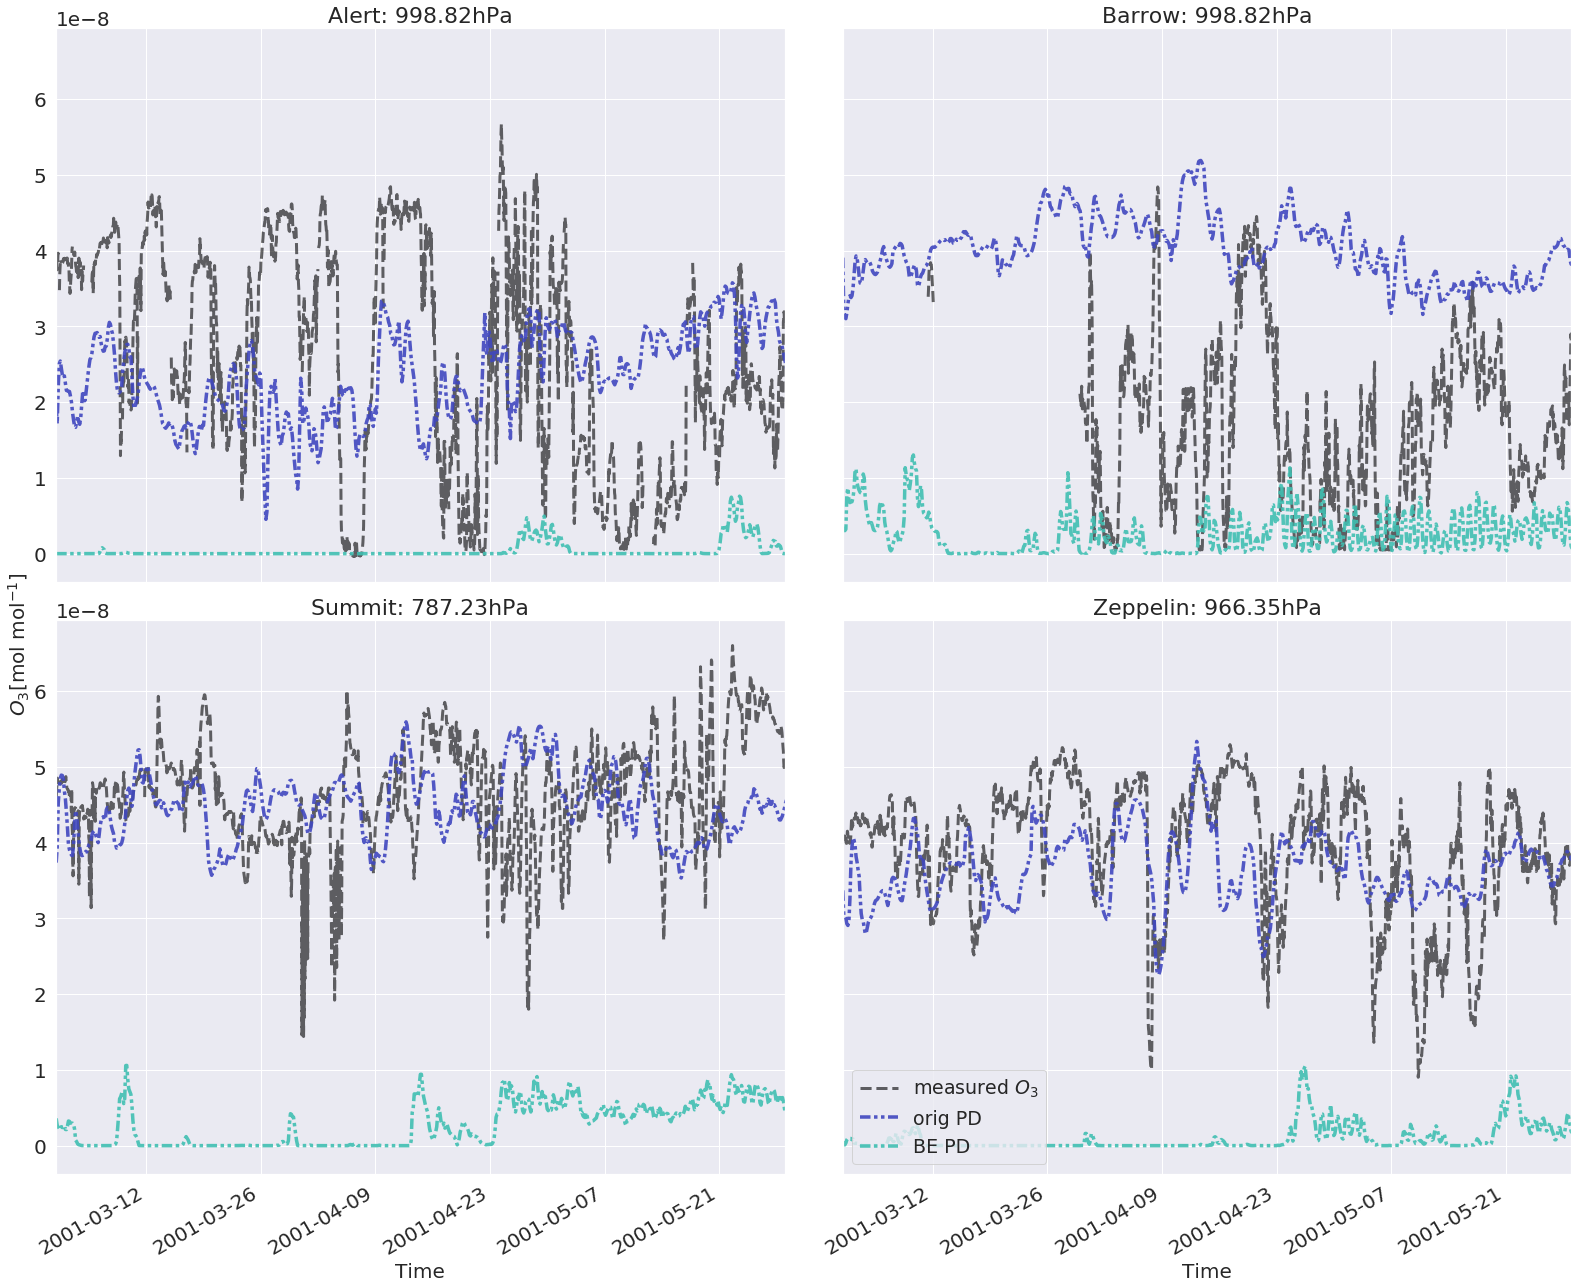
\includegraphics[width = \linewidth]{Chapter6_Results/images/ozone_stationComp_2001/ozone_2001_compObsOrigBE.png}
    \caption{Ozone measurements (black line) and model results from the original CTM3 (Branch \ref{def:origCTM3_PD}) (blue line) and Branch \ref{def:BE_PD} (turquoise line) at the four different stations, Alert (top left), Barrow (top right), Summit (lower left) and Zeppelin (lower right) with available measurements in 2001. Model results were taken from the approximate altitude of the station in hPa\protect\footnotemark}
    \label{fig:CompObsOrigBE}
\end{figure}

\footnotetext{PD = present day, BE = bromine explosion}



\subsection{Test: Removing Heterogeneous Reactions}

Figure \ref{fig:test_RemoveHetReacts} shows results in terms of $\chem{O_3}$-concentration from attempting to turn off different heterogeneous reactions, namely snow/ice reactions (described in Section \ref{sec:snow_ice_react}), heterogeneous reactions over aerosol surfaces (described in Section \ref{sec:aerosol_react}) as well as heterogeneous reactions involving chlorine and bromine, respectively. The runs were initiated with the same restart file (spin-up) as Branch \ref{def:BE_PD}. For this purpose, four new branches were created (for a full overview of the branches, see Table \ref{tab:branches}). These were:

\begin{mydef}\label{def:BE_PD_noAerosol}
    \texttt{marikoll\_bromine\_explosion\_noHetAerosol}: Branch \ref{def:BE_PD} without heterogeneous aerosol reactions (Reaction \ref{R:8}). 
\end{mydef}

\begin{mydef}\label{def:BE_PD_noIce}
    \texttt{marikoll\_bromine\_explosion\_noSnowIce}: Branch \ref{def:BE_PD} without heterogeneous reactions over ice surfaces (called \texttt{noSnowIce} by mistake) (Reaction \ref{R:7}).
\end{mydef}

\begin{mydef}\label{def:BE_PD_noCl}
    \texttt{marikoll\_bromine\_explosion\_noHetChlorine}: Branch \ref{def:BE_PD} without heterogeneous reactions involving chlorine (Reaction \ref{R:8} and \ref{R:7} with $\chem{X} = \chem{Cl}$).
\end{mydef}

\begin{mydef}\label{def:BE_PD_noBr}
    \texttt{marikoll\_bromine\_explosion\_noHetBromine}: Branch \ref{def:BE_PD} without heterogeneous reactions involving bromine (Reaction \ref{R:8} and \ref{R:7} with $\chem{X} = \chem{Br}$).
\end{mydef}


\begin{table}
\centering
\begin{tabular}{|ll|}
\hline
\textbf{Branch}                                      & \textbf{Reference}          \\ \hline
\texttt{marikoll\_originalCTM3\_NoStrat}             & \ref{def:origCTM3_PD}     \\
\texttt{marikoll\_originalCTM3\_noStrat\_pi}         & \ref{def:origCTM3_PI}     \\
\texttt{marikoll\_bromine\_explosion\_susanne}       & \ref{def:BE_PD}           \\
\texttt{marikoll\_bromine\_explosion\_PI}            & \ref{def:BE_PI}           \\
\texttt{marikoll\_bromine\_explosion\_noHetAerosol}  & \ref{def:BE_PD_noAerosol} \\
\texttt{marikoll\_bromine\_explosion\_noSnowIce}     & \ref{def:BE_PD_noIce}     \\
\texttt{marikoll\_bromine\_explosion\_noHetChlorine} & \ref{def:BE_PD_noCl}      \\
\texttt{marikoll\_bromine\_explosion\_noHetBromine}  & \ref{def:BE_PD_noBr}      \\ \hline
\end{tabular}
\caption{Overwiew of brances used in the developing process. References refer to chapter and branch number}
\label{tab:branches}
\end{table}


\begin{figure}
    \centering
    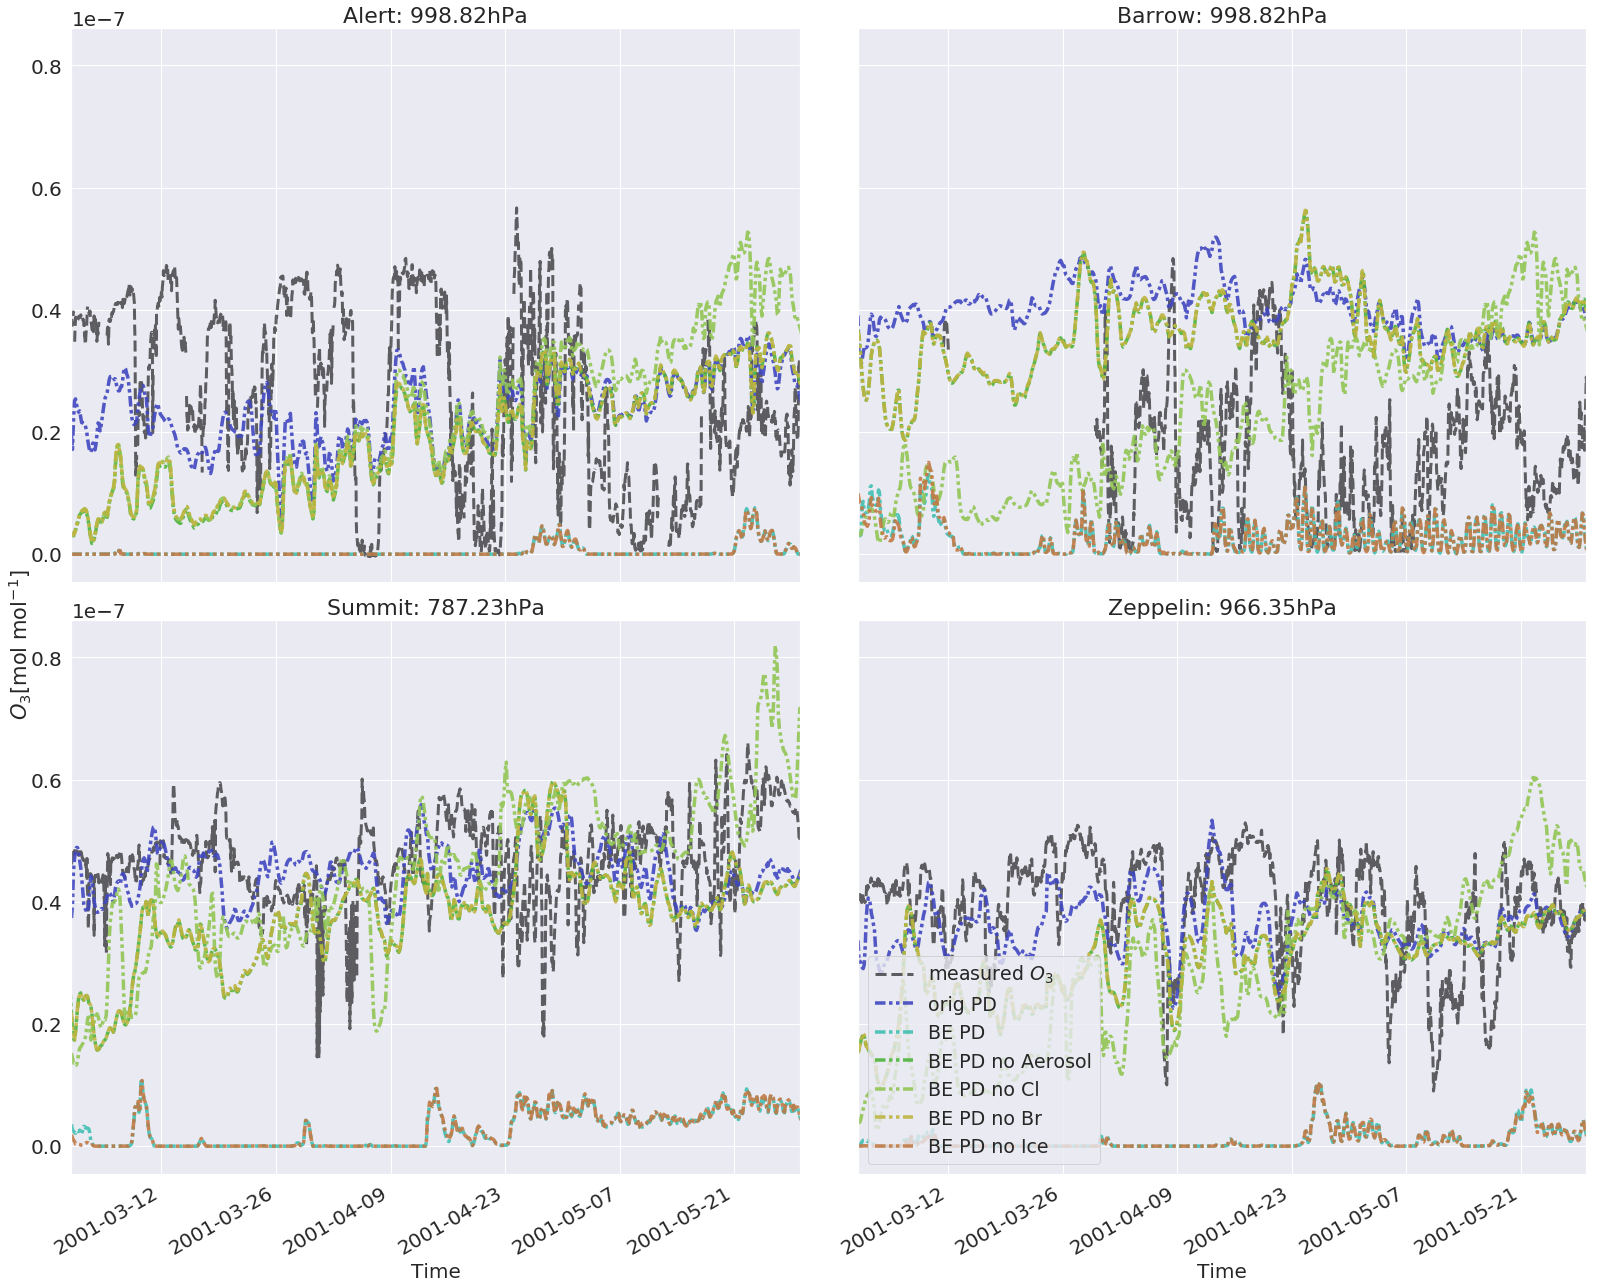
\includegraphics[width = \linewidth]{Chapter6_Results/images/ozone_stationComp_2001/ozone_2001_testRemoveHetReacts.png}
    \caption{Ozone measurements (black line) and model results from the original CTM3 (blue line), Branch \ref{def:BE_PD} (turquoise line), Branch \ref{def:BE_PD_noAerosol} (green line), \ref{def:BE_PD_noIce} (orange line), Branch \ref{def:BE_PD_noCl} (light green line) and Branch \ref{def:BE_PD_noBr} (yellow line) at the four different stations, Alert (top left), Barrow (top right), Summit (lower left) and Zeppelin (lower right) with available measurements in 2001. Model results were taken from the approximate altitude of the station in hPa. PD = present day, BE = bromine explosion}
    \label{fig:test_RemoveHetReacts}
\end{figure}


\medskip

Figure \ref{fig:vertHBr_noCl} (see Appendix \ref{app:CTM3_dev}) shows the vertical column above the Alert, Barrow, Summit and Zeppelin of the mixing ratio of \chem{HBr}. The mixing ratio is on the order $10^{-15}$ (0.001 ppt). The vertical distribution appears to be constrained with higher concentration in the lower layers at Alert, whilst increasing with altitude at Zeppelin. Seen in relation with Figure \ref{fig:polarHBr_noCl} (see Appendix \ref{app:CTM3_dev}), the concentration in the lowest layer across the Arctic is on the order of $10^{-10} - 10^{-11} g m^{-3}$

\medskip

In Figure \ref{fig:polarBrO_noCl} (see Appendix \ref{app:CTM3_dev}), the vertical column density for the lowermost $\sim$ 250 m is plotted. The column density is on the order $10^{6}$ molecules cm$^{-2}$

%In the vertical, the corresponding $\chem{Br_y}$ concentrations to Figure \ref{fig:test_RemoveHetReacts} are shown in Figures \ref{fig:vert_noAer_bry_2001}-\ref{fig:vert_noBr_bry_2001} for the four new branches, Branch \ref{def:BE_PD_noAerosol}-\ref{def:BE_PD_noBr}, respectively (The $\chem{Br_y}$-family is explained in Section \ref{sec:halogen_families_BryClxCly}). 



%\begin{figure}
    \centering
    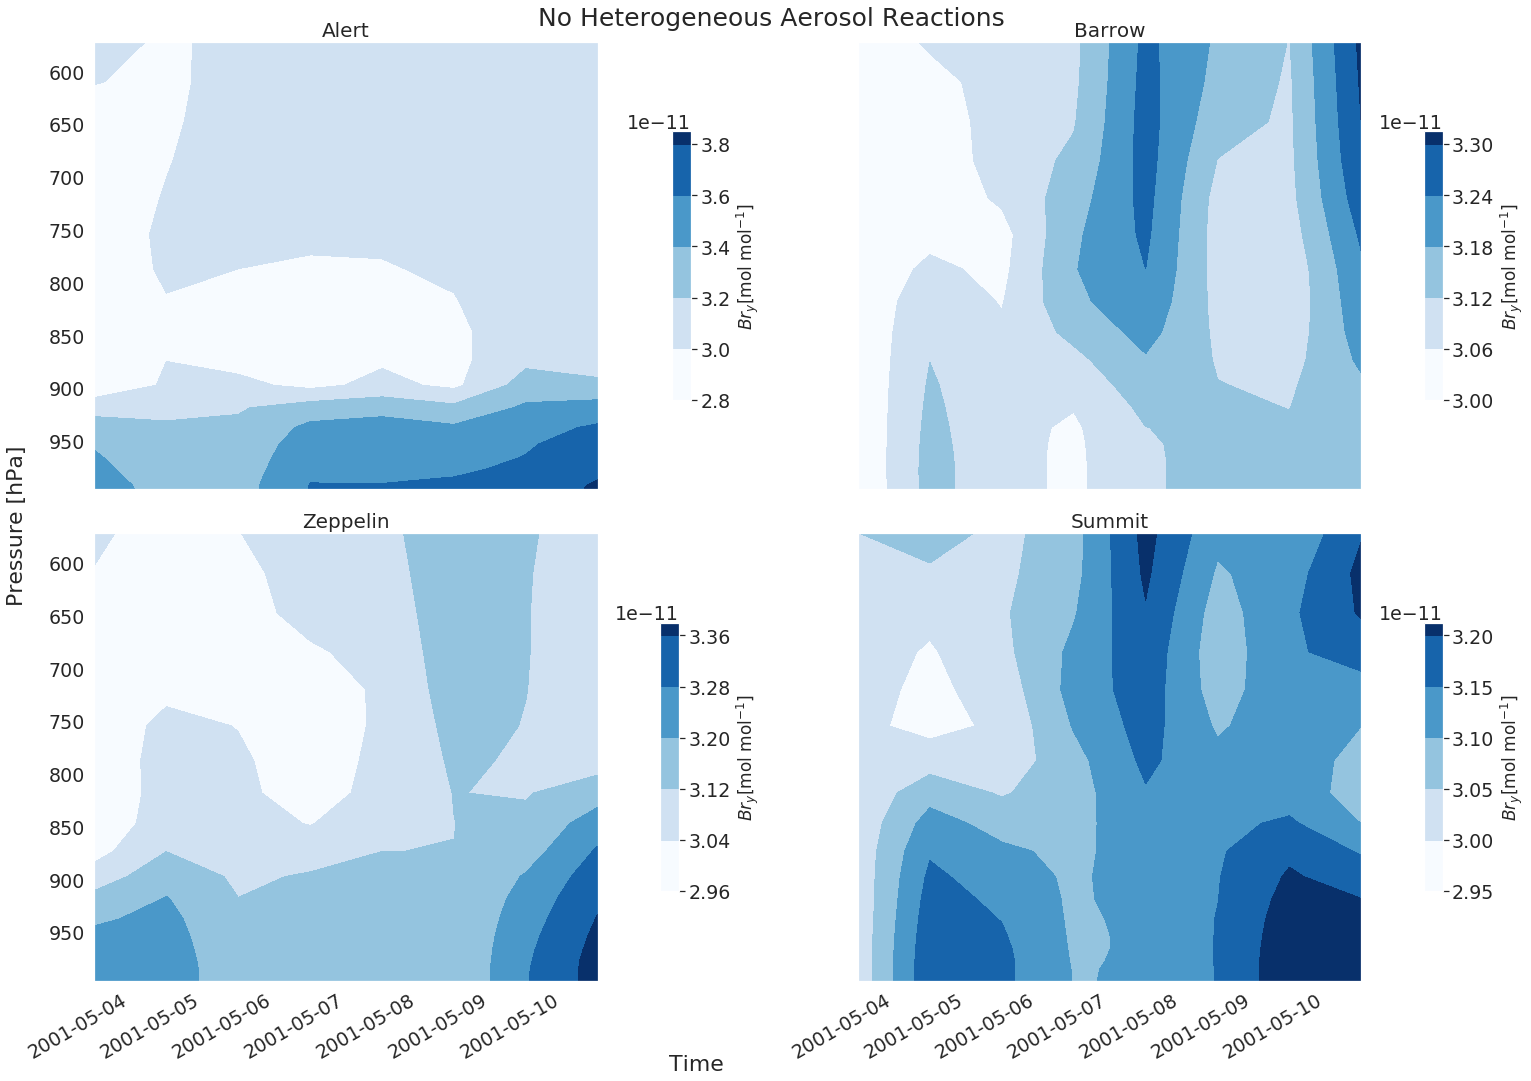
\includegraphics[width = \linewidth]{Chapter6_Results/images/noAerosol_2001_bry.png}
    \caption{Modelled $\chem{Br_y}$ without the heterogeneous aerosol reactions. The y-axis shows altitude up to 600 hPa at each station with ozone measurements at 12:00 (UTC) (Alert, Barrow, Zeppelin and Summit) in 2001.}
    \label{fig:vert_noAer_bry_2001}
\end{figure}

%\begin{figure}
    \centering
    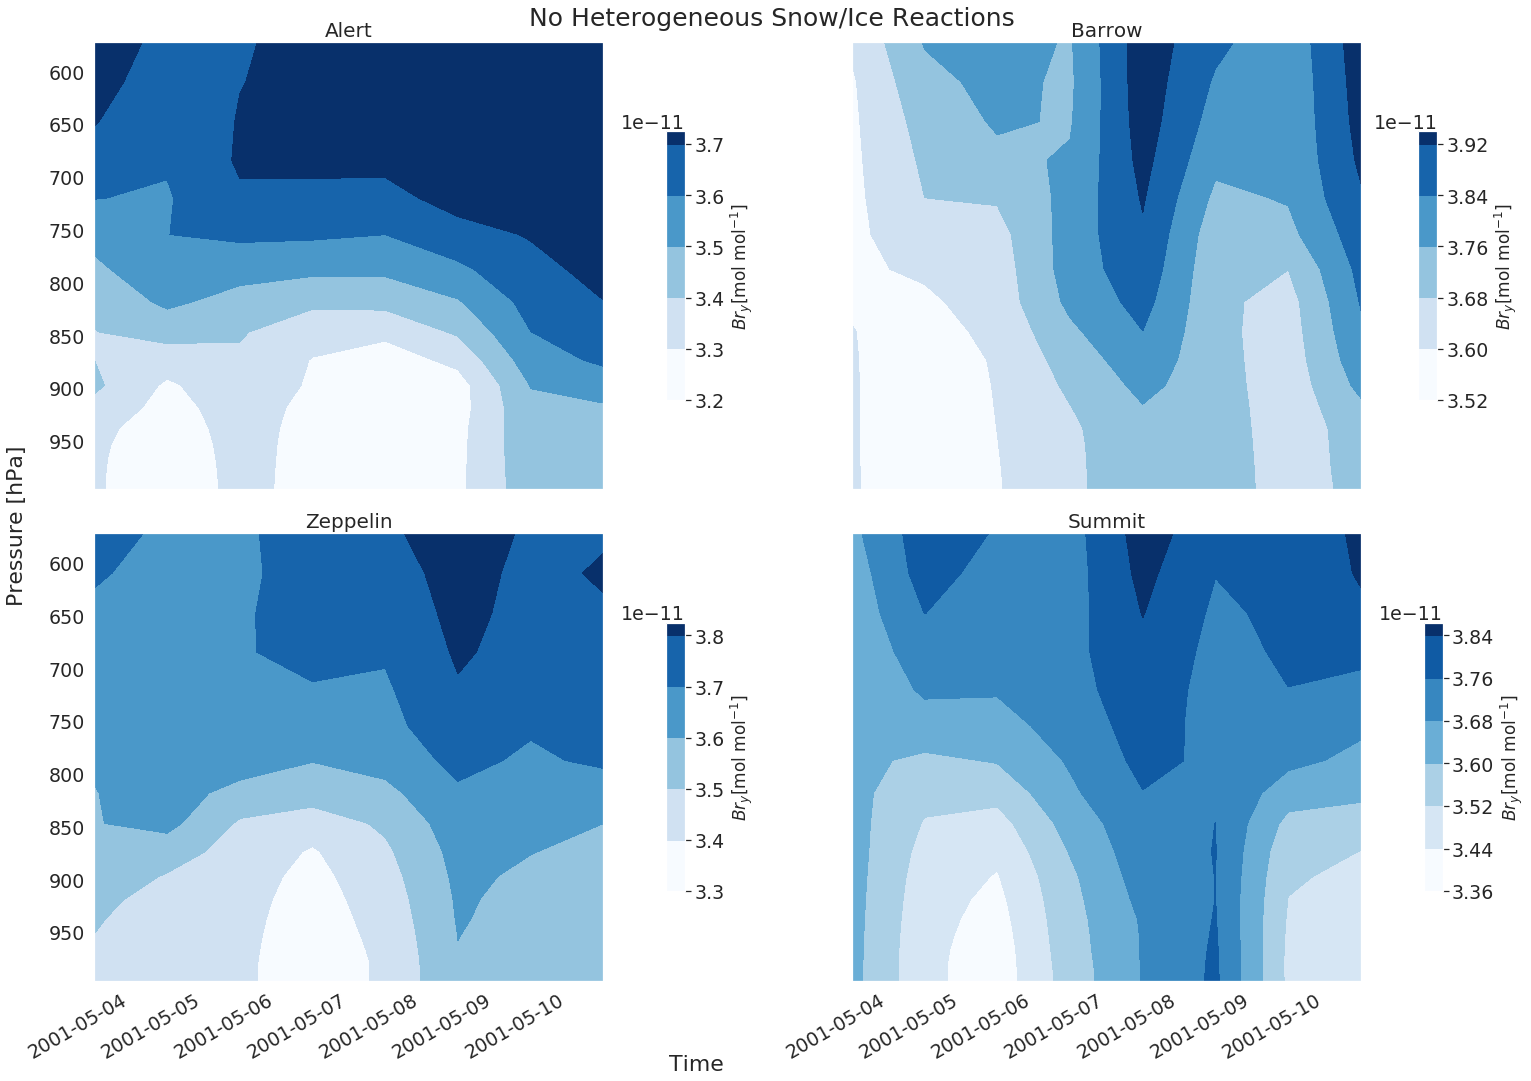
\includegraphics[width = \linewidth]{Chapter6_Results/images/noSnowIce_2001_bry.png}
    \caption{Modelled $\chem{Br_y}$ without theheterogeneous reactions over ice surfaces. The y-axis shows altitude up to 600 hPa at each station with ozone measurements (Alert, Barrow, Zeppelin and Summit) in 2001.}
    \label{fig:vert_noSnowIce_bry_2001}
\end{figure}

%\begin{figure}
    \centering
    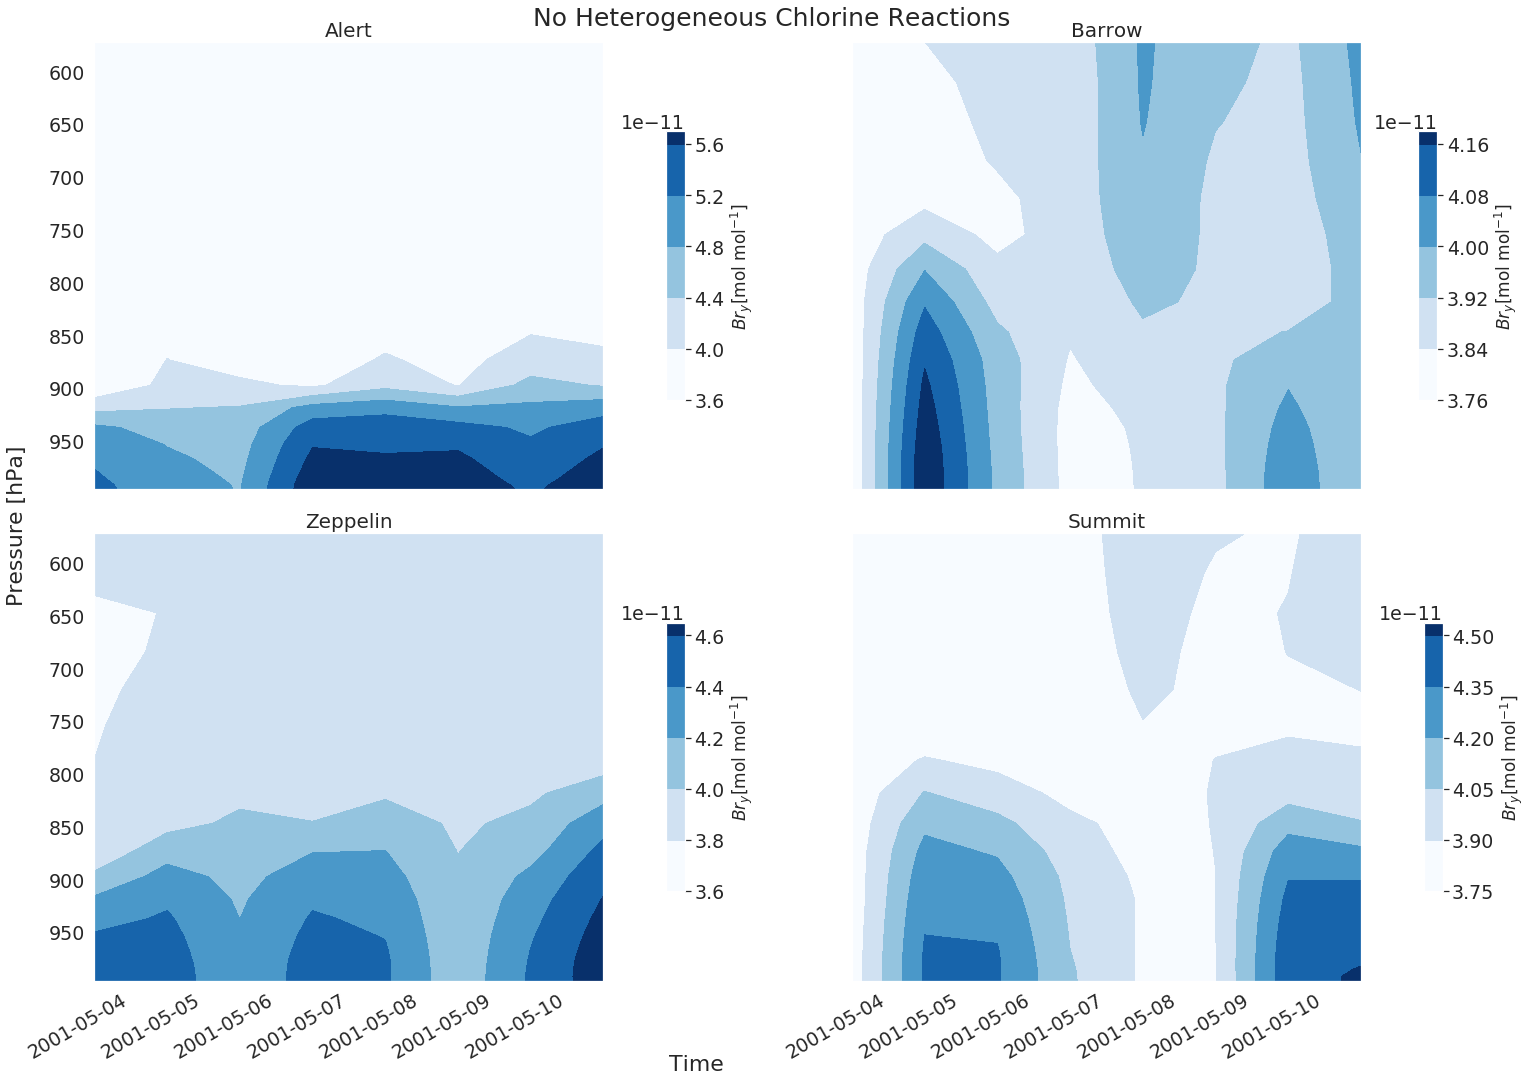
\includegraphics[width = \linewidth]{Chapter6_Results/images/noCl_2001_bry.png}
    \caption{Modelled $\chem{Br_y}$ without the heterogeneous reactions involving chlorine. The y-axis shows altitude up to 600 hPa at each station with ozone measurements (Alert, Barrow, Zeppelin and Summit) in 2001.}
    \label{fig:vert_noCl_bry_2001}
\end{figure}

%\begin{figure}
    \centering
    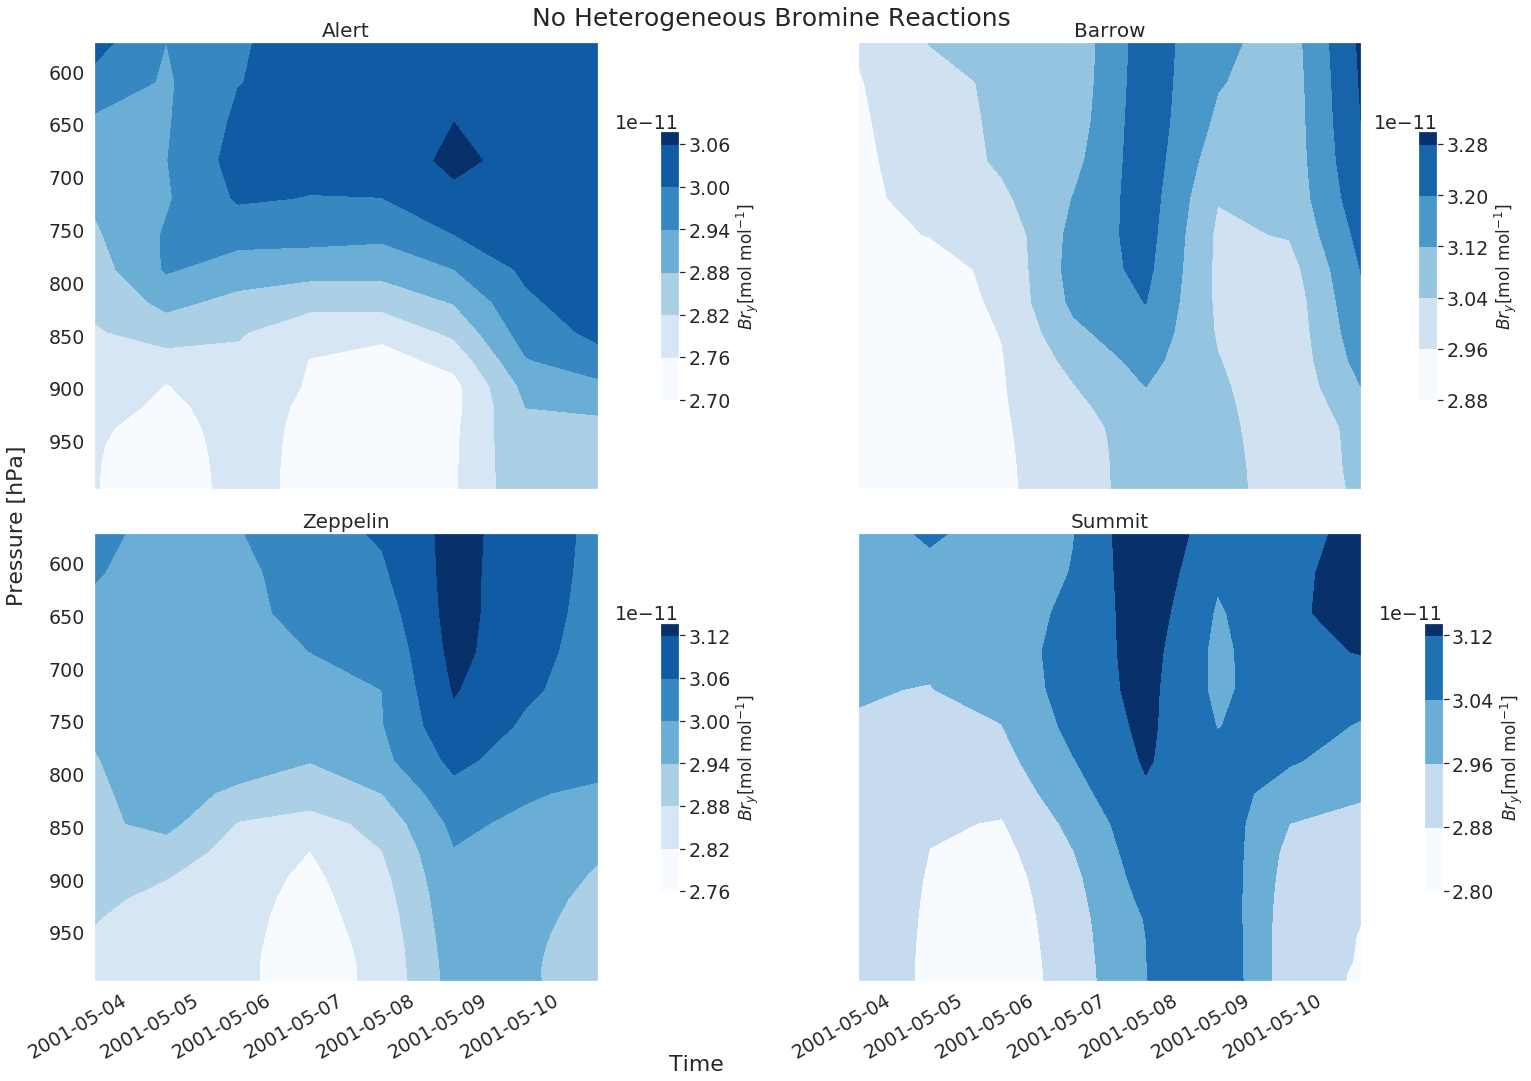
\includegraphics[width = \linewidth]{Chapter6_Results/images/noBr_2001_bry.png}
    \caption{Modelled $\chem{Br_y}$ without the heterogeneous reactions involving bromine. The y-axis shows altitude up to 600 hPa at each station with ozone measurements at 12:00 (UTC) (Alert, Barrow, Zeppelin and Summit) in 2001.}
    \label{fig:vert_noBr_bry_2001}
\end{figure}




%\textbf{NOTE:} after these tests, a mistake in the scaling of $\chem{Cl_x}$ was discovered. \chem{BrCl} had mistakenly been scaled with this family, which led to disappearance of all \chem{Cl}-species. The subsequent tests were fixed for this.

%\subsection{Integrating $\chem{Cl_y}$ in Branch \ref{def:BE_PD}}

%Figure \ref{fig:test_ClyInt} contains the result in terms of $\chem{O_3}$ concentration where an integration of the $\chem{Cl_y}$-family was added to the initial BE-branch (Branch \ref{def:BE_PD}) This integration was not handled prior to the previous model runs (the chemical families are listed in Section \ref{sec:halogen_families_BryClxCly}). 

%\medskip

%As the inclusion of $\chem{ClONO2}$ (Reaction \ref{R:clono2}) function purely as a sink to the $\chem{ClO}$, this reaction was also removed altogether to see if this would help the low chlorine levels. 

%\begin{figure}
    \centering
    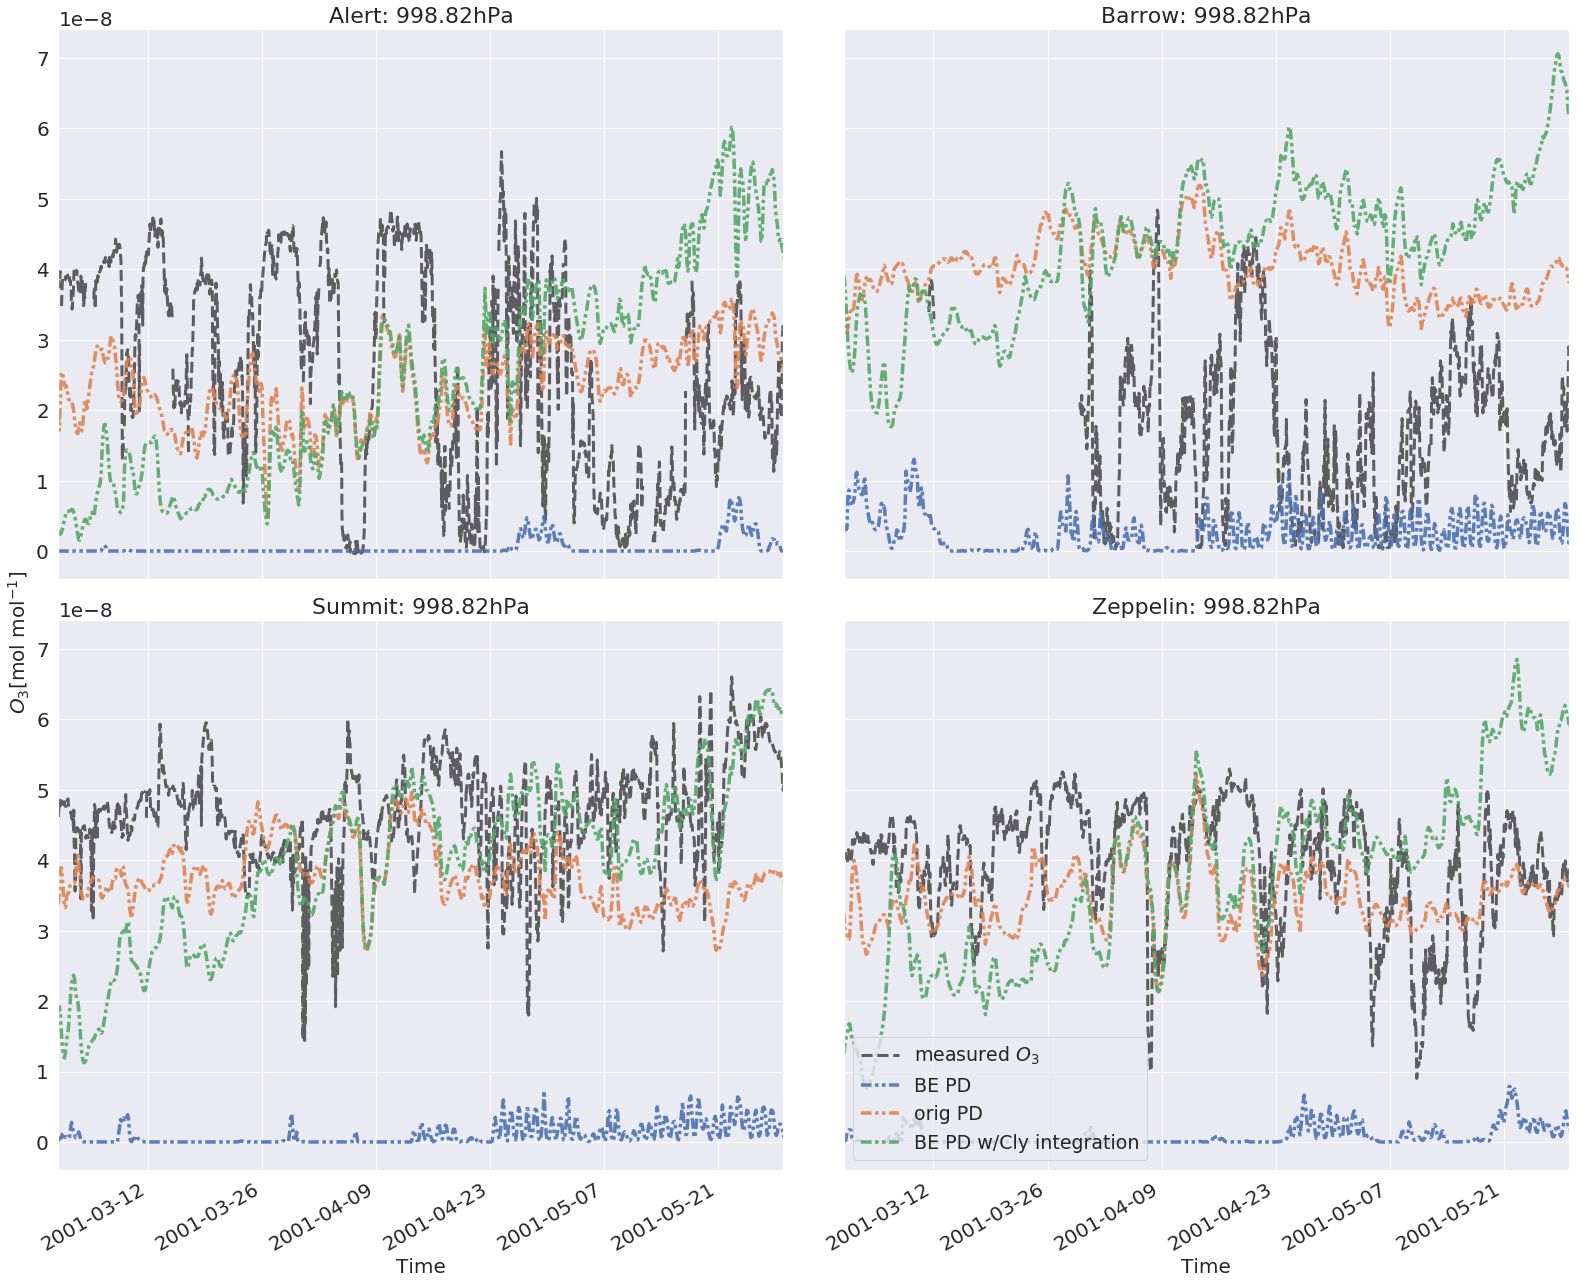
\includegraphics[width = \linewidth]{Chapter6_Results/images/ozone_2001_newClyIntegration.png}
    \caption{Ozone measurements (black line) and model results from the original CTM3 (orange line), Branch \ref{def:BE_PD} (blue line) and the attempt to integrate the $\chem{Cl_y}$ family (green line) at the four different stations, Alert (top left), Barrow (top right), Summit (lower left) and Zeppelin (lower right) with available measurements in 2001. Model results are taken from the first model level at $998.82 hPa$. PD = present day, BE = bromine explosion}
    \label{fig:test_ClyInt}
\end{figure}


\subsection{Development of Branch \ref{def:BE_PD_noCl} Without Heterogeneous Chlorine Reactions}\label{sec:res_noHetCl}

\subsubsection{Initializing Branch \ref{def:BE_PD_noCl} With a Higher \chem{HBr} Concentration}\label{sec:res_step2}

In order to boost the concentration of \chem{HBr}, the concentration was hard-coded to 30 ppt ($= 8.059\cdot10^8 \text{molecules}cm^{-3}$ at $273.15 K$) and 10 ppt ($= 2.69\cdot10^8 \text{molecules}cm^{-3}$ at $273.15 K$), respectively, in the first sub-timestep of \texttt{pchemc\_ij.f90}. Further, a run initialized with a restart file from the 10 ppt run was performed in which the hard-coded concentration of \chem{HBr} was removed.

\medskip

Figure \ref{fig:ozone_noCl_step2} contains results from different attempts to boost the \chem{HBr}-concentration, to see the effect on ozone depletion. The first test, in which the concentration of \chem{HBr} was constantly boosted by hard-coding to maintain 30 ppt (green line), results in mixing ratios of $\chem{O_3}$ comparable to the original CTM3-branch (blue line). In the second test, the \chem{HBr}-concentration was hard-coded to 10 ppt (light green line), which results in concentrations more comparable to the measurements. Lastly, the test in which the run was initiated with a restart file from the previous hard-coded test (\chem{HBr} concentration of 10 ppt) (yellow line) also maintains concentrations comparable in magnitude with the observations. All these tests were ran for a short amount of time (2 weeks to a month, model time)

\begin{figure}[ht]
    \centering
    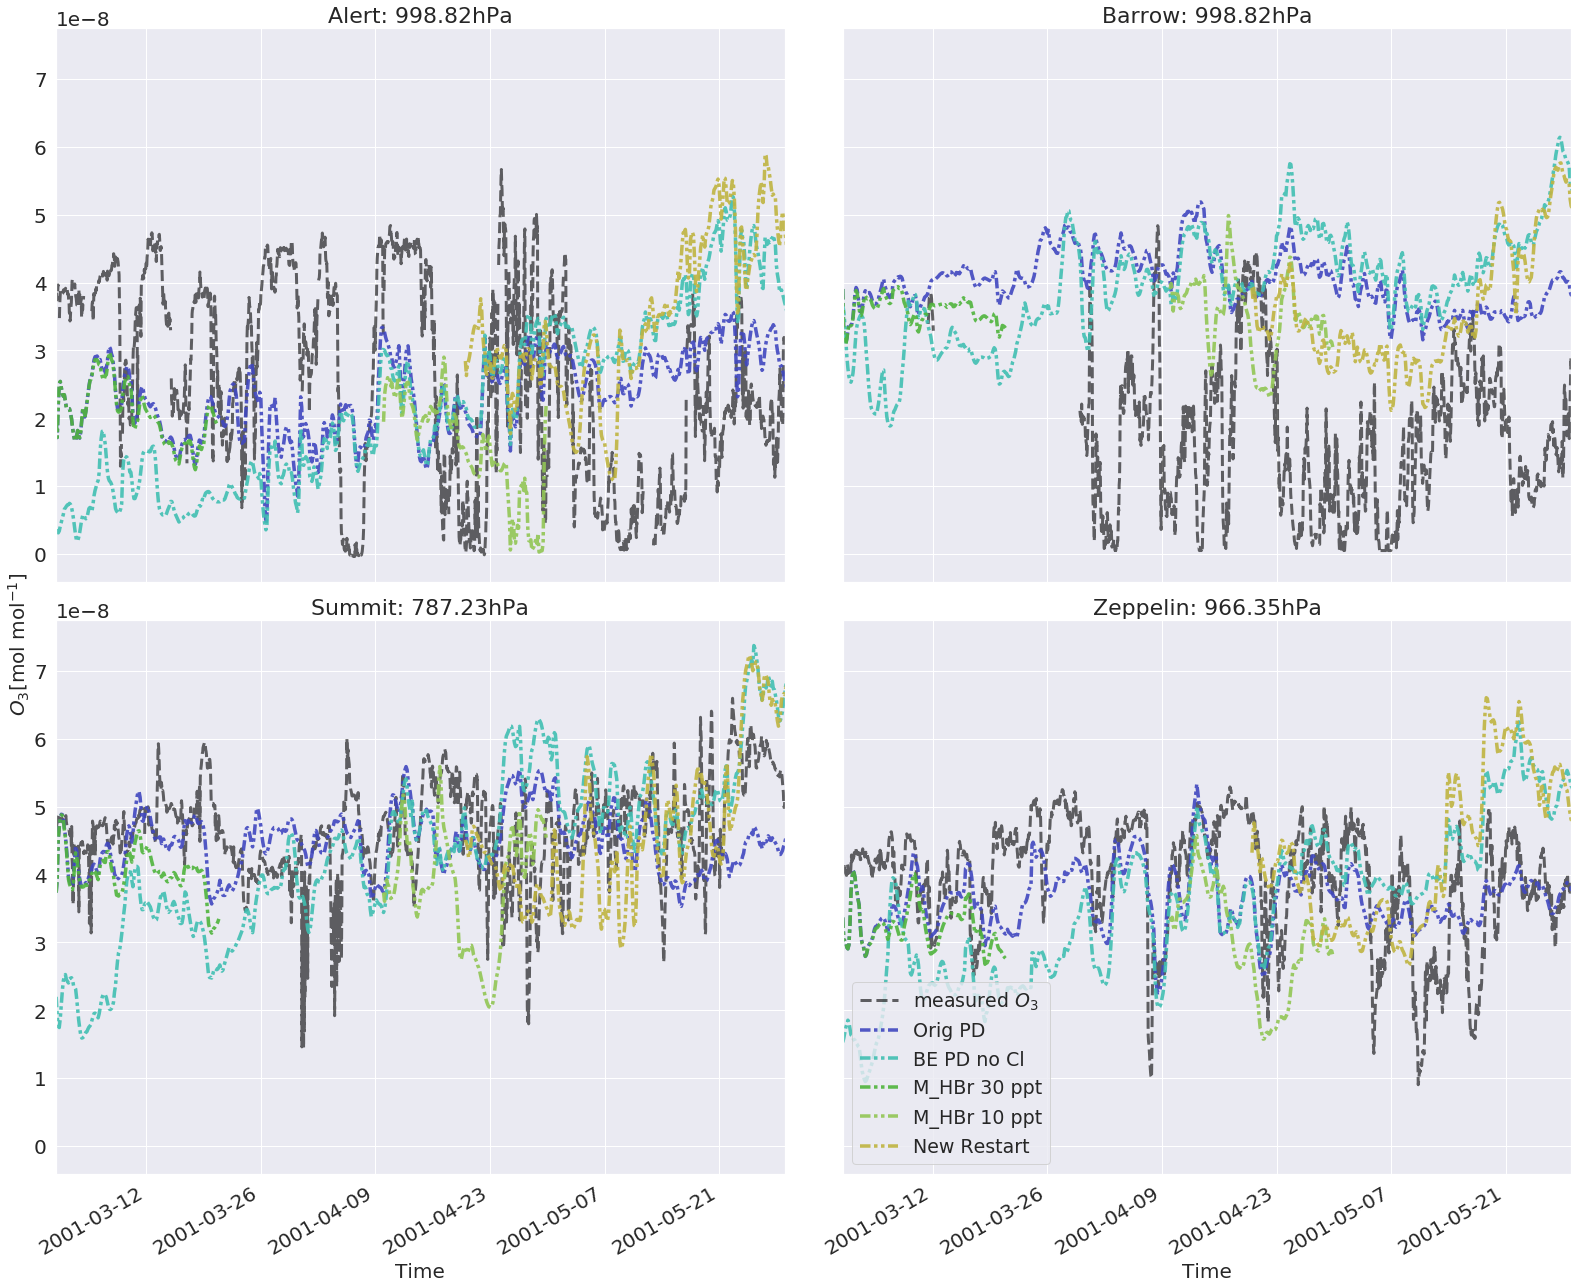
\includegraphics[width=\linewidth]{Chapter6_Results/images/ozone_stationComp_2001/ozone_noCl_step2.png}
    \caption{Ozone measurements (black line) and model results from the original CTM3 (blue line), Branch \ref{def:BE_PD_noCl} (turquoise line) (these three are the same as in Figure \ref{fig:test_RemoveHetReacts}), Branch \ref{def:BE_PD_noCl} with hard coded \chem{HBr}-concentration of 30 ppt (green line), Branch \ref{def:BE_PD_noCl} with hard coded \chem{HBr}-concentration of 10 ppt(light green line) and Branch \ref{def:BE_PD_noCl} initialized with a restart file from the hard coded \chem{HBr}-concentration of 10 ppt- run (yellow line) at the four different stations, Alert (top left), Barrow (top right), Summit (lower left) and Zeppelin (lower right) with available measurements in 2001. Model results were taken from the approximate altitude of the station in hPa}
    \label{fig:ozone_noCl_step2}
\end{figure}

\medskip

Figure \ref{fig:vertHBr_newRestart} (see Appendix \ref{app:CTM3_dev}) contains the resulting \chem{HBr}-column above Alert, Barrow, Summit and Zeppelin up to approximately $600$ hPa. The mixing ratio is on the order of $25 - 250$ ppt maximum. The higher concentrations appear to be constrained to the lower layers of the troposphere to various extents. In the lowest layer, Figure \ref{fig:polarHBr_newRestart} (see Appendix \ref{app:CTM3_dev}) shows that the concentrations are on the order of $7.5\times10^{-7} - 1.5\times10^{-6}$gm$^{-3}$. Seen in relation with Figure \ref{fig:polarHOBr_newRestart}, \ref{fig:polarHBr_newRestart} (see Appendix \ref{app:CTM3_dev}) is very anti-correlated. 



\medskip

The polar \chem{BrO}-column depicted in Figure \ref{fig:polarBro_newRestart} shows a \acrshort{vcd} on the order of $10^7 \text{molecules }$ cm$^{-2}$. 

\clearpage
\subsubsection{Hard-Coding Photodissociation and Adjusting the Henry'Law Coefficient}\label{sec:res_step3}

Figure \ref{fig:ozone_2001_step3} contains the modelled results from four new tests, whereas the original CTM3-run and the New Restart run was maintained from the previous section. Firstly, the Hard-coded P test was performed by hard-coding the photodissociation rates in \texttt{pchemc\_ij.f90}. In addition to this, two reactions were added in an attempt to better cycle the \chem{HOBr} and \chem{HBr} to avoid the anti-correlation seen in Figures \ref{fig:polarHBr_newRestart}-\ref{fig:polarHOBr_newRestart}:  

\begin{reaction}
    \chem{Br_2} + \chem{OH} \rightarrow \chem{HOBr} + \chem{Br}
    \label{rqn:oh_br2}
\end{reaction}


\begin{reaction}
    \chem{HBr} + \chem{OH} \rightarrow \chem{H_2O} + \chem{Br}
    \label{rqn:oh_hbr}
\end{reaction}

The hard-coded photodissociation rates had not previously calculated for Reactions \ref{R:18}, \ref{R:20} and \ref{R:12}. These were previously set to be solved by the fast-JX method (see Section \ref{sec:CTM3_photochemistry}), but did not work. Thus, these were hard-coded as was done previously (by \cite{Susanne}) for Reactions \ref{R:19} and \ref{R:1}. The photodissociation rates were then set to: 

\begin{itemize}
    \item $3\times10^{-4}$ s$^{-1}$ for Reaction \ref{R:18} (value from \cite{CAO})
    \item $0.014$ s$^{-1}$ for Reaction \ref{R:20}(value from \cite{CAO})
    \item $0.05\times10^{-8}$ s$^{-1}$ for Reaction \ref{R:12} (value from \cite{Papanastasiou2013}, Arctic spring dissociation rate, Figure 2, p. 3022)
\end{itemize}


%Testen viser bedring, men \chem{HBr} er fortsatt altfor høy- for treig våtavsetning? 

In the subsequent tests, the hard-coded photodissociation rates were included. These were concerning the Henry-coefficient (see Section \ref{sec:wet_dep_henrys_law}) which was initially implemented with the wrong units. The New H - low test was performed with: 


\begin{itemize}
    \item \chem{HBr}: $7.2\cdot 10^{-1} [M/amt]$, $6100 K$ (Taken from: \cite{Chameides1992})
    \item \chem{HCl}: $1.9\cdot10^1 [M/atm]$, $600 K$ (Taken from: \cite{dean1999})
\end{itemize}

The New H- high test was performed with:  

\begin{itemize}
    \item \chem{HBr}: $2.5 \cdot 10^{1} [M/amt]$, $370 K$ (Taken from: \cite{dean1999})
    \item \chem{HCl}: $1.9\cdot10^1 [M/atm]$, $600 K$ (Taken from: \cite{dean1999})
\end{itemize}

Finally, the latter was tested with a higher resolution (HTWO). 

\medskip

Figure \ref{fig:ozone_2001_step3} shows that the new tests ozone produce a lower mixing ratio than both the original CTM3 and the New Restart-test from the previous section. They also produce lower ozone concentrations at the stations compared to measurements. 

%Fin ODE klokka 21 den 29/3! Høye Br og BrO og lav ozon! (fil 88) 


\begin{figure}[ht]
    \centering
    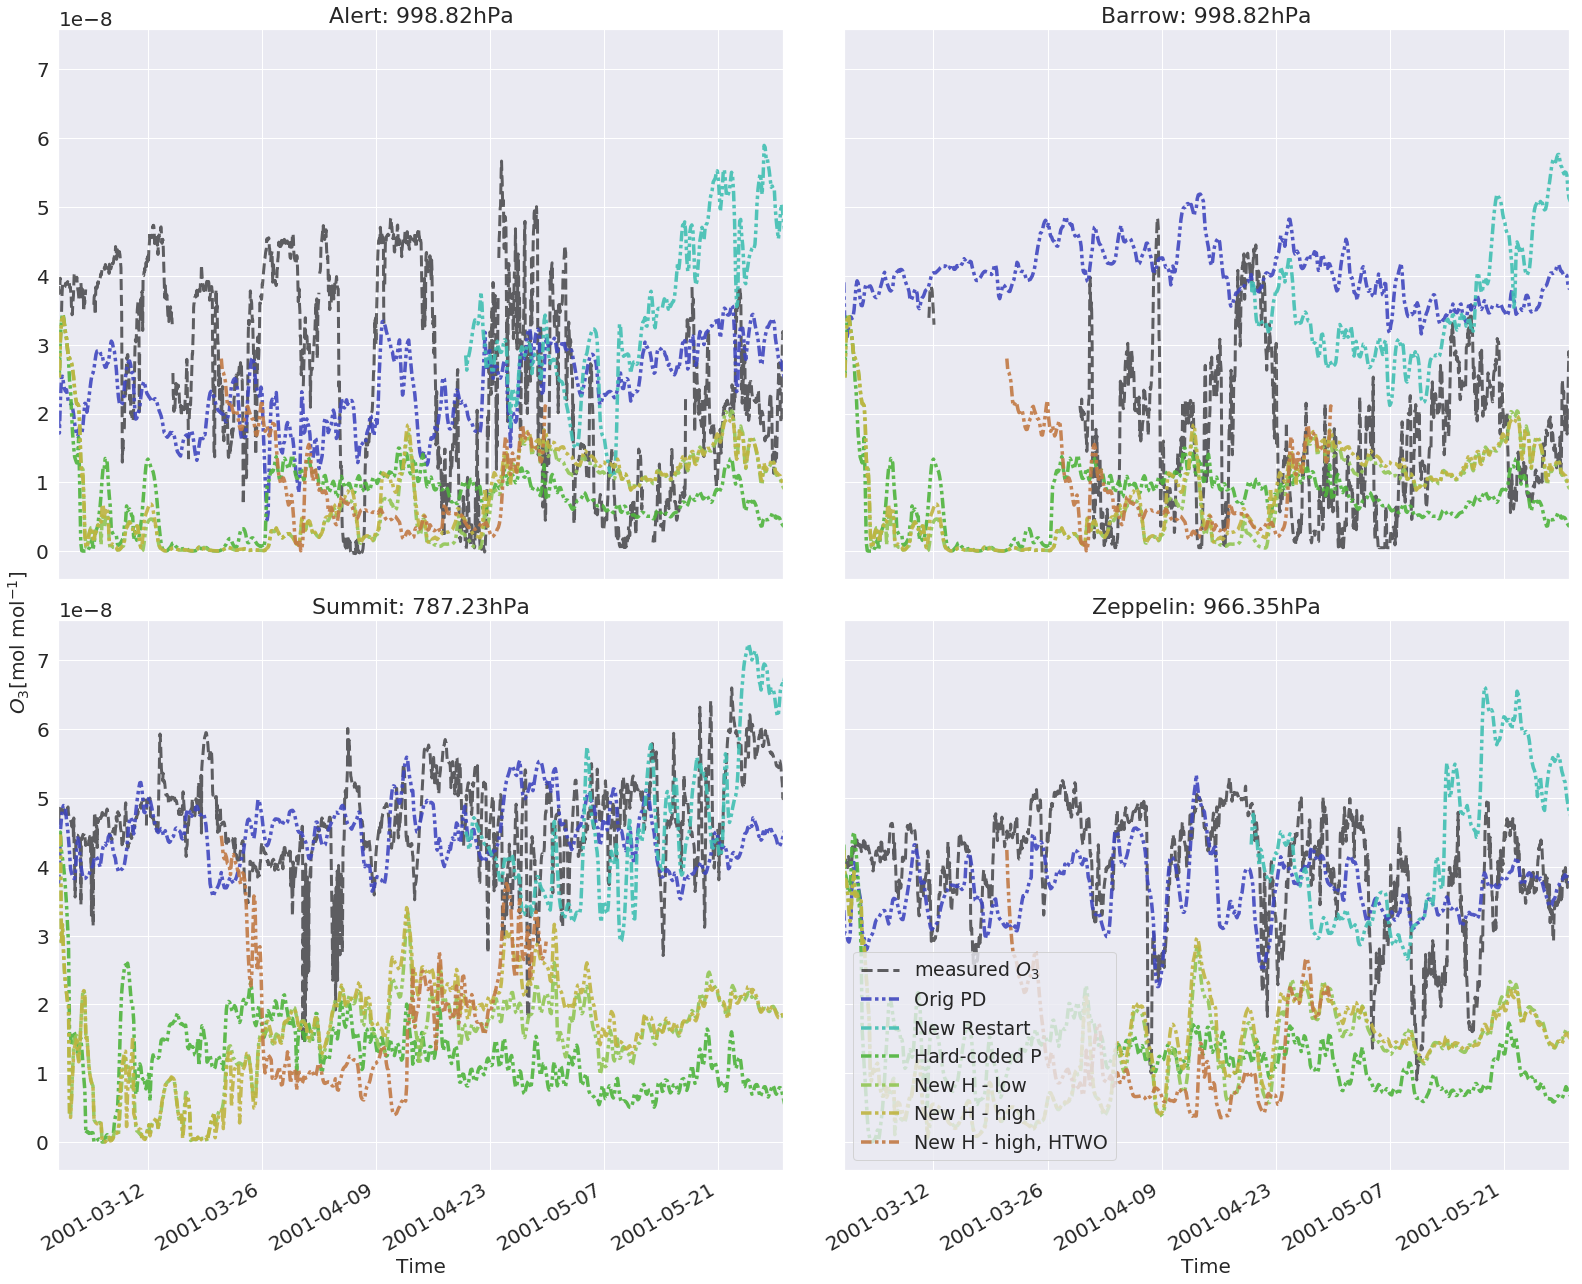
\includegraphics[width=\linewidth]{Chapter6_Results/images/ozone_stationComp_2001/ozone_2001_step3.png}
    \caption{Ozone measurements (black line) and model results from the original CTM3 (blue line) (these two are the same as in Figure \ref{fig:CompObsOrigBE}), test with new restart file from Section \ref{sec:res_step2} (turquoise line), hard-coded photodissociation rates (green line), new (low) Henry's law constant ($7.2\times10^{-1} M atm ^{-1}$, $6100 K$) (light green line), new (high) Henry's law constant ($2.5\times10^{1} M atm ^{-1}$, $370 K$) (yellow line) and the latter ran at \texttt{HTWO} resolution (orange line) at the four different stations, Alert (top left), Barrow (top right), Summit (lower left) and Zeppelin (lower right) with available measurements in 2001. Model results were taken from the approximate altitude of the station in hPa \protect\footnotemark}
    \label{fig:ozone_2001_step3}
\end{figure}

\footnotetext{H = Henry's Law}



% \begin{itemize}
%     \item \chem{HBr}: $7.2\cdot 10^{-1} [M/atm]$, $6100 K$ (Taken from: \cite{Chameides1992})
%     \item \chem{HCl}: $1.9\cdot10^1 [M/atm]$, $600 K$ (Taken from: \cite{dean1999})
% \end{itemize}

% The New H- high test was performed with:  

% \begin{itemize}
%     \item \chem{HBr}: $2.5 \cdot 10^{1} [M/atm]$, $370 K$ (Taken from: \cite{dean1999})
%     \item \chem{HCl}: $1.9\cdot10^1 [M/atm]$, $600 K$ (Taken from: \cite{dean1999})
% \end{itemize}

\medskip

Figure \ref{fig:vertHBr_HTWO_step3} (see Appendix \ref{app:CTM3_dev}) contains the vertical column of the \chem{HBr} mixing ratio at \texttt{HTWO} resolution. The mixing ratio remains around $3\times10^{-10}$ mol mol$^{-1}$ (300 ppt) for both the tests. Likewise, Figure \ref{fig:polarHBr_HTWO_step3} (see Appendix \ref{app:CTM3_dev}) contains concentrations of \chem{HBr} on the order of $6\times10^{-6} $g m$^{-3}$. The concentration of \chem{HOBr} is shown in Figure \ref{fig:polarHOBr_HTWO_step3} (see Appendix \ref{app:CTM3_dev}). The same anti-correlation is shown between \chem{HBr} and \chem{HOBr} as in the previous section. 

\medskip

The \chem{BrO} \acrshort{vcd} is shown in Figure \ref{fig:polarBrO_HTWO_step3}. The  \acrshort{vcd} now has a maximum of about $3\times10^8$ molecules cm$^{-2}$. 

\subsubsection{Higher Henry's Law Coefficient and Higher Photodissociation of \chem{HOBr}}\label{sec:res_step4}

Due to issues regarding making a final production run (i.e. running the CTM3 for 6 months) (the problems and discussion concerning this are outlined in the Discussion Section \ref{sec:disc_step4}), Branch \ref{def:BE_PD_noCl} was altered yet again with a new Henry's law constant for the wet deposition of \chem{HBr} taken from \cite{Sander99}: 

\begin{itemize}
    \item $1.3\times10^9/K_\text{A} [M/atm]$, $10 000 K$ (Taken from: \cite{Brimblecombe1988TheSA})
    \item The acid dissociation constant, $K_\text{A}$, was taken as $\ln{K_\text{A}} \approx 9.8$ (\cite{Levanov})
\end{itemize}

As well as a new photodissociation rate for \chem{HOBr}:

\begin{itemize}
    \item $3\times10^{-3}$ s$^{-1}$ for Reaction \ref{R:18} (based on value from \cite{CAO}, but an order of 10 faster)
\end{itemize}

This branch was initialized with the restart file provided from \cite{StefaniePersonal} (see Section \ref{subsec:restart_files}) and ran for 6 months runs at \texttt{HTWO} resolution. 

\medskip

The resulting ozone mixing ratio at the four stations can be seen in Figure \ref{fig:ozone_2001_step4}. The black and blue line represents the measured ozone and the results from the original CTM3, respectively. The turquoise line represents the result maintained from the section above, which was ran at \texttt{HTWO}-resolution and was supposed to be the basis for the final production run. Finally, the green line represents the actual production run, in which the differences are explained above. The final version initially produces mixing ratios comparable to both the original CTM3 and the observations. Over the course of February to mid-April, however, the ozone mixing ratio produced by the final version is quite a lot lower than the observations. Towards the end of April, the content seems to stabilize more with mixing ratios comparable to measurements at Alert and Barrow, and to some extents at Zeppelin, but much lower than what's measured at Summit. 


\begin{figure}[ht]
    \centering
    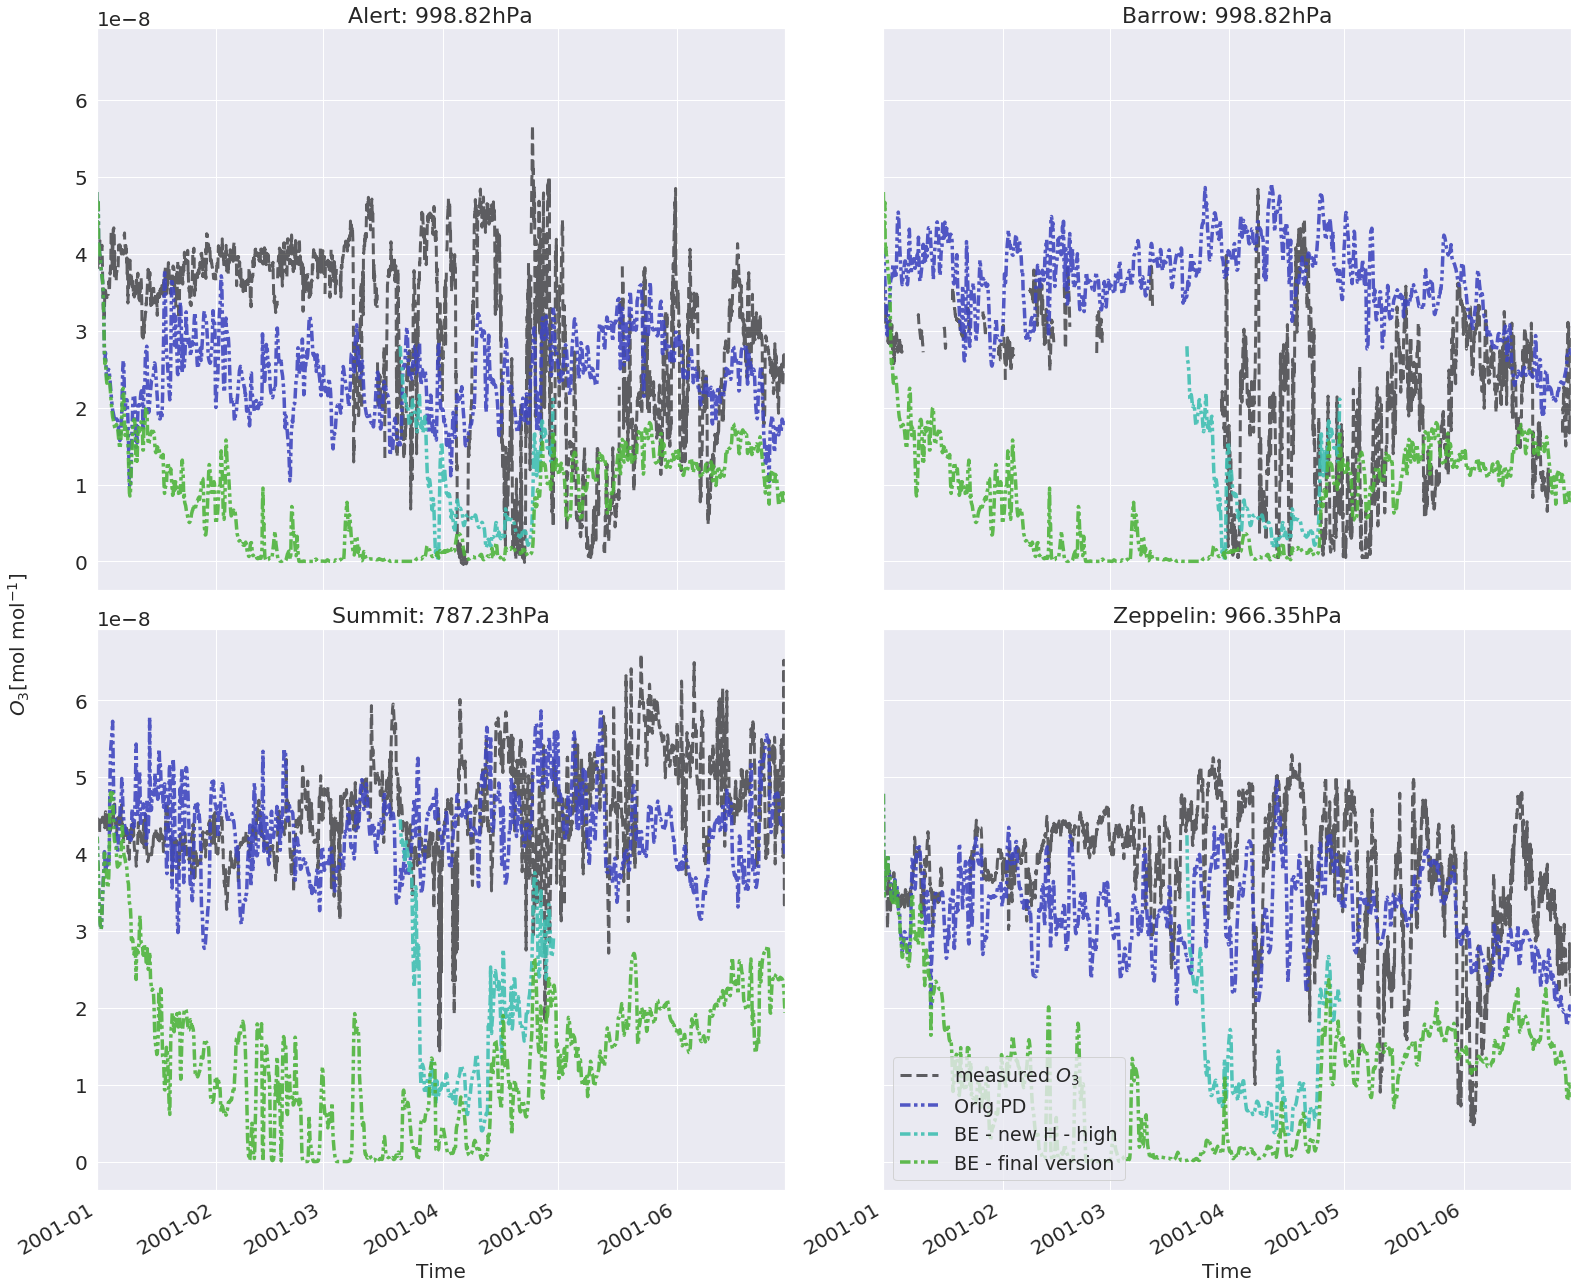
\includegraphics[width=\linewidth]{Chapter6_Results/images/ozone_stationComp_2001/ozone_2001_step4.png}
    \caption{Ozone measurements (black line) and model results from the original CTM3 (blue line) (these two are the same as in Figure \ref{fig:CompObsOrigBE}), Henry's law constant of $2.5\times10^{1} M atm ^{-1}$ and $370 K$ at \texttt{HTWO} resolution (turquoise line) and a final version with a new, higher Henry's law constant of $7.2\times10^{4} M atm ^{-1}$ and $10 000 K$ also at \texttt{HTWO} resolution (green line) at the four different stations, Alert (top left), Barrow (top right), Summit (lower left) and Zeppelin (lower right) with available measurements in 2001. Model results were taken from the approximate altitude of the station in hPa. PD = present day, P = photolysis rate, H = Henry's Law}
    \label{fig:ozone_2001_step4}
\end{figure}
\medskip

Figure \ref{fig:vertHBr_step4} contains the vertical profile of \chem{HBr} above the fours stations up to 600 hPa. The concentration is on the order of $10^{-11}$ mol/mol (10 ppt). The polar concentration in the first model layer is shown in Figure \ref{fig:polarHBr_step4}. The concentration is on the order of $10^{-7}$ gm$^{-3}$. 

\medskip


\begin{figure}[ht]
    \centering
    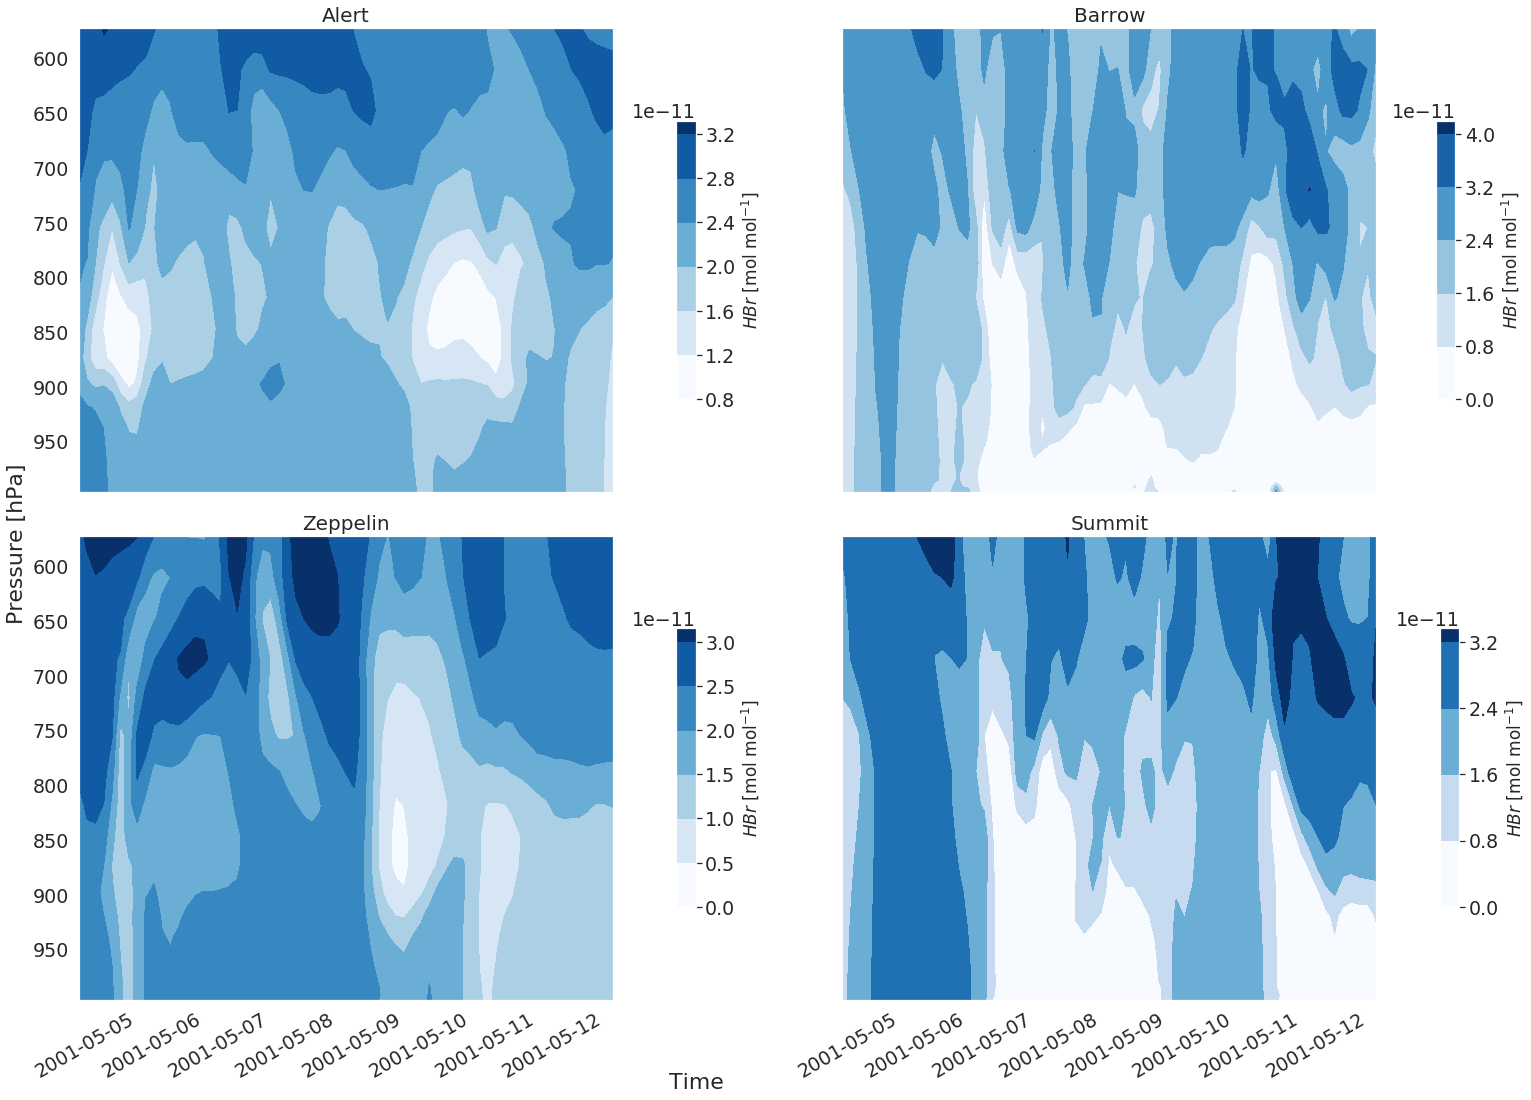
\includegraphics[width = \linewidth]{Chapter6_Results/images/Vert_StationComp_2001/vertHBr_step4.png}
    \caption{Mixing ratio ($mol mol^{-1}$) of \chem{HBr} in the model layers up to $\sim 600 hPa$ at the four different stations Alert (top left), Barrow (top right), Zeppelin (lower left) and Summit (lower right) in April-May, 2001. The results are from the final version of the CTM3}
    \label{fig:vertHBr_step4}
\end{figure}
\begin{figure}[h]
    \centering
    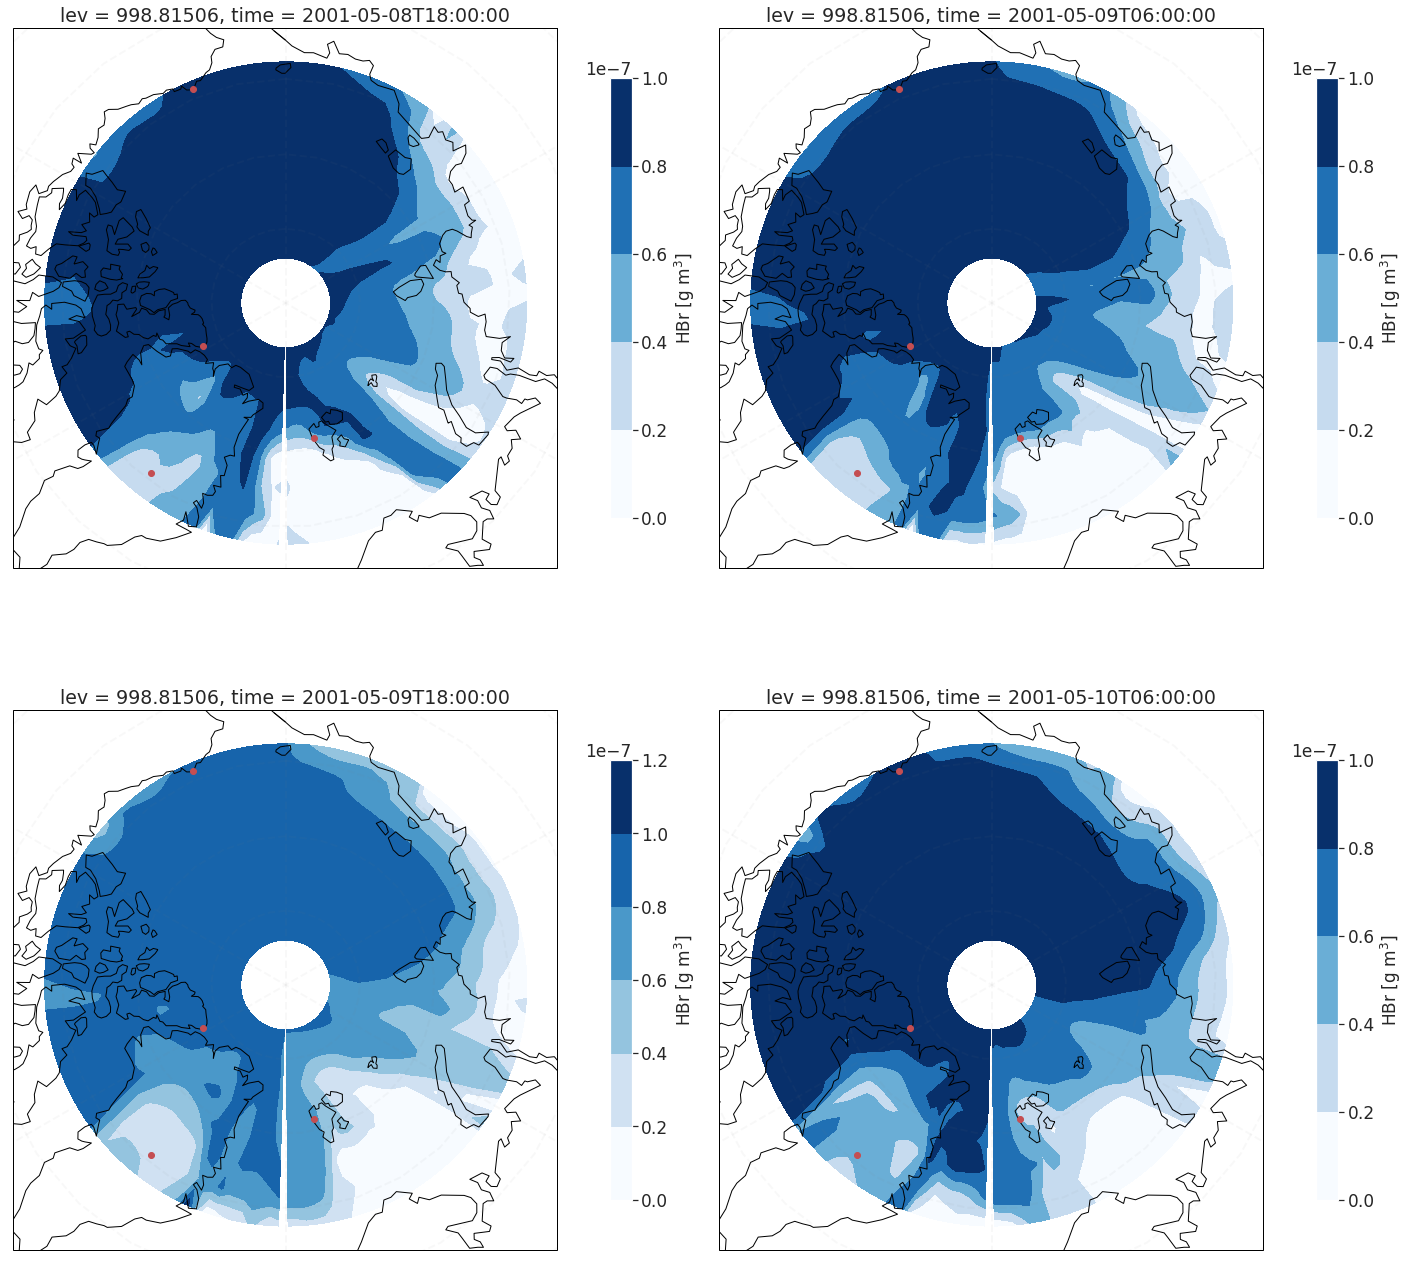
\includegraphics[width=\linewidth]{Chapter6_Results/images/Polar_StationComp_2001/HBr/polarHBr_step4.png}
    \caption{Concentration ($g m^{-3}$) of \chem{HBr} in the first model layer the Arctic at 18:00 and 06:00 (UTC) of the 22nd, 23rd and 24th of April, 2001. The result is from the test including hard-coded photodissociation rates as well as a new (high) Henry-coefficient at HFOUR resolution. The red dots are the positions of the stations with observations in 2001 (see the map in Figure \ref{fig:stns} for reference)}
    \label{fig:polarHBr_step4}
\end{figure}
\begin{figure}[h]
    \centering
    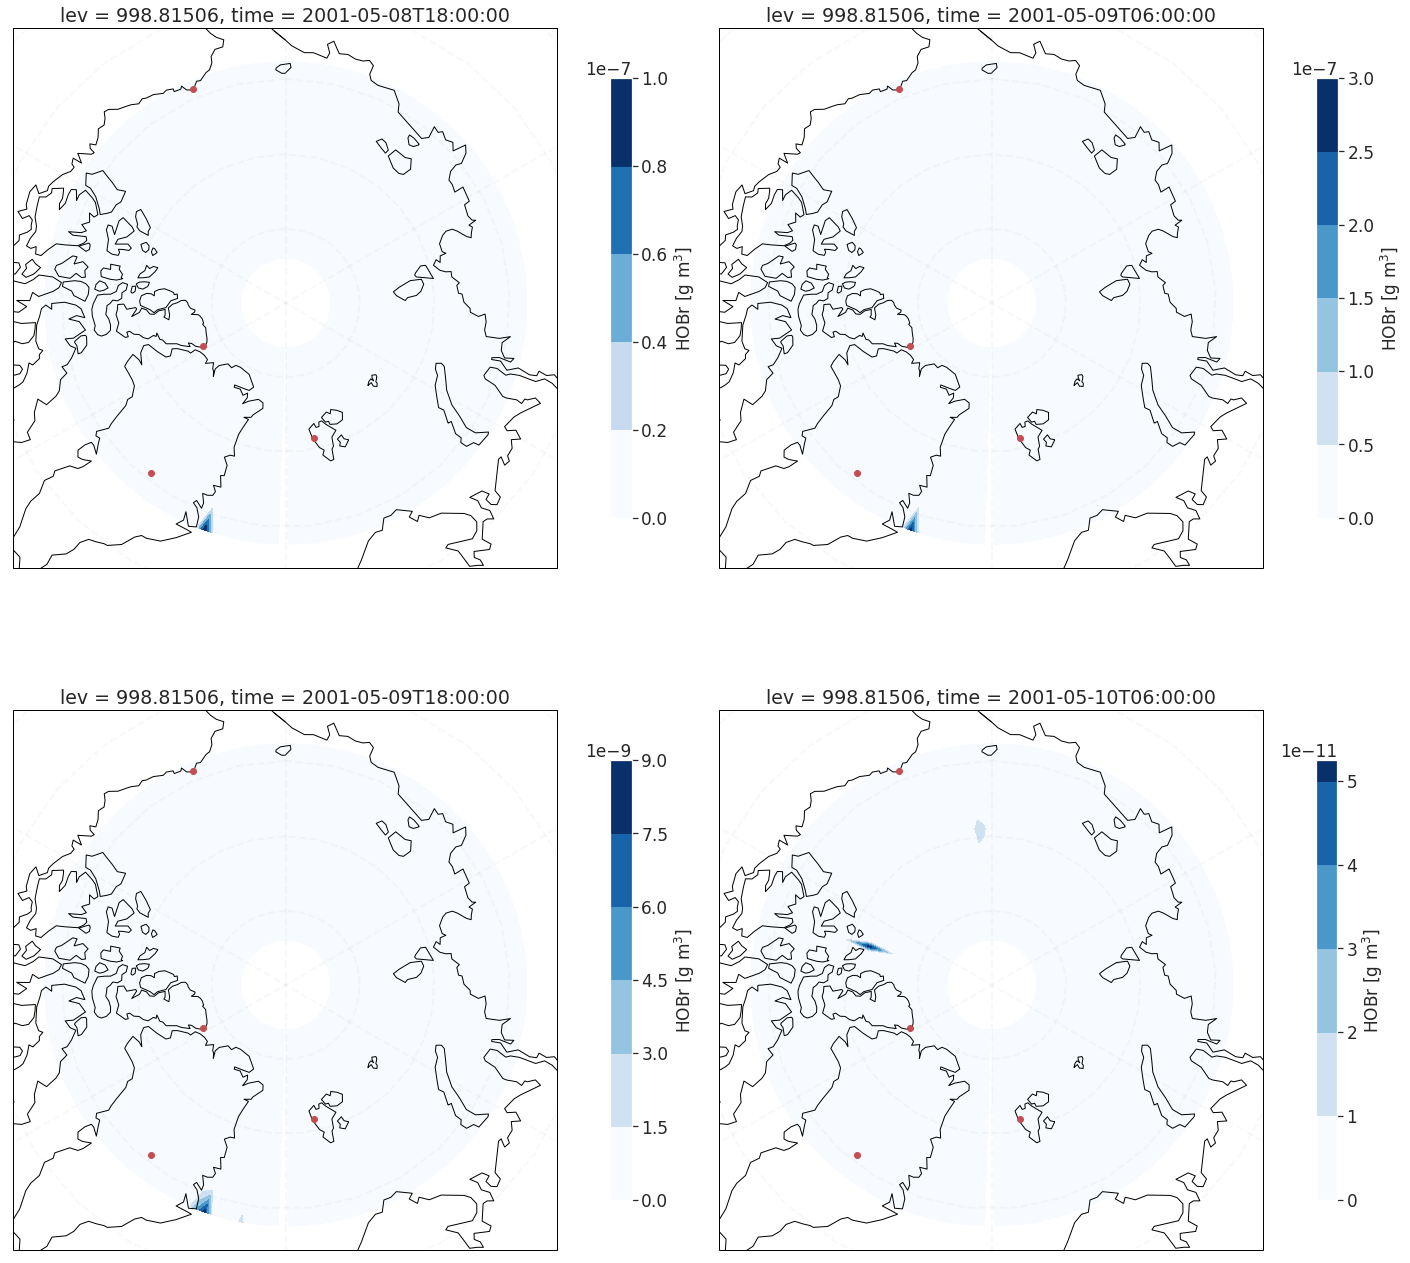
\includegraphics[width=\linewidth]{Chapter6_Results/images/Polar_StationComp_2001/HOBr/polarHOBr_step4.png}
    \caption{Concentration ($g m^{-3}$) of \chem{HOBr} in the first model layer the Arctic at 18:00 and 06:00 (UTC) of the  22nd, 23rd and 24th of April, 2001. The result is from Branch \ref{def:BE_PD_noCl} initialized with a new restart file with a \chem{HBr} concentration of 10 ppt. The red dots are the positions of the stations with observations in 2001 (see the map in Figure \ref{fig:stns} for reference)}
    \label{fig:polarHOBr_step4}
\end{figure}

\medskip

The corresponding \chem{HOBr}-concentration can be seen in Figure \ref{fig:polarHOBr_step4}. Seen in relation with Figure \ref{fig:polarHBr_step4}, the anti-correlation between the \chem{HBr} and \chem{HOBr} seems to be gone, and there is practically no \chem{HOBr} in this layer. The corresponding $\chem{O_3}$-concentration can be seen in Figure \ref{fig:polarO3_step4}.

\begin{figure}[h]
    \centering
    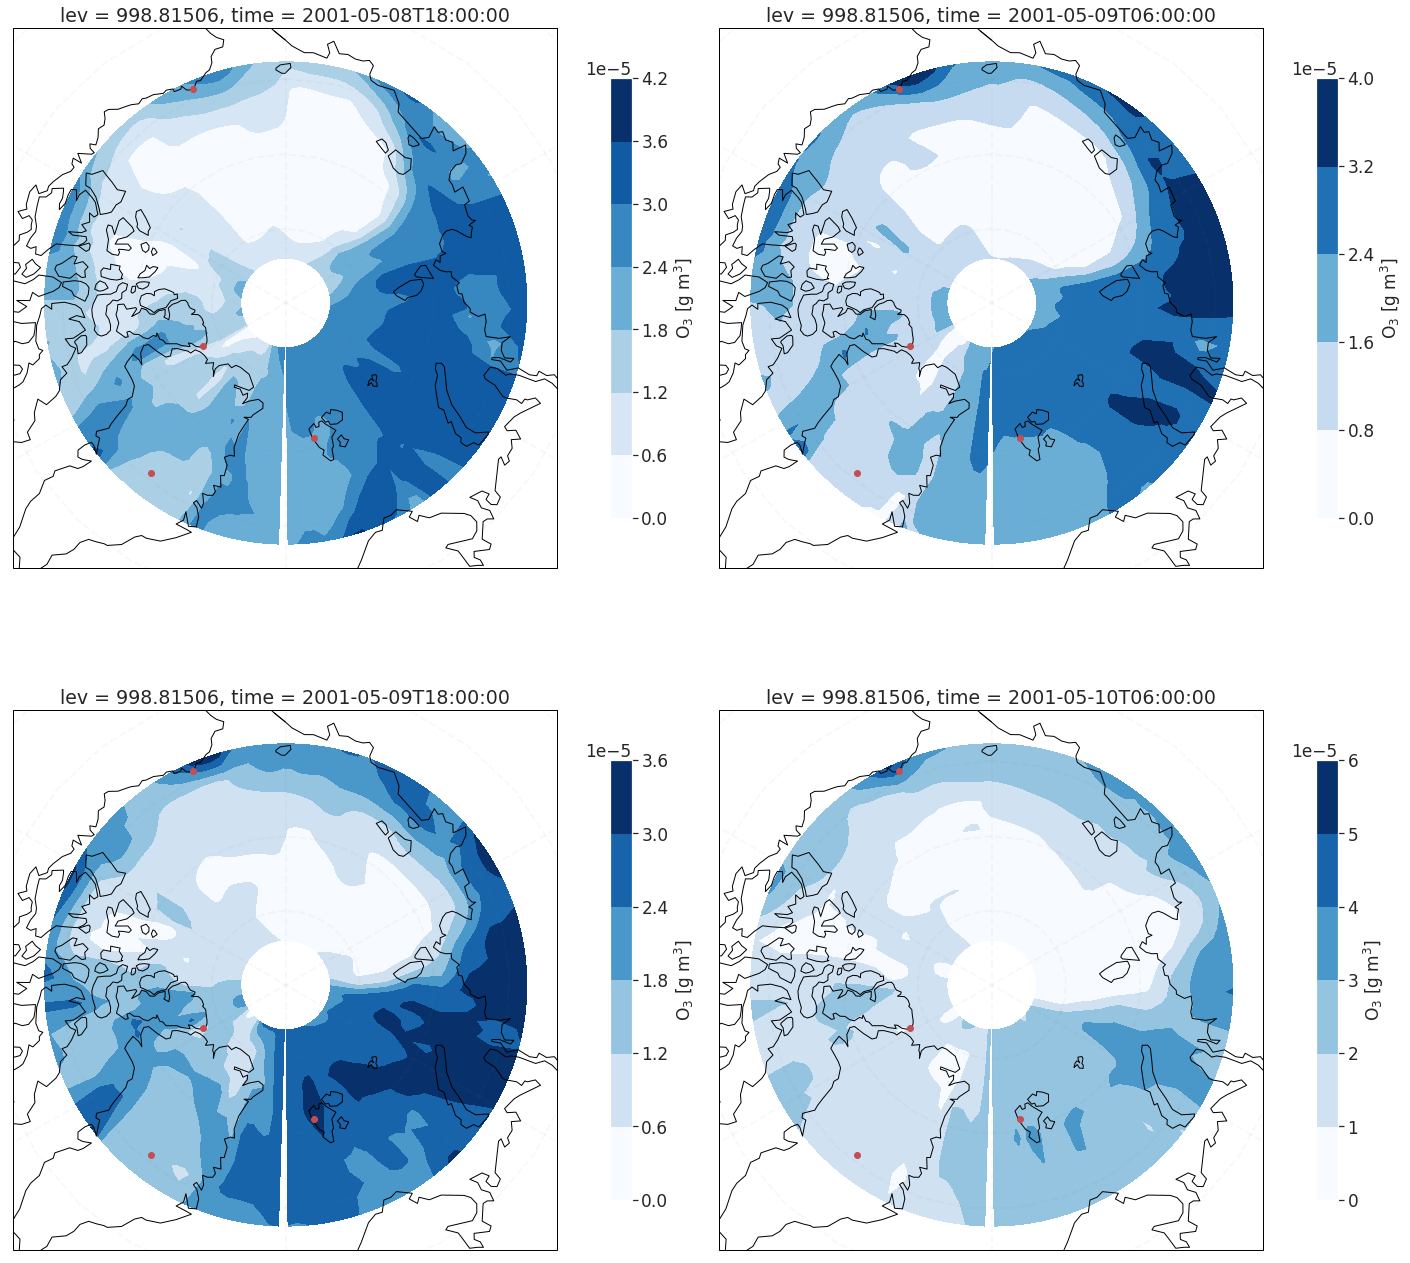
\includegraphics[width=\linewidth]{Chapter6_Results/images/Polar_StationComp_2001/O3/polarO3_step4.png}
    \caption{Concentration ($g m^{-3}$) of $\chem{O_3}$ in the first model layer the Arctic at 18:00 and 06:00 (UTC) of the  22nd, 23rd and 24th of April, 2001. The result is from Branch \ref{def:BE_PD_noCl} initialized with a new restart file with a \chem{HBr} concentration of 10 ppt. The red dots are the positions of the stations with observations in 2001 (see the map in Figure \ref{fig:stns} for reference)}
    \label{fig:polarO3_step4}
\end{figure}

\medskip

In Figure \ref{fig:polarBrO_step4}, the resulting  \chem{BrO}-\acrshort{vcd} is on the order of $10^{8}$ molecules cm$^{-2}$. 

\begin{figure}[h]
    \centering
    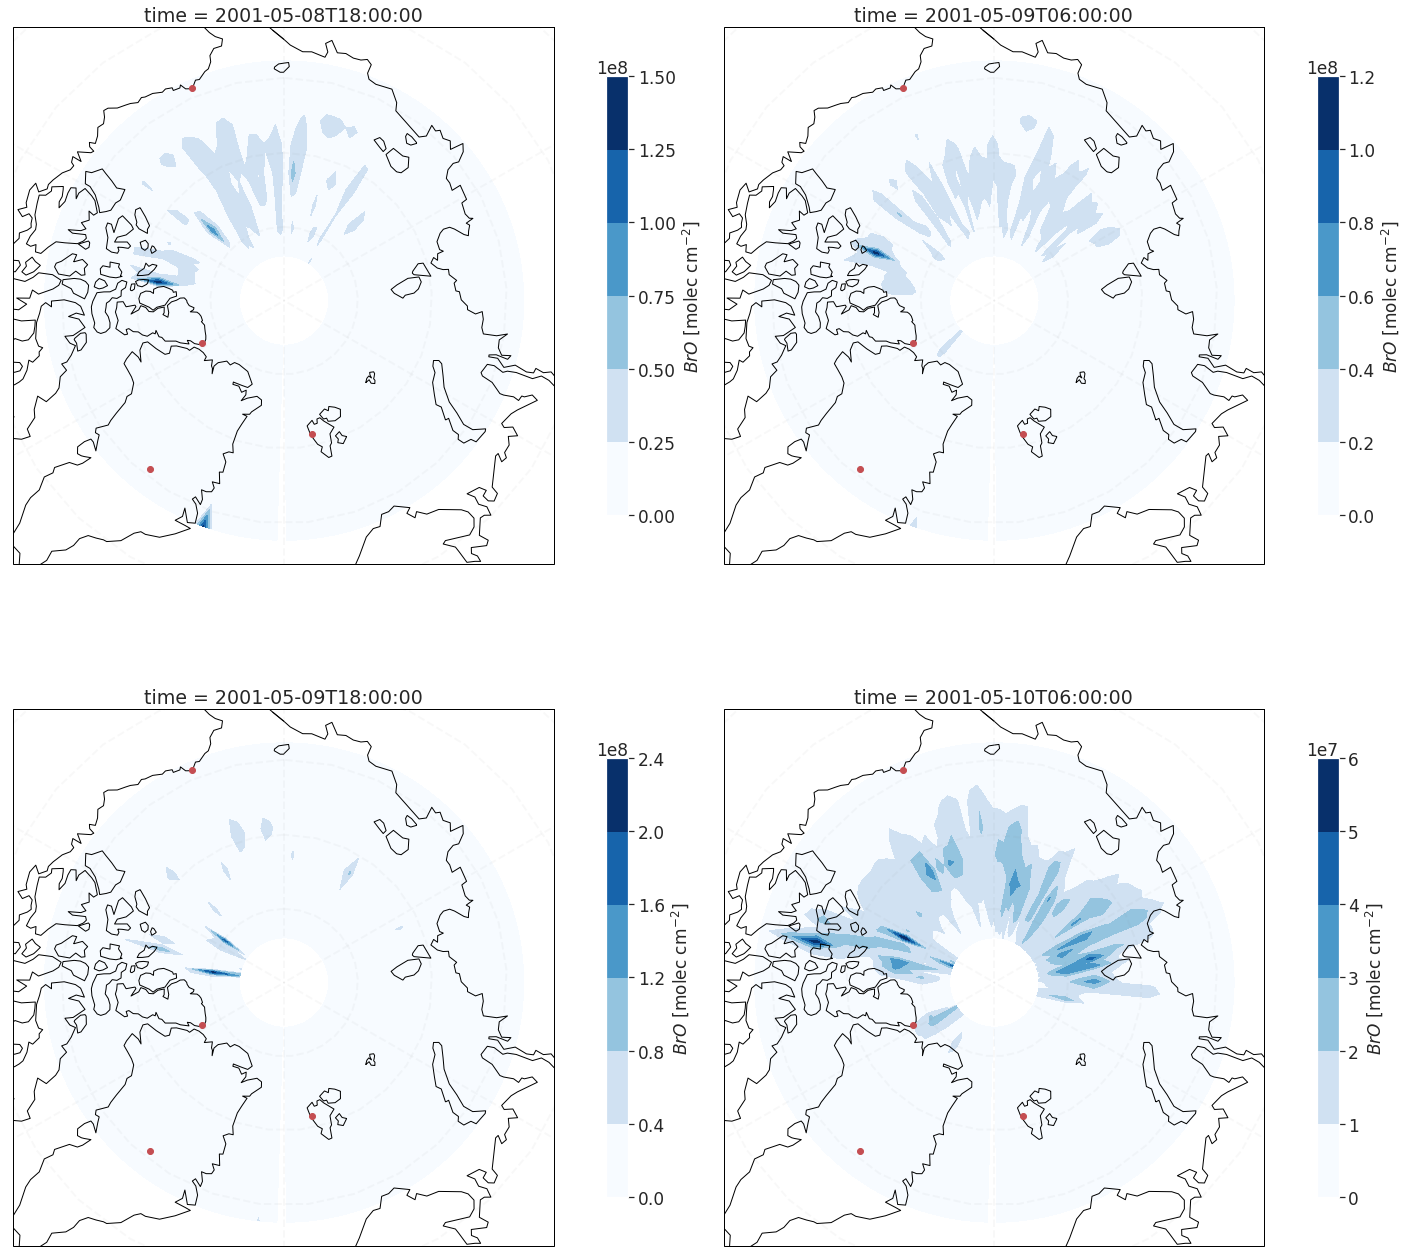
\includegraphics[width = \linewidth]{Chapter6_Results/images/Polar_StationComp_2001/BrO/polarBrO_step4.png}
    \caption{Vertical column density ($molecules cm^{-2}$) of \chem{BrO} in the lowermost $\sim 250 m$ at 18:00 and 06:00 (UTC) on the 22nd, 23rd and 24th of April, 2001. The result is from the final version of the CTM3. The red dots are the positions of the stations with observations in 2001 (see the map in Figure \ref{fig:stns} for reference)}
    \label{fig:polarBrO_step4}
\end{figure}




%\subsubsection{Changing $L_{mix}$ in Reaction \ref{R:7}}

%The boundary layer height, $L_{mix}$ and deposition velocity, $v_d$ in the preliminary runs had values listed in Section \ref{sec:impl_multiphase_react}. In an attempt to "kick-start" the bromine explosions $L_{mix}$ was lowered (And corresponding $v_d$ increased) in the \texttt{marikoll\_bromine\_explosion\_noHetChlorine}- branch. 

%\medskip

%The first test was executed with $L_{mix} = 25 m$ and $v_d = 0.00824 m/s$. This boundary layer height was chosen due to the height of the second model layer height $995.86 hPa$, with is about $23 m$ higher than the first model layer height at $998.82 hPa$. The low level was chosen to make sure the bromine explosion would indeed occur. This test caused too much bromine explosion for the model to complete the run. $L_{mix}$ was then lowered to $L_{mix} = 100 m$ with $v_d = 0.00667 m/s$. 

%\subsubsection{Lmix = 200}

%\subsubsection{Lmix = 100}

%\subsubsection{Lmix = 100 After Fix}

%The weighing of Reaction \ref{R:7} was removed (in \texttt{pchemc\_ij.f90}). It was initially weighted with $0.5$ assuming half of the \chem{HOBr} was reacting with \chem{Br} and half with \chem{Cl}, but was removed as the heterogeneous reactions involving \chem{Cl} were removed. Also, $\chem{Br_2}$ was added to the debugging-scaling in \texttt{pchemc\_ij.f90}

%\subsubsection{Lmix = 100, \chem{HBr} Adjusted to 30 ppt}

%In order to boost the concentration of \chem{HBr}, the concentration was hard-coded to 30 ppt ($= 8.059 \text{molecules}cm^{-3}$ at $273.15 K$) in the first sub-timestep of \texttt{pchemc\_ij.f90}. This worked in the test-run


%\subsubsection{Lmix = 200, \chem{HBr} Adjusted to 10 ppt}



%\subsubsection{Lmix = 100, with new restart file}

%C3RUN\_BE\_HFOUR\_HBr10ppt\_May

%Figur med HOBr og HBr - antikorrelert. Null effekt på ozon, hot spots med Br, BrO og Br2. 

%The anticorrelation of \chem{HOBr} and \chem{HBr} indicates that \chem{HOBr} is titrated from the system, leaving hot spots of \chem{HBr}. 

%\subsubsection{Lmix = 50, with new restart file}

%Still anti-correlation between \chem{HOBr} and \chem{HBr}. Maybe a bit less $\chem{O_3}$? 

%vd = 0.0074 

%C3RUN\_BE\_HFOUR\_HBr10ppt\_Lmix50\_May

%\subsubsection{Lmix = 25, with new restart file}

%vd = 0.00824

%C3RUN\_BE\_HFOUR\_HBr10ppt\_Lmix25\_May


%\subsubsection{Lmix = 100, cycling of \chem{HOBr} and \chem{HBr} and hard-coded photodissociation rates}

%C3RUN\_BE\_HFOUR\_HBr10ppt\_Lmix100\_ohbr2 - test run with the reaction: 

%\subsubsection{Test at HTWO}

%This was with both hard-coded photodissosiation rates and higher Henry coefficient C3RUN\_BE\_HTWO\_HX\_HDP\_MarchApril
\clearpage

\section{Analysis of the Final Version of the Halogen Branch}\label{sec:res_final_Version}

This section contains the analysis of the final version of the halogen branch (Branch \ref{def:BE_PD_noCl} presented in Section \ref{sec:res_step4} above)(from now on called the BE-branch), the original CTM3-branch (Branch \ref{def:origCTM3_PD}) and the observational data. A 6-month production run was made for both the BE-branch and the original CTM3-branch, both initiated from Stefanie Falk's restart file (\cite{StefaniePersonal}). The section is divided into two parts: an analysis of the BE-branch against the observational data (Section \ref{sec:res_twoPeriods}), and further analysis of the BE-branch, the original CTM3 and the observational data (Section \ref{sec:res_origBE}).

\subsection{Analysis of the Two Periods February-April and April-June}\label{sec:res_twoPeriods}

Figure \ref{fig:ozone_2001_step4} in the previous section contains the full time series of the ozone mixing ratio with the BE-branch, the original CTM3 branch and observational data from Alert, Barrow, Summit and Zeppelin. Figure \ref{fig:2p_step5} contains the same branches (except the test-branch in Figure \ref{fig:ozone_2001_step4}), although zoomed in on the February through June. The periods February 1st through April 24th (period 1) and April 24th through June 30th (period 2) are divided into two periods, as the BE-branch seems to follow different regimes with lower $\chem{O_3}$ mixing ratio in period 1 and higher mixing ratios in period 2. It is clear form this figure that the BE-branch produces lower ozone mixing ratios than the original CTM3-branch. Also, the measurements are generally higher than what's produced by the BE-branch. The exceptions are at the beginning of May at Alert,  and the end of April/beginning of May at Barrow.

%\begin{figure}[h]
    \centering
    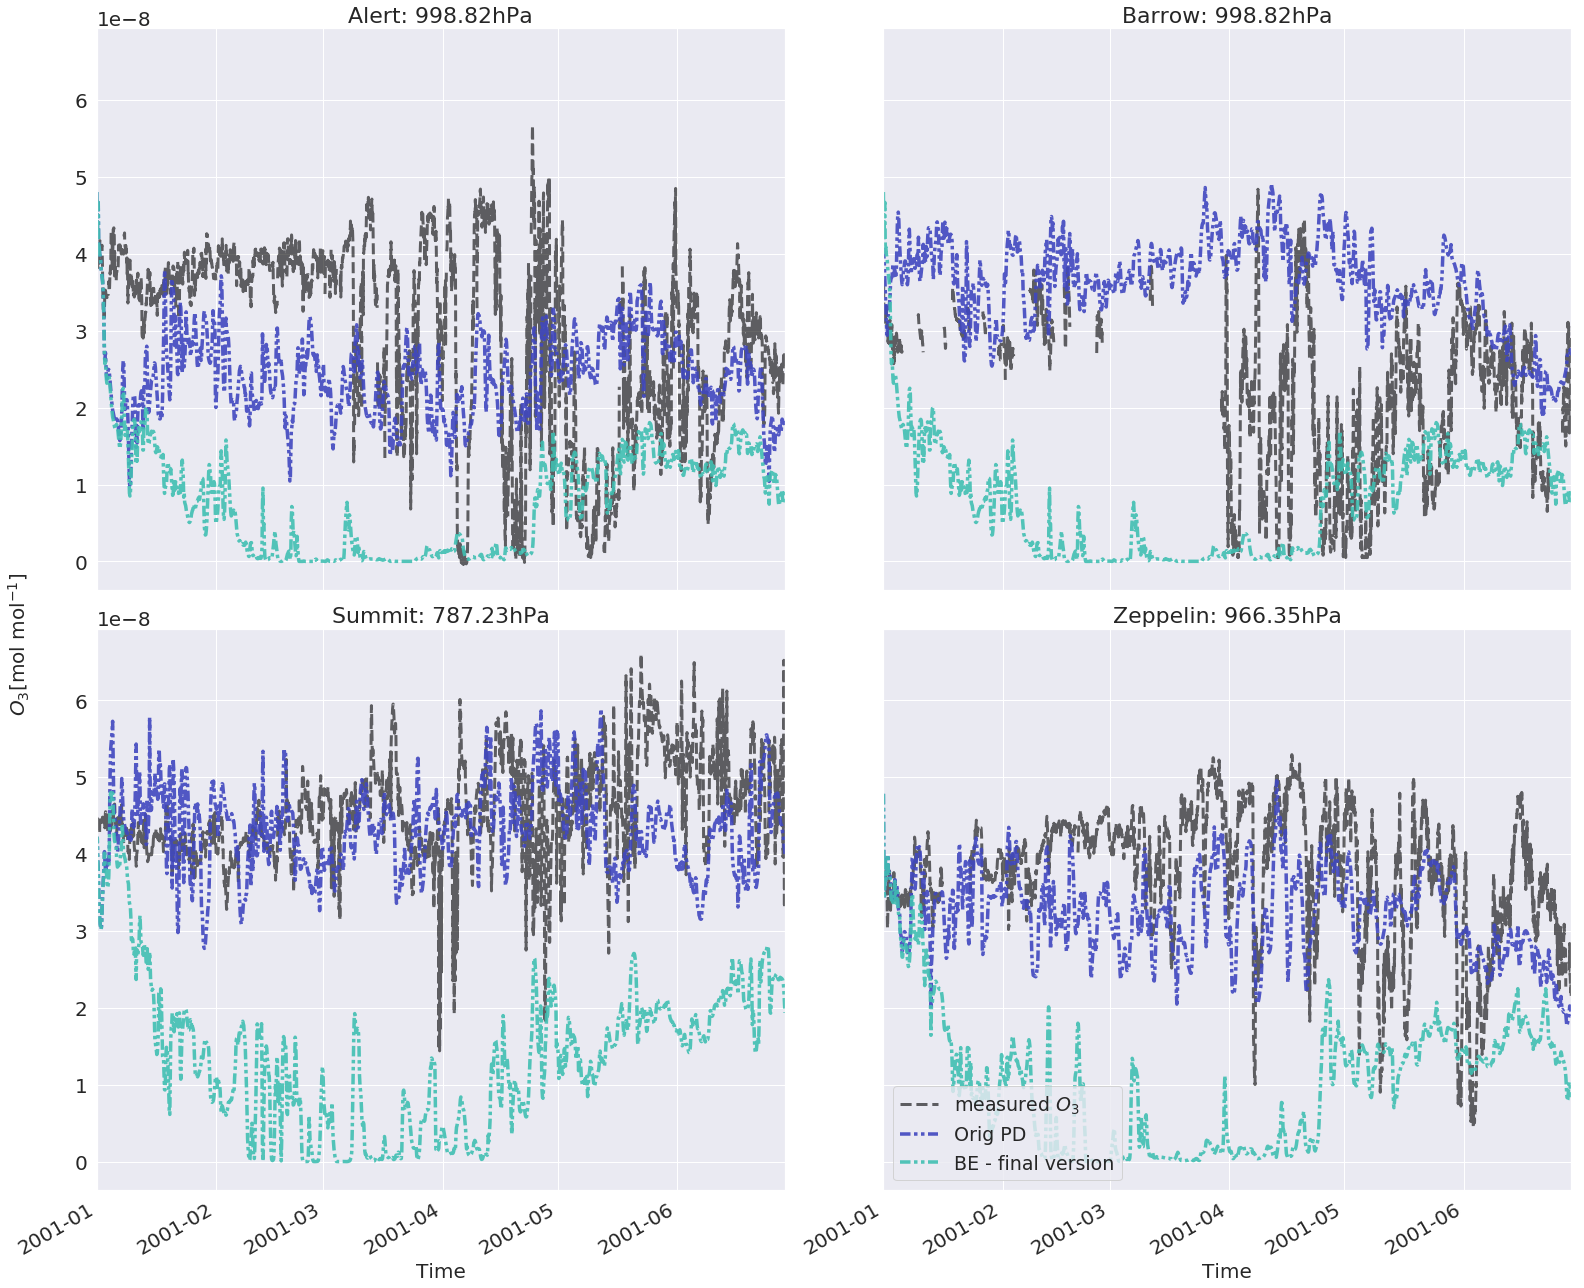
\includegraphics[width = \linewidth]{Chapter6_Results/images/ozone_2001_step5.png}
    \caption{Ozone measurements (black line) and model results from the original CTM3 (Branch \ref{def:origCTM3_PD}) (blue line) and the final version of the halogen branch (turquoise line) at the four different stations, Alert (top left), Barrow (top right), Summit (lower left) and Zeppelin (lower right) with available measurements in 2001. Model results were taken from the approximate altitude of the station in hPa. PD = present day, BE = bromine explosion}
    \label{fig:step5}
\end{figure}
\begin{figure}[h]
    \centering
    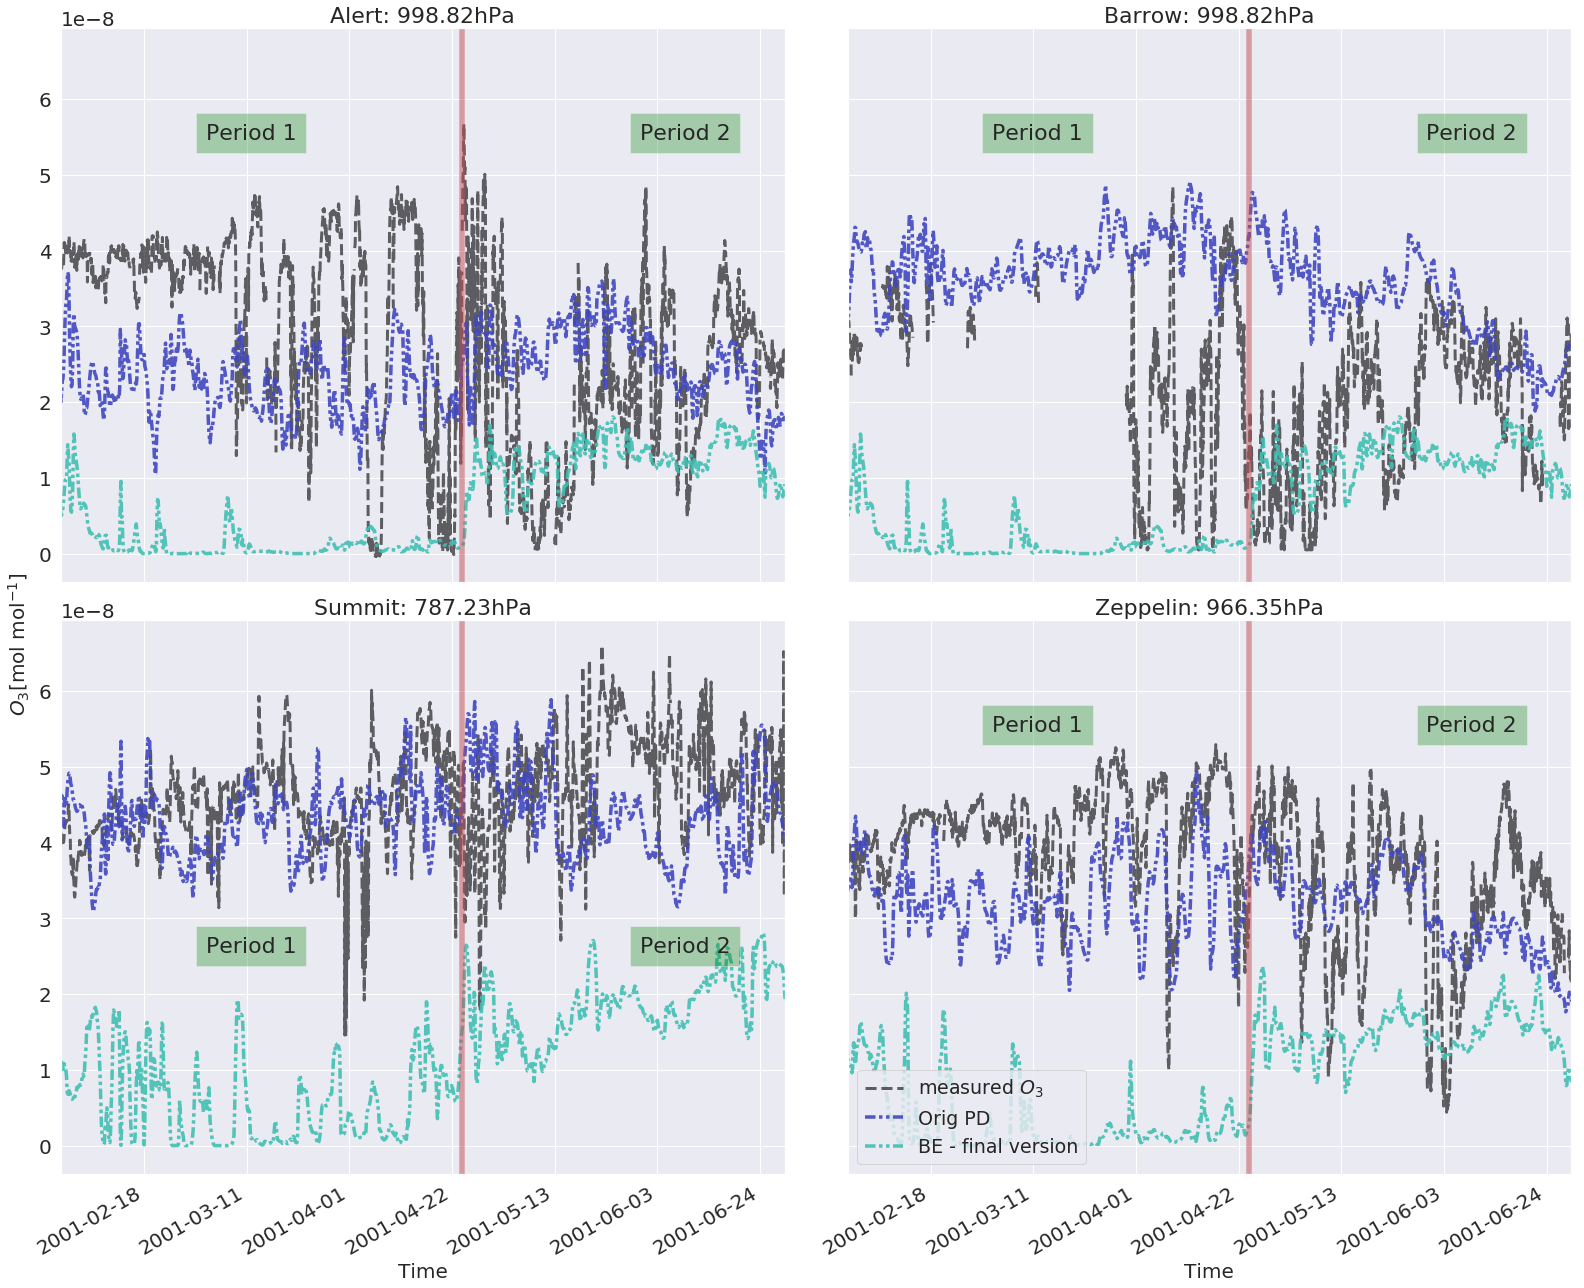
\includegraphics[width = \linewidth]{Chapter6_Results/images/ozone_stationComp_2001/ozone_2001_2periods_step5.png}
    \caption{Ozone measurements (black line) and model results from the original CTM3 (Branch \ref{def:origCTM3_PD}) (blue line) and the final version of the halogen branch (turquoise line) at the four different stations, Alert (top left), Barrow (top right), Summit (lower left) and Zeppelin (lower right) with measurements and model results from February to June, 2001. The results are split into two periods, 'Period 1' and 'Period 2'. Model results were taken from the approximate altitude of the station in hPa. PD = present day, BE = bromine explosion}
    \label{fig:2p_step5}
\end{figure}

\medskip

Figures \ref{fig:vert_ALT}-\ref{fig:vert_ZEP} contains the temporal evolution of ozone and halogen species in the model layers above Alert, Barrow, Zeppelin and Summit, respectively. It can be seen from all figures that there is a clear distinction between Period 1 and Period 2, with increased ozone mixing ratios in Period 2, also with altitude. 

\medskip

At Alert (Figure \ref{fig:vert_ALT}), the distinction between Period 1 and 2 considering ozone is an increase from approximately 0-8 ppb in Period 1 to 10-30 ppb in Period 2, with the highest levels found aloft. From the end of April (in Period 1) until the end of May (in Period 2), the \chem{HBr} mixing ratio is on average approximately 10-30 ppt, with a peak in the separation between the two period (around the 24th of April). This behaviour of the temporal evolution of \chem{HBr} can be seen in Figures \ref{fig:vert_BRW}-\ref{fig:vert_ZEP} as well. The other halogen species generally have a low mixing ratio in Period 1, and are virtually non-existent in Period 2. 

\medskip

The ozone mixing ratio at Barrow (in Figure \ref{fig:vert_BRW}) in Period 1 is approximately 6-20 ppb, and increases to about 20-30 ppb in Period 2. Unlike the \chem{HOBr} mixing ratio seen at Alert, there is some increase in the mixing ratio during Period 2, however less than what's seen in Period 1. This also applies to the \chem{HOBr} mixing ratio seen at Summit (Figure \ref{fig:vert_SUM}) and Zeppelin (Figure \ref{fig:vert_ZEP}). The temporal evolution of the mixing ratio in the other halogen species results in virtually nothing in Period 2.

\medskip

At Summit (Figure \ref{fig:vert_SUM}), the ozone mixing ratio in Period 1 is low at the ground level (keep in mind that Summit station is located at 3238 m.a.s.l.). However, distinctly higher mixing ratios (30 - 40 ppb) can be seen aloft. In Period 2, the ground level ozone has increased a bit (up to about 15 ppb), but still with higher mixing ratios aloft. Differently from the other stations, \chem{BrCl} from aloft extends into Period 2, but dissappears mid-May.

\medskip

Lastly, the ozone mixing ratio at Zeppelin (Figure \ref{fig:vert_ZEP}) is quite low during Period 1 (approximately 0-10 ppb), and increases abruptly in Period 2 (up to about 20-40 ppb). 


\begin{figure}[h]
    \centering
    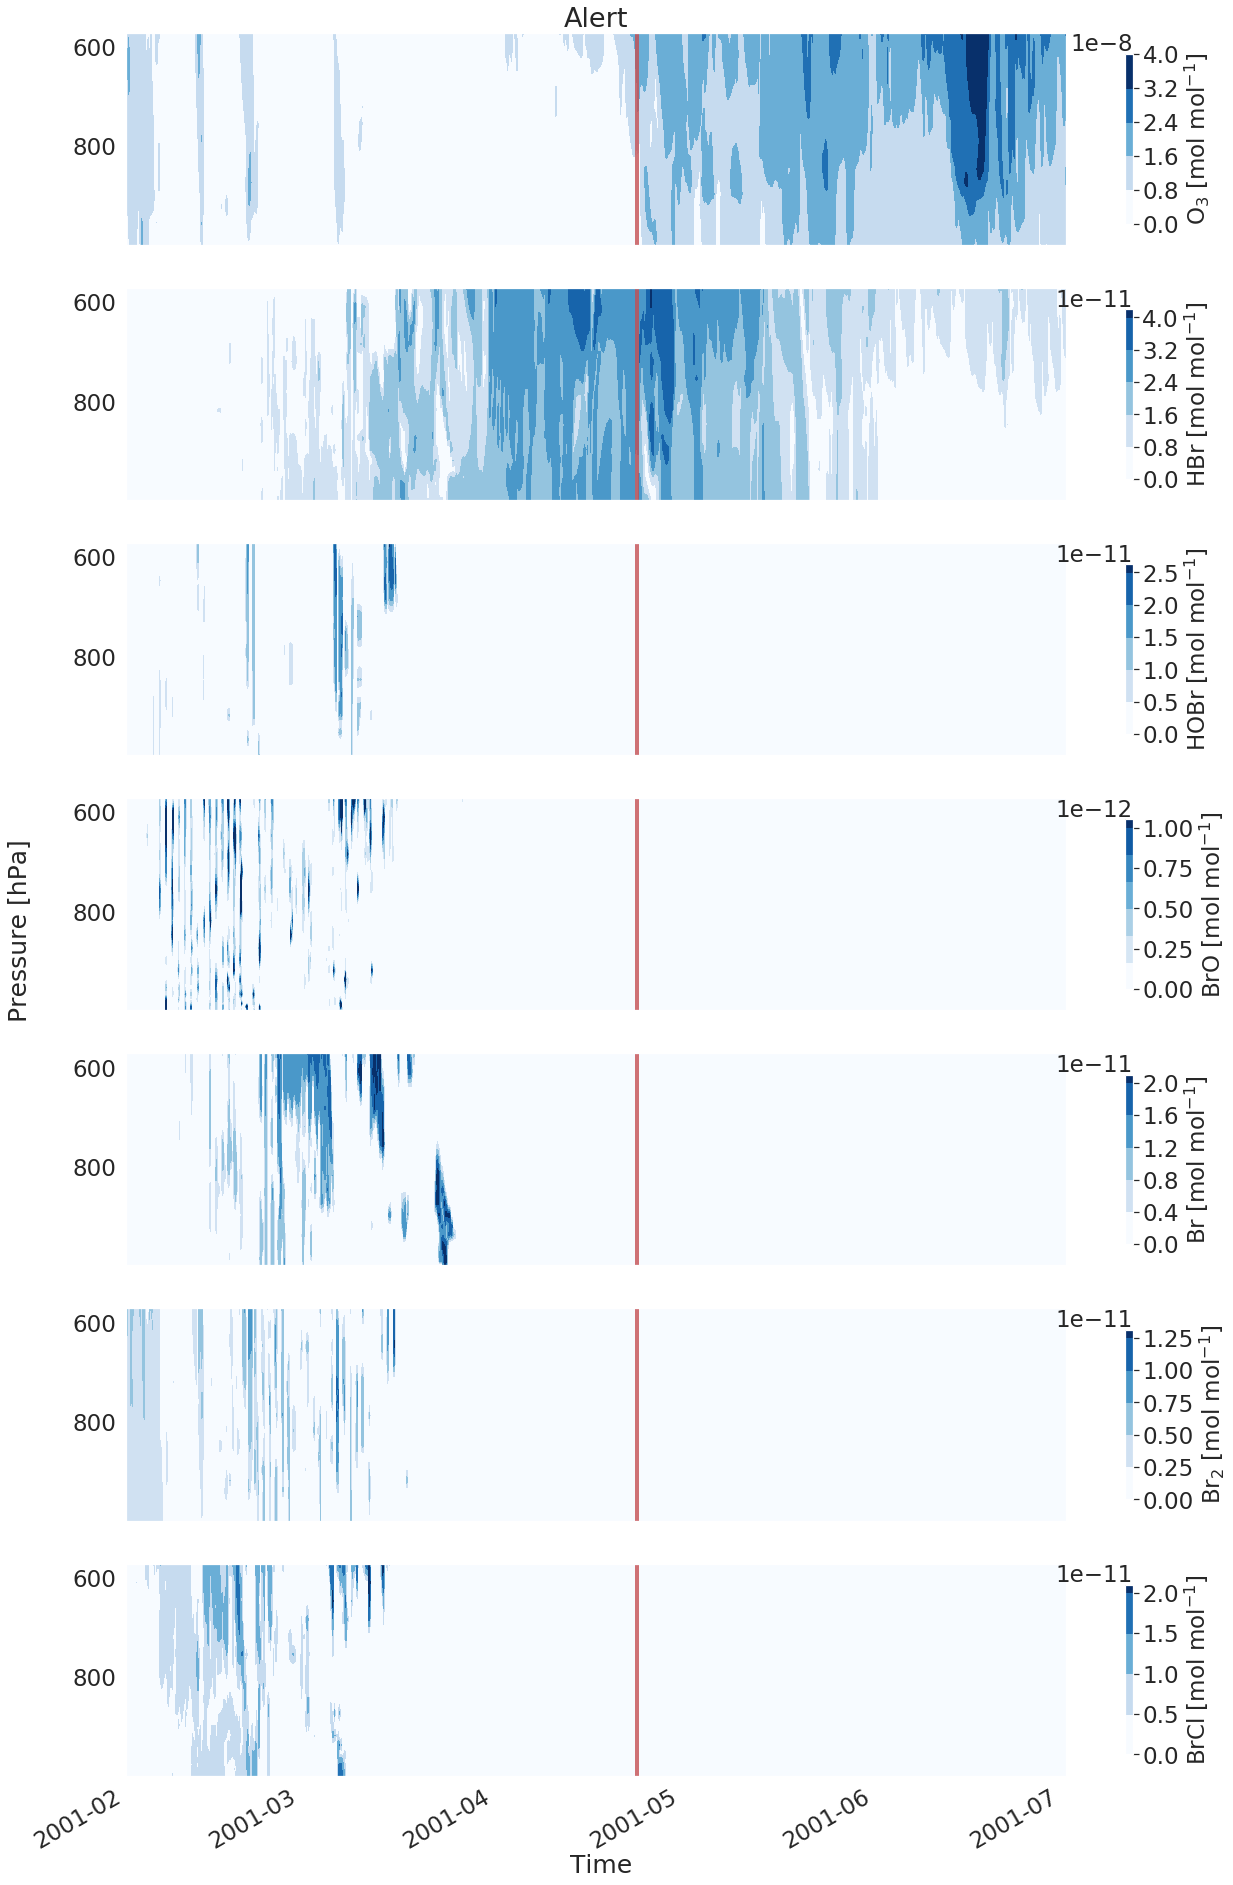
\includegraphics[width=\linewidth]{Chapter6_Results/images/Vert_StationComp_2001/vert_all_species_ALT.png}
    \caption{Mixing ratio ($mol mol^{-1}$) of $\chem{O_3}$, $\chem{HBr}$, $\chem{HOBr}$, $\chem{BrO}$,$\chem{Br}$ and $\chem{Br_2}$ from the station ground level up to $\sim 600 hPa$ at Alert in Period 1 (left of the red line) and Period 2 (right of the red line) in 2001}
    \label{fig:vert_ALT}
\end{figure}
\begin{figure}[h]
    \centering
    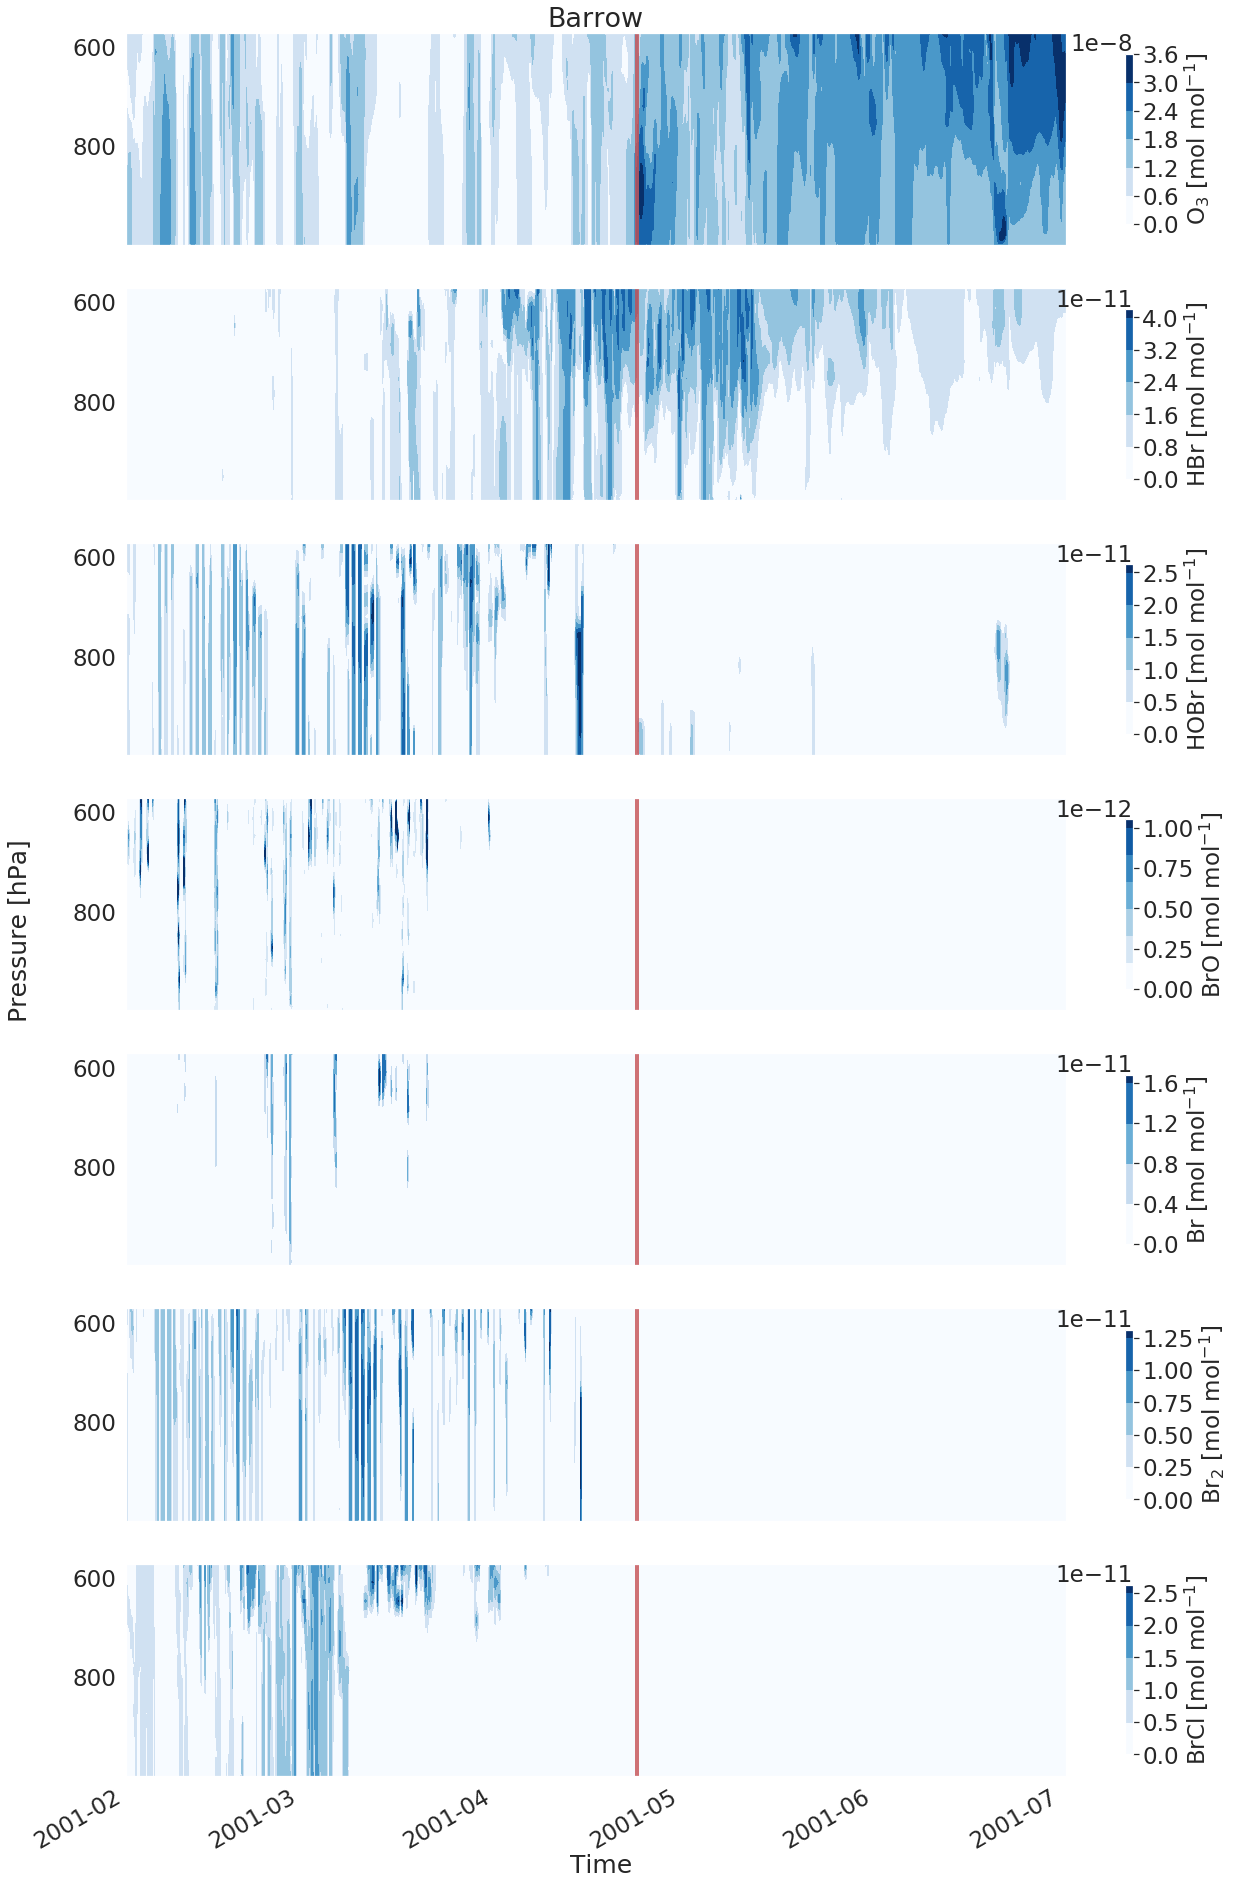
\includegraphics[width=\linewidth]{Chapter6_Results/images/Vert_StationComp_2001/vert_all_species_BRW.png}
    \caption{Mixing ratio ($mol mol^{-1}$) of $\chem{O_3}$, $\chem{HBr}$, $\chem{HOBr}$, $\chem{BrO}$,$\chem{Br}$ and $\chem{Br_2}$ from the station ground level up to $\sim 600 hPa$ at Barrow in Period 1 (left of the red line) and Period 2 (right of the red line) in 2001}
    \label{fig:vert_BRW}
\end{figure}
\begin{figure}[h]
    \centering
    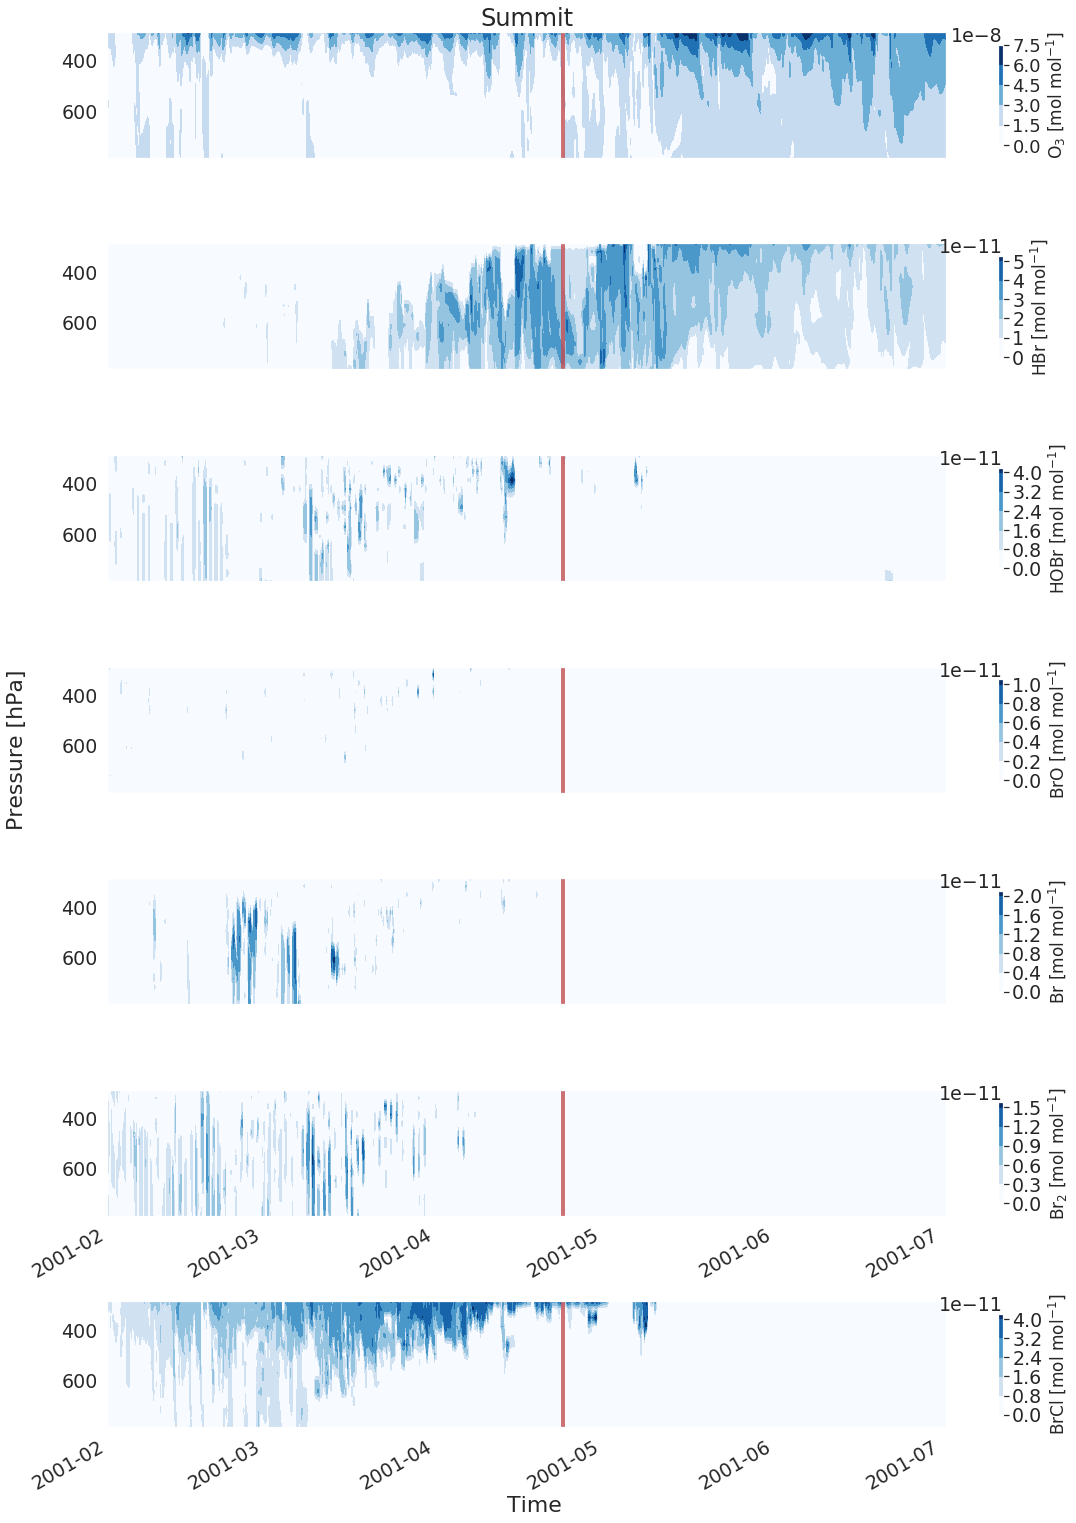
\includegraphics[width=\linewidth]{Chapter6_Results/images/Vert_StationComp_2001/vert_all_species_SUM.png}
    \caption{Mixing ratio ($mol mol^{-1}$) of $\chem{O_3}$, $\chem{HBr}$, $\chem{HOBr}$, $\chem{BrO}$,$\chem{Br}$ and $\chem{Br_2}$ from the station ground level up to $\sim 400 hPa$ at Summit in Period 1 (left of the red line) and Period 2 (right of the red line) in 2001}
    \label{fig:vert_SUM}
\end{figure}
\begin{figure}[h]
    \centering
    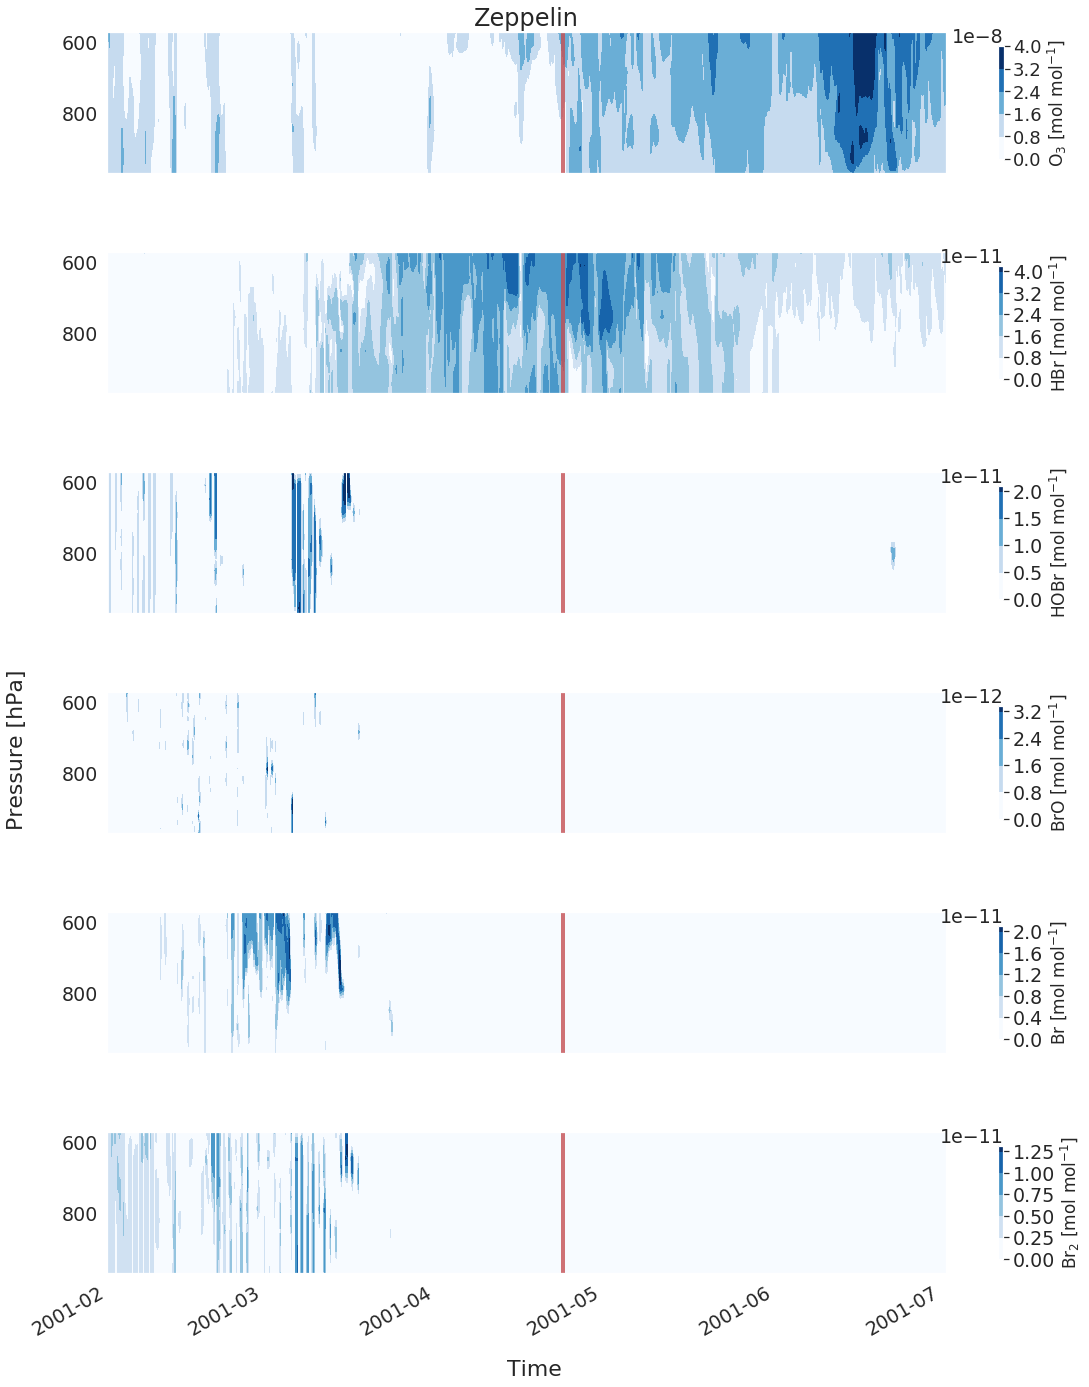
\includegraphics[width=\linewidth]{Chapter6_Results/images/Vert_StationComp_2001/vert_all_species_ZEP.png}
    \caption{Mixing ratio ($mol mol^{-1}$) of $\chem{O_3}$, $\chem{HBr}$, $\chem{HOBr}$, $\chem{BrO}$,$\chem{Br}$ and $\chem{Br_2}$ from the station ground level up to $\sim 600 hPa$ at Zeppelin in Period 1 (left of the red line) and Period 2 (right of the red line) in 2001}
    \label{fig:vert_ZEP}
\end{figure}


\clearpage

\subsection{Analysis of the Difference Between the Final BE-Branch and the Original CTM3}\label{sec:res_origBE} 

Figures \ref{fig:joint_FebApr_ALTSUM}- \ref{fig:joint_AprMay_ZEPBRW} contains distributions of the agreements between the original CTM3, the BE-branch and the observational data. They are divided into Period 1 and 2 to separate the BE-branch results before stabilization and after (before and after the 24th of April). The figures also show a distribution of the BE-branch- and Original CTM3-results as well as the distribution of the observed ozone. In addition, the Pearson correlation coefficient and corresponding p-value is shown\footnote{The Pearson correlation coefficient takes a values between $-1$ (exact linear negatively correlated relationship) and $1$ (exact linear positively correlated relationship). The p-value indicates the probability of an uncorrelated system producing datasets that have a Pearson correlation at least as extreme as the one computed from these datasets (statistically significant if $p<0.05$) (\cite{WILKS201123})}.

\medskip

Figure \ref{fig:joint_FebApr_ALTSUM} contains the distributions and correlations for Alert (ALT) and Summit (SUM) during Period 1. The resulting correlations between the model results and observation are poor and varies between being positively and negatively correlated. The highest correlation with observations is with the original CTM3-results at Alert (Pearson number $=0.16$, $p = 0.00011$) (lower right). Similarly, the correlations shown in Figure \ref{fig:joint_FebApr_ZEPBRW}, for Zeppelin (ZEP) and Barrow (BRW), are poor and varies between being positively and negatively correlated. Again, the highest correlation with observations is with the original CTM3-results at Zeppelin (Pearson number $=0.43$, $p = 9.81\times10^{-31}$) (upper right). 

\medskip

In Period 2, the distribution of the BE-branch and Original CTM3 against observations at Alert and Summit are shown in Figure \ref{fig:joint_AprMay_ALTSUM}. Again, the correlations are somewhat poor. The highest correlation with observations is with the BE-branch at Alert (Pearson number $=0.33$, $p = 7.8\times10^{-14}$) (lower left). However, at Zeppelin (in Figure \ref{fig:joint_AprMay_ZEPBRW}), the highest correlation is found between the observations and the Original CTM3 (Pearson number $=0.5$, $p = 1.7\times10^{-34}$) (upper right). 



\begin{figure}[ht]
    \centering
    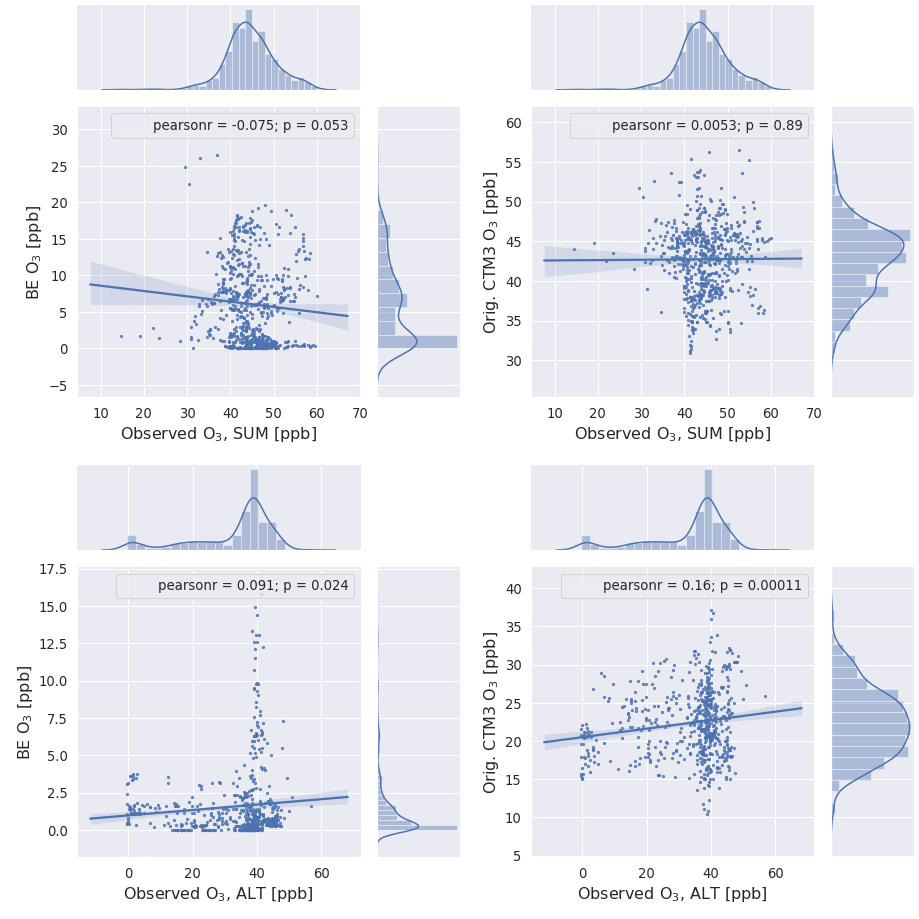
\includegraphics[width = \linewidth]{Chapter6_Results/images/Orig_BE_comp/jointplot_FebApr_ALTSUM_O3_2001.png}
    \caption{Measured $\chem{O_3}$ in ppb vs. modelled results from the and modelled results from the BE-branch (left columns) and original CTM3 (right columns) at  Alert (ALT) (top) and Summit (SUM) (bottom) (model results taken from the station's approximate altitude). The histogram distribution of the observations (x-axis) and the model results (y-axis) are shown on the x- and y-axis, respectively. The Pearson correlation coefficient and p-value is shown in the top right corner. \textbf{Period 1} - February 1st-April 24th, 2001}
    \label{fig:joint_FebApr_ALTSUM}
\end{figure}


\begin{figure}[ht]
    \centering
    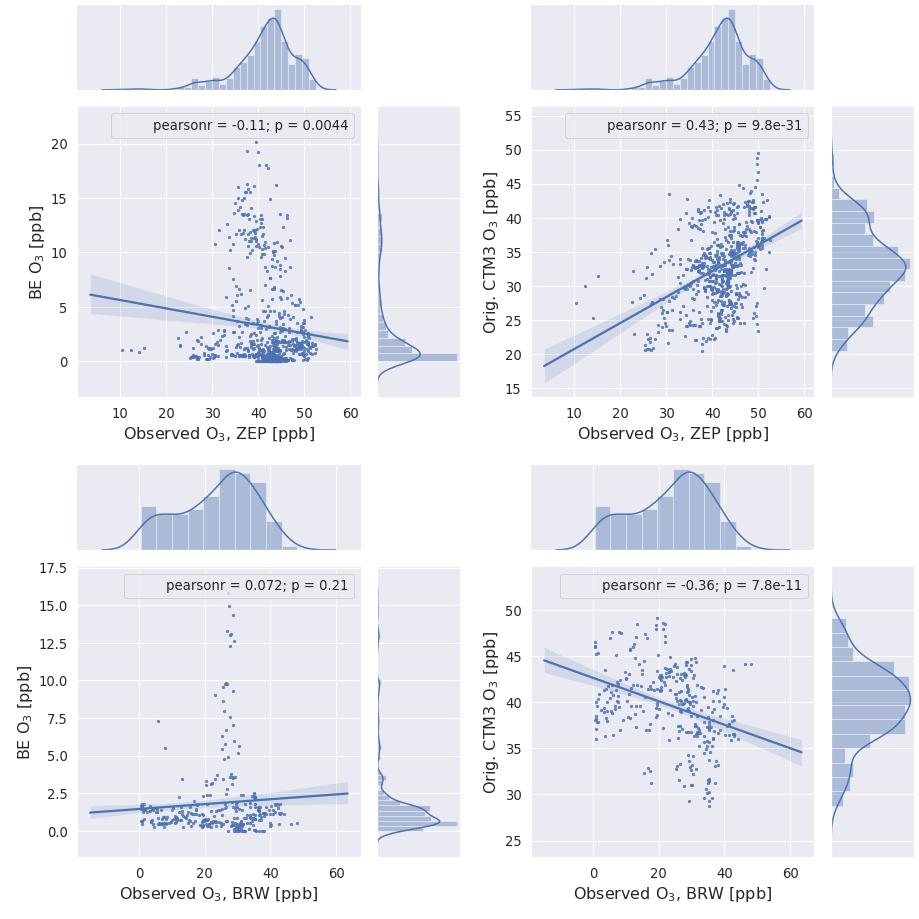
\includegraphics[width = \linewidth]{Chapter6_Results/images/Orig_BE_comp/jointplot_FebApr_ZEPBRW_O3_2001.png}
    \caption{Measured $\chem{O_3}$ in ppb vs. modelled results from the and modelled results from the BE-branch (left columns) and original CTM3 (right columns) at  Zeppelin (ZEP) (top) and Barrow (BRW) (bottom) (model results taken from the station's approximate altitude) The histogram distribution of the observations (x-axis) and the model results (y-axis) are shown on the x- and y-axis, respectively. The Pearson correlation coefficient and p-value is shown in the top right corner. \textbf{Period 1} - February 1st-April 24th, 2001}
    \label{fig:joint_FebApr_ZEPBRW}
\end{figure}

\begin{figure}[ht]
    \centering
    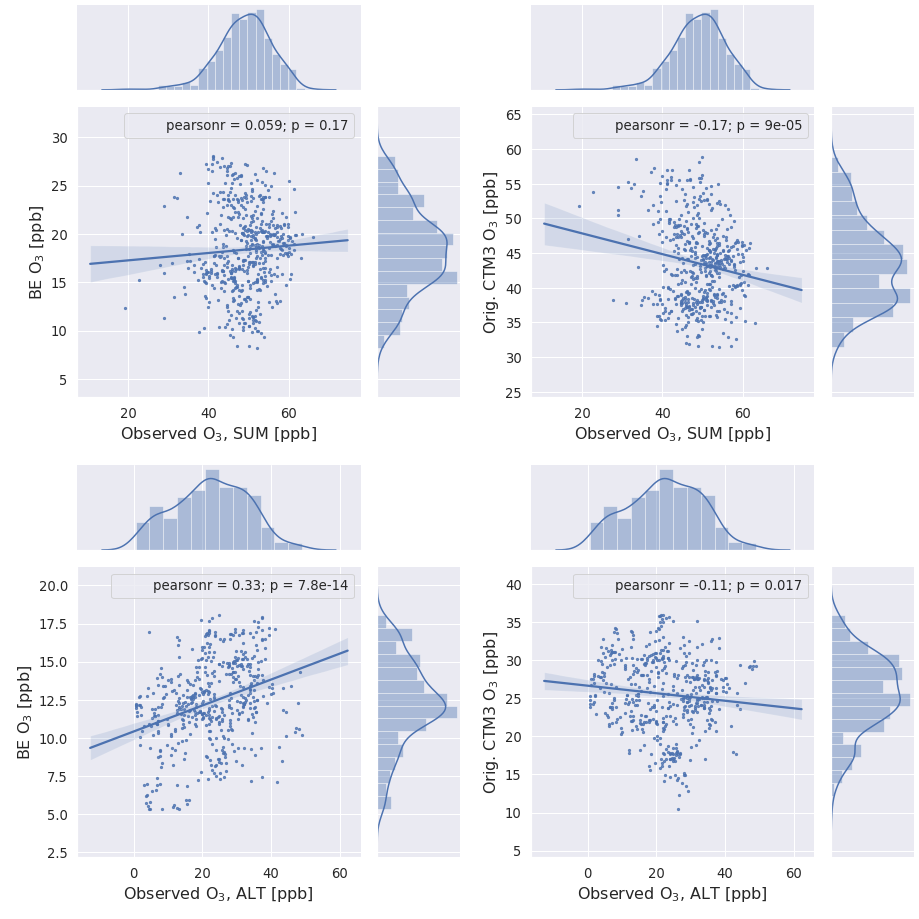
\includegraphics[width = \linewidth]{Chapter6_Results/images/Orig_BE_comp/jointplot_AprJune_ALTSUM_O3_2001.png}
    \caption{Measured $\chem{O_3}$ in ppb vs. modelled results from the and modelled results from the BE-branch (left columns) and original CTM3 (right columns) at Summit (SUM) (top) and Alert (ALT) (bottom) (model results taken from the station's approximate altitude). The histogram distribution of the observations (x-axis) and the model results (y-axis) are shown on the x- and y-axis, respectively. The Pearson correlation coefficient and p-value is shown in the top right corner. \textbf{Period 2} - April 24th-June 30th, 2001}
    \label{fig:joint_AprMay_ALTSUM}
\end{figure}

\begin{figure}[ht]
    \centering
    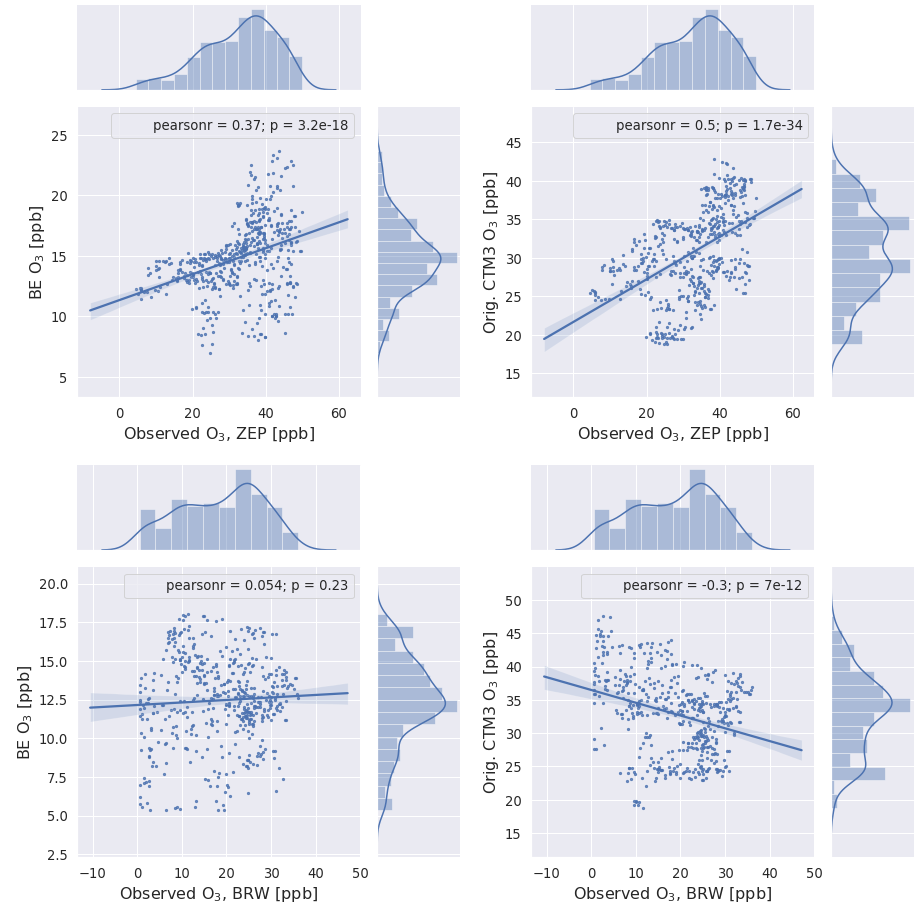
\includegraphics[width = \linewidth]{Chapter6_Results/images/Orig_BE_comp/jointplot_AprJune_ZEPBRW_O3_2001.png}
    \caption{Measured $\chem{O_3}$ in ppb vs. modelled results from the and modelled results from the BE-branch (left columns) and original CTM3 (right columns) at  Zeppelin(ZEP) (top) and Barrow(BRW) (bottom) (model results taken from the station's approximate altitude). The histogram distribution of the observations (x-axis) and the model results (y-axis) are shown on the x- and y-axis, respectively. The Pearson correlation coefficient and p-value is shown in the top right corner. \textbf{Period 2} - April 24th-June 30th, 2001}
    \label{fig:joint_AprMay_ZEPBRW}
\end{figure}

\medskip
\medskip

Figures \ref{fig:BE_origPD_vmrperc_FebApr} - \ref{fig:BE_origPD_vmrperc_AprJune} shows the monthly mean mixing ratio (in ppb) in the first model layer, where the BE-branch results are subtracted from the CTM3-branch (left columns) and the percentage difference between the CTM3-branch and the BE-branch in the Arctic (above 68$^o$N) for Period 1 (February-April) and Period 2 (April-June) in 2001. \footnote{For global figures, see Appendix \ref{app:final_version}. Figures \ref{fig:BE_origPD_vmr_lev0_FebApr}-\ref{fig:BE_origPD_vmr_lev0_AprJun} contains the global difference (Original CTM3 - BE-branch) in mixing ratio, and Figures \ref{fig:BE_origPD_percent_FebApr}-\ref{fig:BE_origPD_percent_AprJun} contains the percentage difference.} Figure \ref{fig:BE_origPD_vmrperc_FebApr} contains the results from Period 1. From the mixing ratio column, it is evident that the Original CTM3 produces higher mixing ratios than the BE-branch in general, with an exception in Northern Canada in February (top row). The percentage difference shows that in February, the Original CTM3 more or less produces about 120\% higher ozone mixing ratios over Greenland, parts of Svalbard and over the ocean. The monthly means in March and April shows that the BE-branch produce lower mixing ratios in the first model layer than the Original CTM3. The percentage difference is above 100\% in March, and is maximum 96 \% in April over the ocean.

\medskip

In Figure \ref{fig:BE_origPD_vmrperc_AprJune}, the monthly mean difference in mixing ratio and percentage difference is drawn for Period 2. Over the course of these months, the difference between the Original CTM3 and the BE-branch both in mixing ratio and percentage difference decreases. In June, the highest percentage difference can be seen over Greenland and over the ocean towards the Bering Strait (lower right).


\begin{figure}[h]
    \centering
    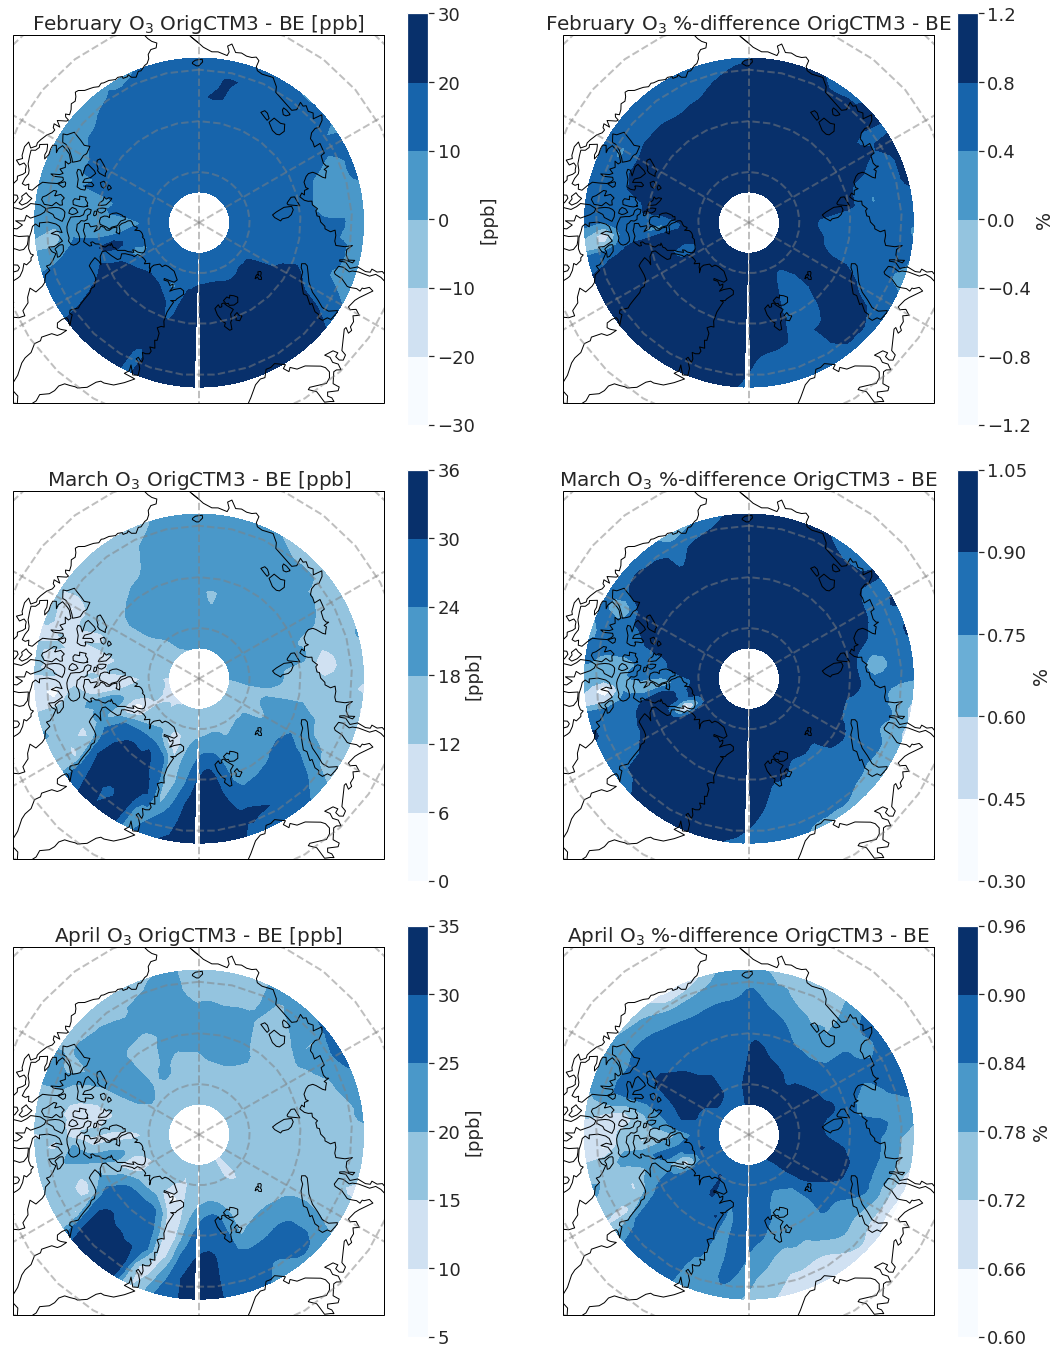
\includegraphics[width = \linewidth]{Chapter6_Results/images/Orig_BE_comp/polar_VMRperc_FebApr_2001.png}
    \caption{Difference in ozone monthly mean volume mixing ratio (in ppb) (left columns) and percentage difference (right columns) in the first model layer between the original CTM3 and the BE-branch globally (left columns) and in the Arctic (right columns) in the months February (top figures), March (middle figures) and April (bottom figures) in 2001. \textbf{Note:} the colorbar axis are not equal}
    \label{fig:BE_origPD_vmrperc_FebApr}
\end{figure}
\begin{figure}[h]
    \centering
    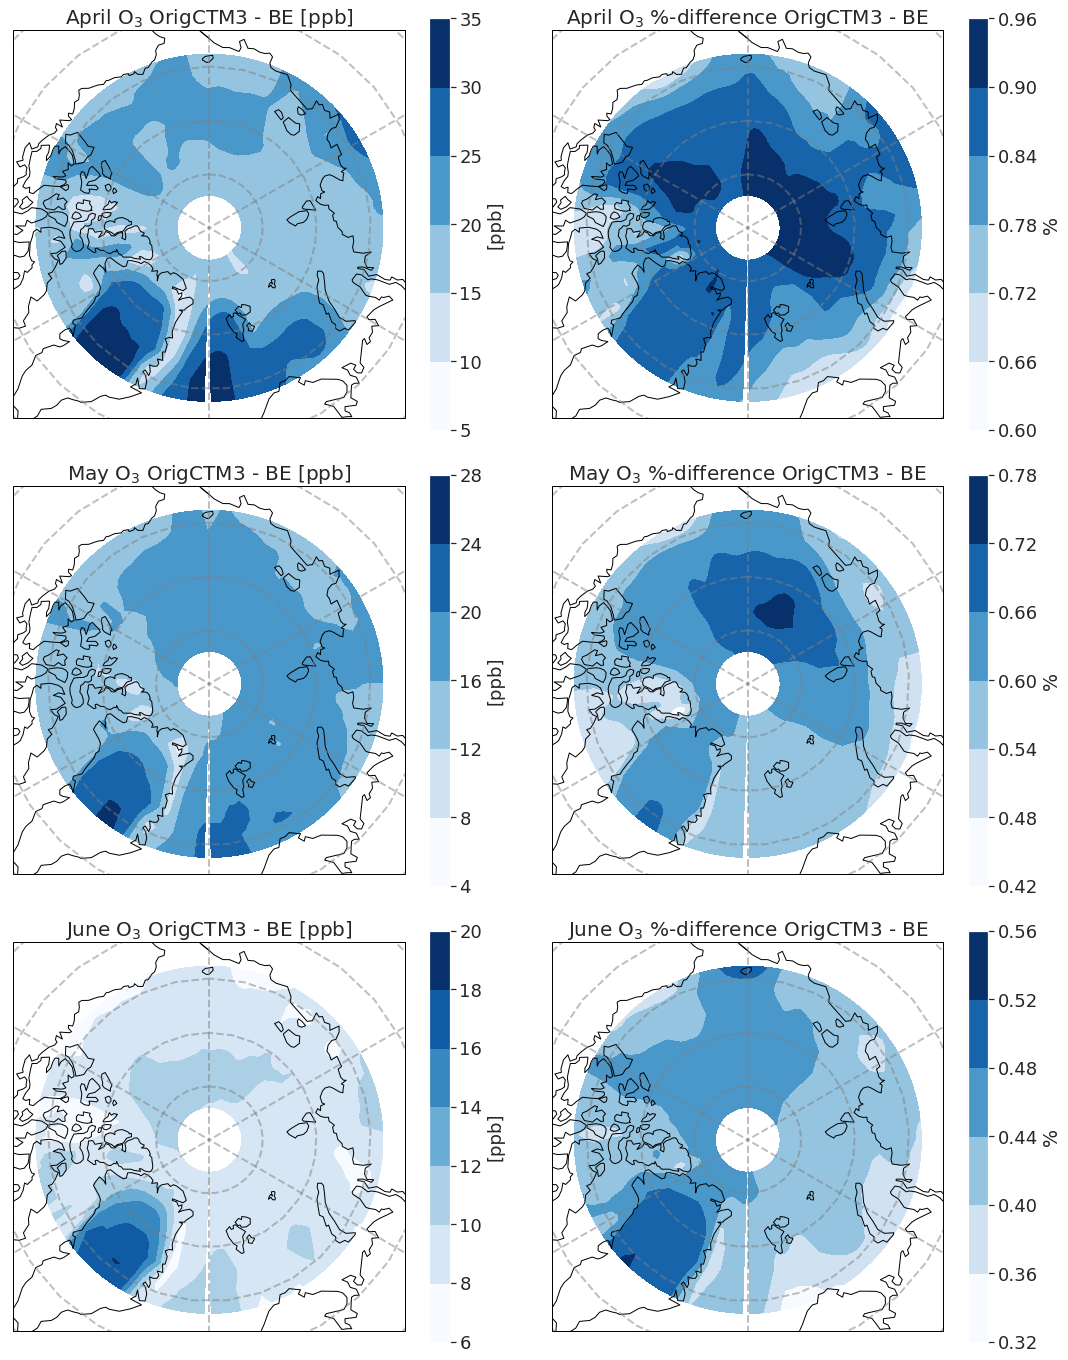
\includegraphics[width = \linewidth]{Chapter6_Results/images/Orig_BE_comp/polar_VMRperc_AprJune_2001.png}
    \caption{Ozone monthly mean volume mixing ratio (in ppb) from the BE-branch (left columns) and from the Original CTM3 (middle columns) and the difference (Original CTM3-BE-branch) (right columns) in the months April (top figures), May (middle figures) and June (bottom figures) in 2001. \textbf{Note:} the colorbar axis are not equal}
    \label{fig:BE_origPD_vmrperc_AprJune}
\end{figure}
%\section{Comparison with literature}

%\cite{Zhao2016} measured BrO column at Eureka in 2011 -- SJekk ut! 


%\cite{Peterson2016} and \cite{Peterson2015} -- BrO over Barrow -- sjekk ut! 

%Measurements of $\chem{Br_2}$, \chem{BrCl} and $\chem{O_3}$ were conducted by \cite{Foster2001} at Alert research station. They found $\chem{Br_2}$ mixing ratios up to $\sim$ 25 \acrshort{ppt} and \chem{BrCl} at mixing ratios up to 35 \acrshort{ppt} between day 40 and 75 in 2001. Ozone was depleted from background values of $\sim$ 30-40 \acrshort{ppb} to below 10 ppb. 

%\medskip

%\cite{Simpson2017} investigated the \chem{BrO} column using \acrlong{maxdoas} instrumentation near Barrow in 2012.

%\medskip

%\cite{Luo2018} also investigated the \chem{BrO} column using \acrshort{maxdoas} in Ny Ålesund in 2015. 

%\medskip

%\cite{Thomas2012} and \cite{Thomas2011} about the mechanism behind ODEs at Summit, Greenland. 

%\section{Calculation of radiative forcing using PD- and PI model results}
\clearpage
\section{Radiative forcing}\label{sec:res_RF}

The radiative forcing was calculated by running both the BE-branch and the Original CTM3 with a \acrlong{pd}-setup, and a \acrlong{pi}-setup (for the year 1850). The monthly averaged ozone concentration (in gm$^{-3}$) was converted to \acrlong{du} (in each model layer up to the model tropopause). The concentration in DU was then multiplied with a normalized RF-field (in mWm$^{-2}$DU$^{-1}$) (provided by \cite{MariannePersonal}). Equation \ref{eqn:RF} sums up the calculation.

\begin{equation}
    RF_{\chem{O_3}} = (M_{PD} - M_{PI})*\text{netNRF}
    \label{eqn:RF}
\end{equation}

In which $RF_{\chem{O_3}}$ is the \acrshort{rf} due to ozone, $M_{PD}$ and $M_{PI}$ is the monthly averaged modelled ozone (in DU) for a present-day run and a pre-industrial run, respectively. The normalized RF-field contains both a short-wave and long-wave component, such that netNRF = SW + LW.

\medskip

\textbf{NOTE:} the BE-branch \acrshort{pd}- and \acrshort{pi}-runs were ran from different model setups. The Henry's law coefficient and photodissociation rates in the PD-run were set as in the final version (explained in Section \ref{sec:res_step4}) whereas the PI-run was set up with the values used in the previous version (\ref{sec:res_step3} with the high Henry's law constant). This became the solution as the model produced negative values of a radical (\texttt{ISOR1}) when the other setup was applied to the PD- and PI-branches. 

\medskip

Figures \ref{fig:BEorig_RF_global_FebApr_2001}-\ref{fig:BEorig_RF_global_AprJune_2001} contain the RF due to ozone in the whole tropospheric column calculated for the BE-branch (left columns) and the RF calculated by the Original CTM3 minus the RF by the BE-branch (right columns) in the Arctic\footnote{A figure containing the global RF produced by the BE-branch can be found in Appendix \ref{app:RF}, Figure \ref{fig:BE_RF_global_2001}, global and Arctic RF produced by the Original CTM3 can be found in Figures \ref{fig:origRF_global_2001}-\ref{fig:origRF_arctic_2001}, respectively}. 
\medskip 

Period 1 is shown in Figure \ref{fig:BEorig_RF_global_FebApr_2001}. The BE-branch ozone-induced RF (left columns) in February is quite homogeneous, and reads approximately $0-2.5\times10^{-5}$ Wm$^{-2}$ across the Arctic, and slightly higher over Svalbard and the Barents Sea. The difference in RF between the Original CTM3 and the BE-branch shows that the RF calculated by the BE-branch matches the one produced by the Original CTM3 around the poles. Through March, the BE-branch produces some negative RF north of Canada. The difference in RF between the Original CTM3 and the BE-branch produces zero RF over the Arctic ocean towards and over Greenland, but is otherwise positive. Through April, the BE-branch RF is zero or positive and the difference in RF between the Original CTM3 and the BE-branch is positive.

\medskip

Throughout Period 2 (in Figure \ref{fig:BEorig_RF_global_AprJune_2001}), the BE-branch RF increases, but the difference in RF between the Original CTM3 and the BE-branch produces solely positive values, meaning that the RF produced by the Original CTM3 is higher.

\medskip

The averaged RF globally and over the Arctic, produced by the BE-branch and the Original CTM and the difference between them for the whole period, Period 1 and Period 2 is shown in Table \ref{tab:RF_results}. The table exhibits large variations considering whether the BE-branch takes the whole atmosphere into account, or just the Arctic. Globally the BE-branch may produce negative RF (the whole time period and Period 2), but in the Arctic, the RF is always negative. Also, averaged over the Arctic and globally, the Original CTM3 produces a higher RF, which can be seen from the difference between the two branches. 

\medskip

\begin{figure}[ht]
    \centering
    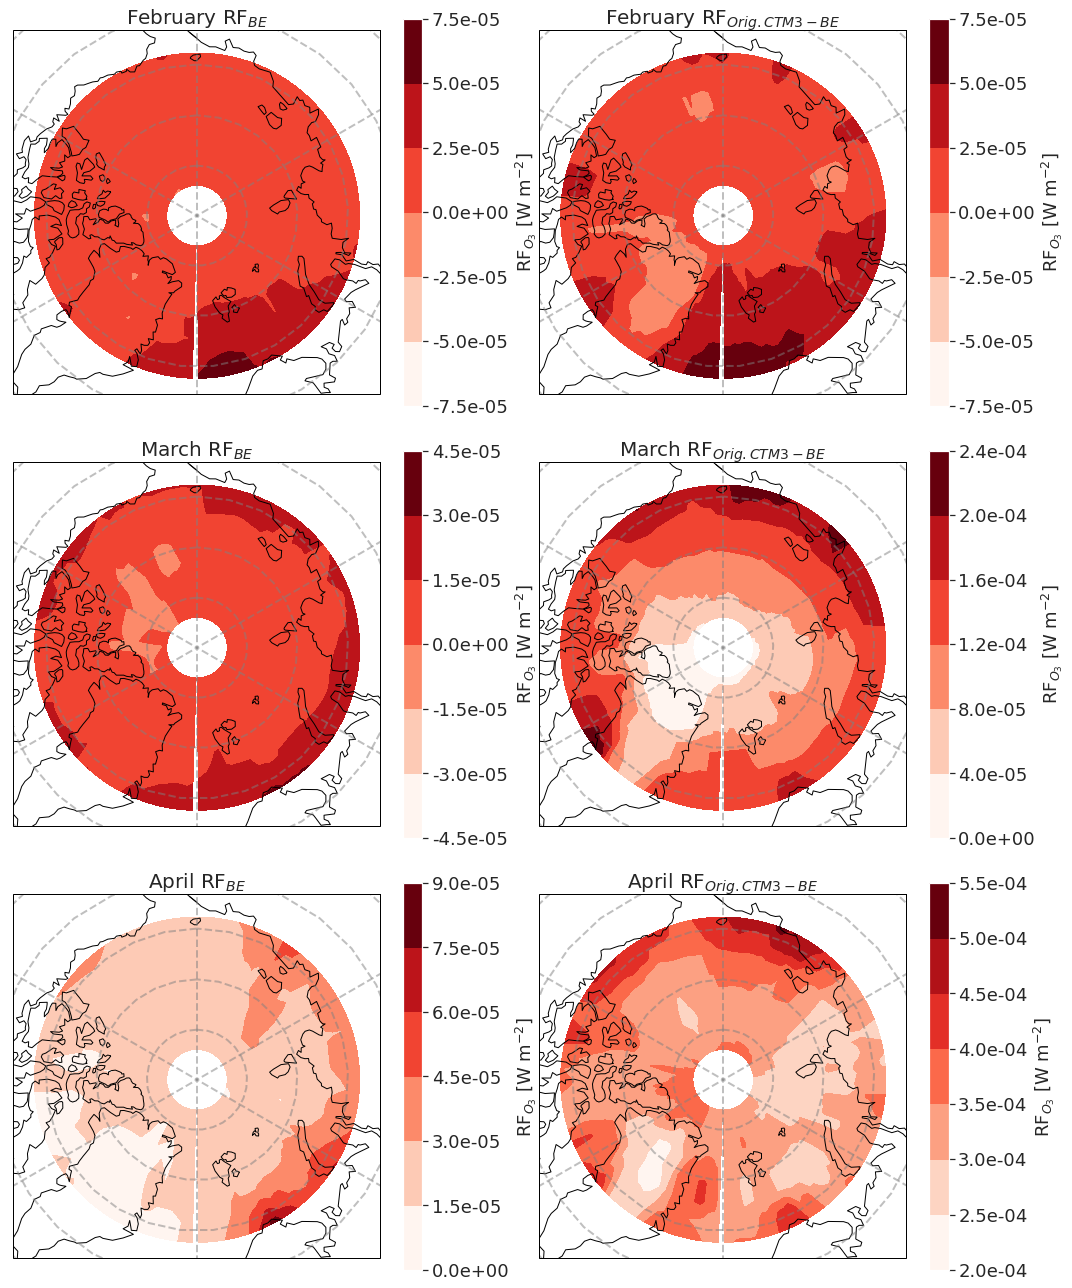
\includegraphics{Chapter6_Results/images/RF/BEOrig_RF_polar_FebApr_2001.png}
    \caption{Polar RF-field (in Wm$^{-2}$) for the total tropospheric column up to the tropopause, produced using the BE-branch (left columns) and the Orig. CTM3 RF minus the BE-branch RF (right columns) for the months February (top figures), March (middle figures) and April (bottom figures)}
    \label{fig:BE_RF_global_FebApr_2001}
\end{figure}
\begin{figure}[ht]
    \centering
    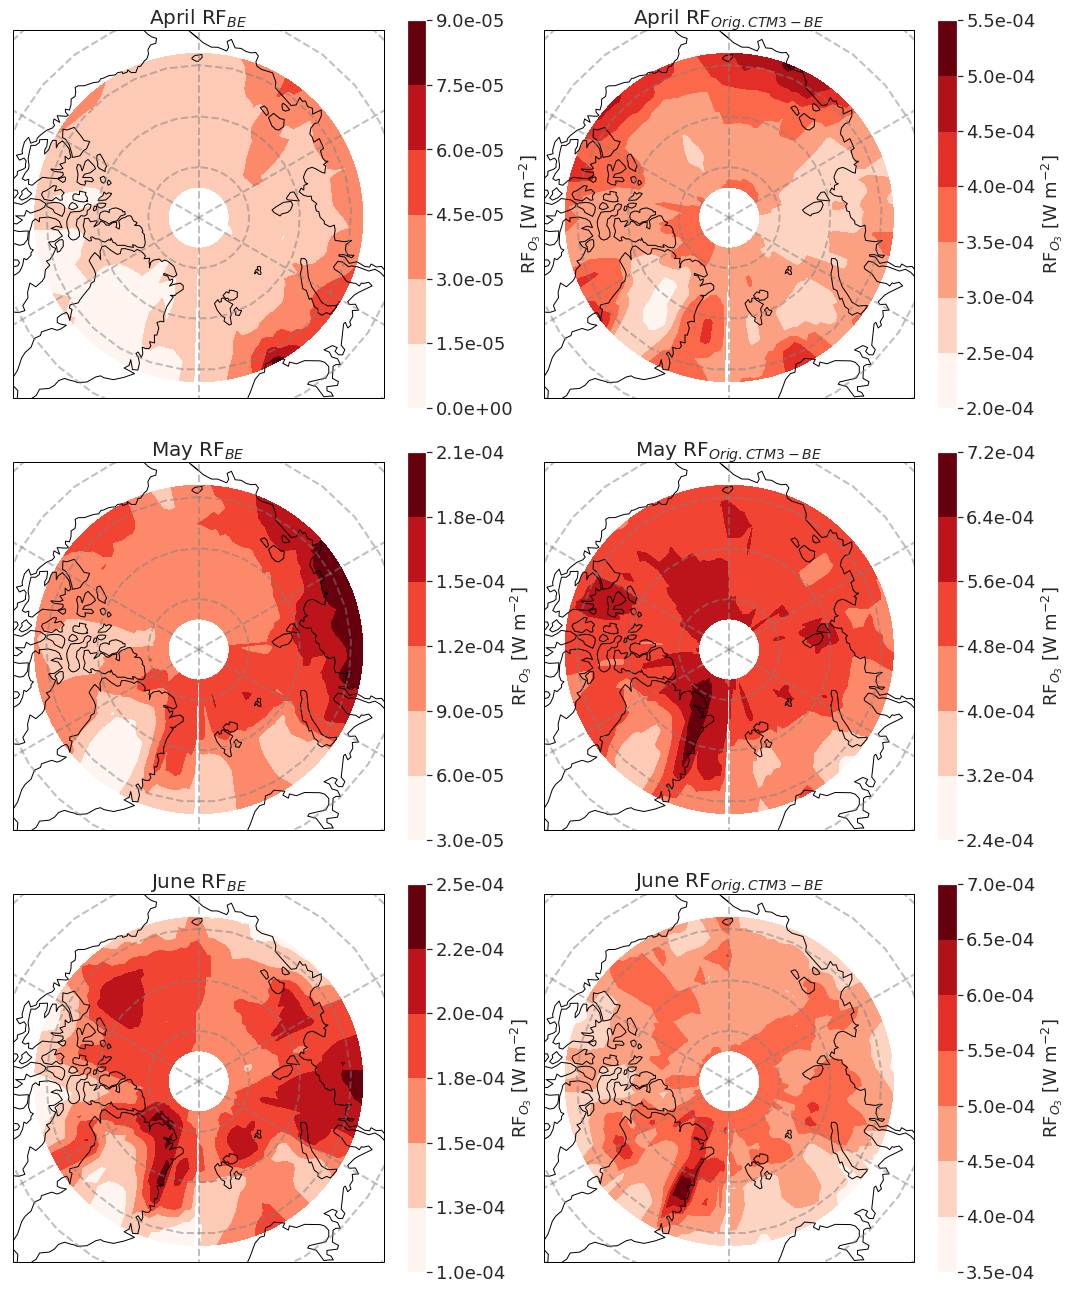
\includegraphics[width = \linewidth]{Chapter6_Results/images/RF/BEOrig_RF_polar_AprJune_2001.png}
    \caption{Polar RF-field (in Wm$^{-2}$) for the total tropospheric column up to the tropopause, produced using the BE-branch (left columns) and the Orig. CTM3 RF minus the BE-branch RF (right columns) for the months April (top figures), May (middle figures) and June (bottom figures)}
    \label{fig:BE_RF_global_AprJune_2001}
\end{figure}

\begin{table}[h]
\centering
\begin{tabular}{|l|c|c|}
\hline
\textbf{}                     & \multicolumn{1}{l|}{\textbf{Global {[}Wm$^{-2}${]}}} & \multicolumn{1}{l|}{\textbf{Arctic {[}Wm$^{-2}${]}}} \\ \hline
\multicolumn{3}{|c|}{\textbf{The whole time period}}                                                                                        \\ \hline
\textbf{RF - Orig. CTM3}      & $3.1\times10^{-4}\pm2.2\times10^{-4}$                & $2.8\times10^{-4}\pm2.4\times10^{-4}$                \\
\textbf{RF - BE}              & $-1.1\times10^{-5}\pm1.1\times10^{-4}$               & $3.8\times10^{-5}\pm4.6\times10^{-5}$                \\
\textbf{RF (Orig. CTM3 - BE)} & $3.2\times10^{-4}\pm2.6\times10^{-4}$                & $2.4\times10^{-4}\pm2.0\times10^{-4}$                \\ \hline
\multicolumn{3}{|c|}{\textbf{Period 1}}                                                                                                     \\ \hline
\textbf{RF - Orig. CTM3}      & $2.6\times10^{-4}\pm1.6\times10^{-4}$                & $6.6\times10^{-5}\pm5.7\times10^{-5}$                \\
\textbf{RF - BE}              & $2.7\times10^{-5}\pm7.8\times10^{-5}$                & $9.5\times10^{-6}\pm9.6\times10^{-6}$                \\
\textbf{RF (Orig. CTM3 - BE)} & $2.3\times10^{-4}\pm1.9\times10^{-4}$                & $5.7\times10^{-5}\pm5.4\times10^{-5}$                \\ \hline
\multicolumn{3}{|c|}{\textbf{Period 2}}                                                                                                     \\ \hline
\textbf{RF - Orig. CTM3}      & $3.5\times10^{-4}\pm2.5\times10^{-4}$                & $4.9\times10^{-4}\pm1.5\times10^{-4}$                \\
\textbf{RF - BE}              & $-5.0\times10^{-5}\pm1.3\times10^{-4}$               & $6.8\times10^{-5}\pm5.0\times10^{-5}$                \\
\textbf{RF (Orig. CTM3 - BE)} & $4.1\times10^{-4}\pm2.8\times10^{-4}$                & $4.3\times10^{-4}\pm1.0\times10^{-4}$                \\ \hline
\end{tabular}
\caption{Mean RF$\pm$one standard deviation for the Original CTM3, the BE-branch and the difference between the two, globally and only the Arctic, for the whole time period (February to June), Period 1 (February 1st-April 24th) and Period 2 (April 24th-June30th)}
\label{tab:RF_results}
\end{table}

Figures \ref{fig:vert_RF_FebApr_2001}-\ref{fig:vert_RF_AprJune_2001} display the averaged RF in each model layer (model layer 1-60) of the CTM3 using the BE-branch. The RF is averaged over the whole of the Arctic (latitude above 68$^o$N), above Zeppelin, Summit, Barrow and Alert. Figure \ref{fig:vert_RF_FebApr_2001} contains the results for Period 1. In February (left figure) the Arctic-averaged RF is negative up to approximately 720 hPa, where it turns positive. The RF over the stations turns positive a bit higher up, at about 650 hPa. In March (middle figure), the RF above Barrow and Summit is positive throughout the layers, Zeppelin and the Arctic a but less positive and above Alert, the RF is slightly negative until about 800 hPa. In April (right figure), all of the profiles produce positive RF throughout the layers, with the RF above Barrow and Summit being more higher than the others. 

\medskip

Figure \ref{fig:vert_RF_AprJune_2001} shows the averaged RF in the vertical for Period 2. In May (middle figure) the profiles extend from close to 0 Wm$^{-2}$ to about 0.04 Wm$^{-2}$ at Alert, which is the highest in this context. Similarly, in June (right figure) the RF is positive for all profiles throughout the model layers. 

\begin{figure}[ht]
    \centering
    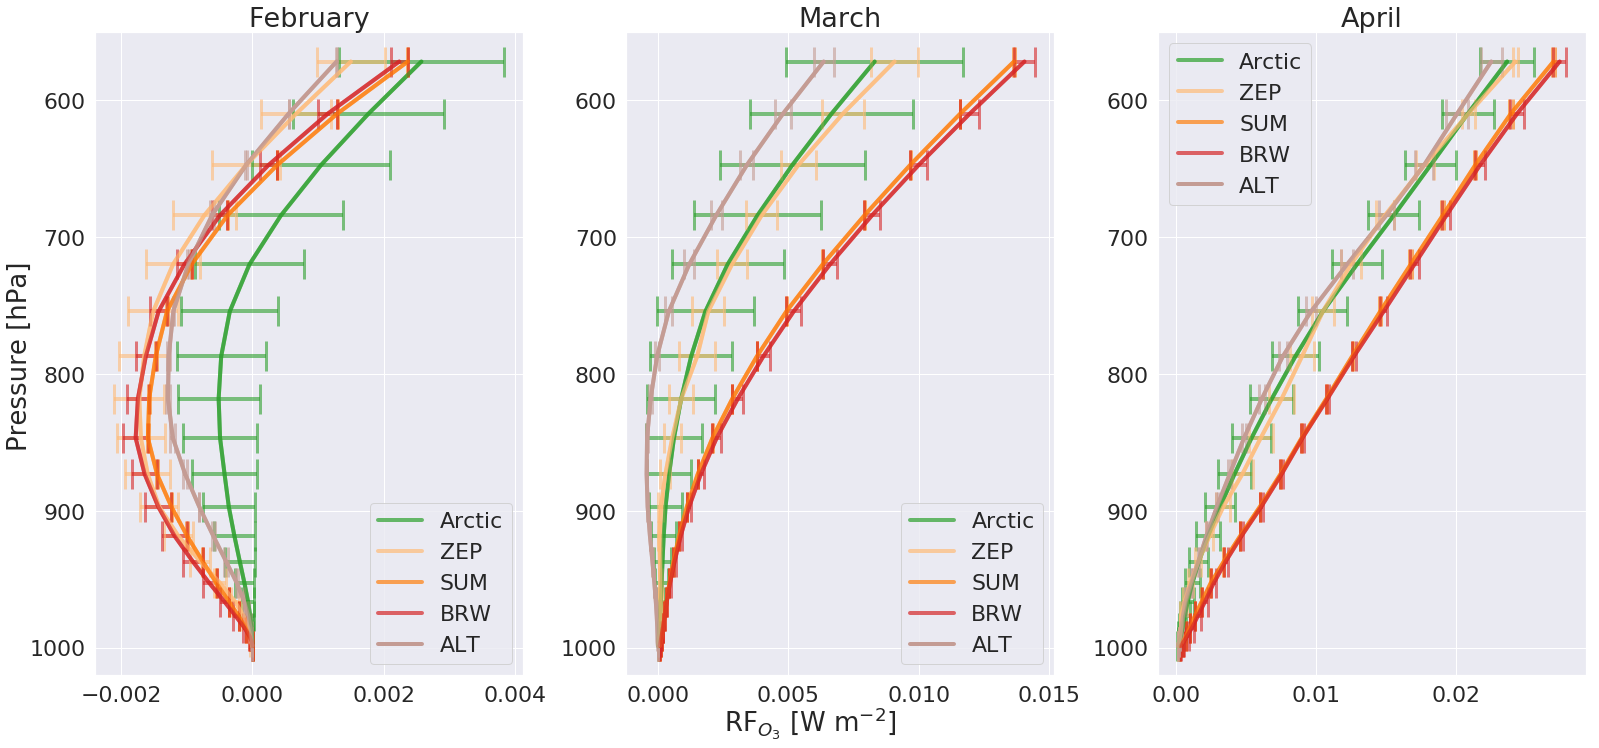
\includegraphics[width = \linewidth]{Chapter6_Results/images/RF/vert_RF_FebApr_2001.png}
    \caption{Monthly mean averaged RF (in Wm$^{-2}$) in each model layer (layer 1-60) averaged over the whole Arctic (defined as above 68$^o$N) (green line), over Zeppelin (77.0-80.5$^o$N, 10.5-13.5$^o$E) (yellow line), over Summit (71.0-74.0$^o$N, 40.0-37.0$^o$W)(orange line), over Barrow (70.0-73.0$^o$N, 40.0-37.0$^o$W)(red line) and over Alert (80.5-84.5$^o$N, 64.0-61.0$^o$W)(purple line). Errorbars indicate the standard deviation in the layer. The profiles are shown for the months February (left), March (middle) and April (right) in 2001}
    \label{fig:vert_RF_FebApr_2001}
\end{figure}
\begin{figure}[ht]
    \centering
    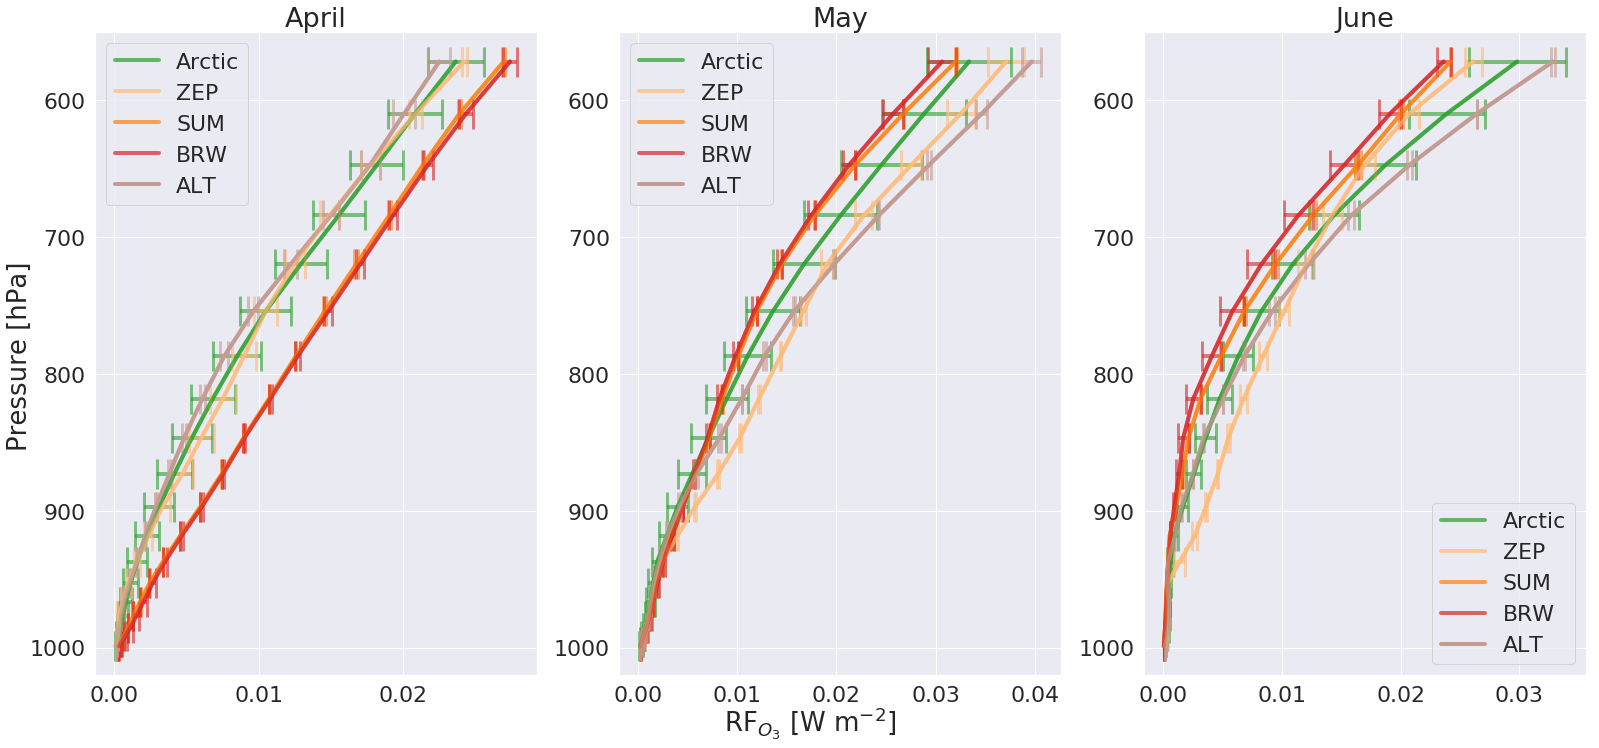
\includegraphics{Chapter6_Results/images/RF/vert_RF_AprJune_2001.png}
    \caption{Monthly mean averaged RF (in Wm$^{-2}$) in each model layer (layer 1-60) averaged over the whole Arctic (defined as above 68$^o$N) (green line), over Zeppelin (77.0-80.5$^o$N, 10.5-13.5$^o$E) (yellow line), over Summit (71.0-74.0$^o$N, 40.0-37.0$^o$W)(orange line), over Barrow (70.0-73.0$^o$N, 40.0-37.0$^o$W)(red line) and over Alert (80.5-84.5$^o$N, 64.0-61.0$^o$W)(purple line). Errorbars indicate the standard deviation in the layer. The profiles are shown for the months April (left), May (middle) and June (right) in 2001}
    \label{fig:vert_RF_AprJune_2001}
\end{figure}


% diff_mean_SUM = find_stats_lev(diff, 'mean', 'O3_RF', 71.0, 74.0, 180-40.0, 180-37.0)
% diff_std_SUM = find_stats_lev(diff, 'std', 'O3_RF', 71.0, 74.0, 180-40.0, 180-37.0)
% diff_mean_ALT = find_stats_lev(diff, 'mean', 'O3_RF', 80.5, 84.5, 180-64.0, 180-61.0)
% diff_std_ALT = find_stats_lev(diff, 'std', 'O3_RF', 80.5, 84.5, 180-64.0, 180-61.0)
% diff_mean_BRW = find_stats_lev(diff, 'mean', 'O3_RF', 70.0, 73.0, 180-40.0, 180-37.0)
% diff_std_BRW = find_stats_lev(diff, 'std', 'O3_RF', 70.0, 73.0, 180-40.0, 180-37.0)
% diff_mean_ZEP = find_stats_lev(diff, 'mean', 'O3_RF', 77.0, 80.5, 180+10.5, 180+13.5)
% diff_std_ZEP = find_stats_lev(diff, 'std', 'O3_RF', 77.0, 80.5, 180+10.5, 180+13.5)